\RequirePackage{silence} % :-\
    \WarningFilter{scrbook}{Usage of package `titlesec'}
    \WarningFilter{titlesec}{Non standard sectioning command detected}
\documentclass[11pt,paper=b5,footinclude,headinclude]{scrbook} % KOMA-Script book
\usepackage[T1]{fontenc}
\usepackage[style=arsclassica, parts=false, eulermath=false, palatino=true, eulerchapternumbers=true]{classicthesis}

\usepackage{afterpage}
\usepackage{xcolor}
\usepackage{xspace}
\usepackage{etoolbox}
\providetoggle{long}


%framed example
\usepackage[framemethod=TikZ]{mdframed}
% EXAMPLES
%% set the counter for your environment
\newcounter{example}
\renewcommand{\theexample}{\thechapter.\arabic{example}}

%% define the style
\mdfdefinestyle{example}{%
    linecolor=blue,
    backgroundcolor=blue!5,
    outerlinewidth=2pt,
    bottomline=false,
    leftline=false,rightline=false,
    skipabove=\baselineskip,
    skipbelow=\baselineskip,
    frametitle=\mbox{},
}
%% setup the environments
%%% with number
\newmdenv[%
    style=example,
    settings={\global\refstepcounter{example}},
    frametitlefont={\bfseries Zgled~\theexample\quad},
]{example}
%%% without number (starred version)
\newmdenv[%
    style=example,
    frametitlefont={\bfseries Zgled~\quad},
]{example*}



\newcommand{\komentar}[1]{\textcolor{red}{[#1]}} %for displaying red texts

\usepackage{fullpage}
%\usepackage{fancyhdr}
\usepackage{enumerate}


\usepackage[slovene]{babel} % slovenske nastavitve (naslovi, deljenje besed ...)
\usepackage[utf8]{inputenc}
\usepackage{amsfonts,amssymb}
\usepackage{graphicx}
\usepackage{amsmath,amssymb,amsthm}
\usepackage{epsf}
\usepackage{epsfig}
\usepackage{graphics}
\usepackage{color}
\usepackage{comment}
%\usepackage{times}
%\usepackage{txfonts}
\def\P {{\cal P}}
\def\ali {{~\vee~}}
\def\inn {{~\wedge~}}
\def\sledi {{~\Rightarrow~}}
\def\brez {{\,\setminus\,}}
\def\cee {{~\Leftrightarrow~}}
\def\zgled{\noindent\textbf{\color{blue} Zgled: }}
\def\kz{{\hfill{\color{blue}$\blacktriangle$}}}% konec zgleda
%\parskip=7pt
%
%\textwidth=17cm\textheight=22cm\parindent=15pt\parskip=5pt
%\oddsidemargin=-5mm  \headheight=0pt \pagestyle{plain}

%spremenljivke
\newcommand{\myTitle}{Teoretične osnove računalništva\xspace}
\newcommand{\mySubtitle}{Diskretne strukture za računalničarje \xspace} 				%dodaj podnaslov if needed
\newcommand{\myName}{UP FAMNIT \xspace}
\newcommand{\myPublisher}{XXX}
\newcommand{\myMonth}{Pomlad}
\newcommand{\myYear}{2021}
\newcommand{\verzija}{Verzija 0.1 }
\newcommand{\shortAuthors}{M. Krnc, Š. Miklavič, M. Milanič, R. Požar, P. Škraba}
\newcommand{\myAuthors}{Matjaž Krnc, Štefko Miklavič, \\Martin Milanič, Rok Požar, Primož Škraba}
\newcommand{\frontpageAuthors}{Matjaž Krnc, Štefko Miklavič,\\[3mm] Martin Milanič, Rok Požar, Primož Škraba}

\newcommand{\myISBN}{978-961-XXX-XXX-X }


\newtheorem*{trditev}{Trditev}
\newtheorem*{izrek}{Izrek}
\newtheorem*{problem}{Naloga}
\newtheorem*{lema}{Lema}
\newtheorem*{posledica}{Posledica}
\newtheorem*{definicija}{Definicija}
\newtheorem*{zg}{Zgled}


\begin{document}
%*******************************************************
% Titlepage
%*******************************************************
\begin{titlepage}
\definecolor{amber}{rgb}{1.0, 0.75, 0.0}
\pagecolor{amber}\afterpage{\nopagecolor}
	% if you want the titlepage to be centered, uncomment and fine-tune the line below (KOMA classes environment)
	\begin{addmargin}[-1cm]{-1cm}
    \begin{center}
        \large  

        \hfill

        \vfill

        \begingroup
            \color{Maroon}\spacedallcaps{\LARGE\myTitle} \\ \bigskip
        \endgroup

        \spacedlowsmallcaps{\mySubtitle}

        \vfill

        \includegraphics[width=10cm]{Desargues.png} %\\ \medskip
				\vfill
        \textsc{\Large\frontpageAuthors}   
        \vfill   

        \myMonth \xspace \myYear \ -- \verzija

        \vfill                      

    \end{center}  
  \end{addmargin}       
\end{titlepage}   

%\begin{addmargin}[-1cm]{-1cm}
	{\vspace*{\fill}
	\setlength{\fboxsep}{6mm}
	\noindent\fbox{
	\begin{minipage}[b][6.5cm][c]{11cm} % velikost okvira škatle je 11 cm
							% x 6,5 cm
	\small
	CIP -- Katalo\v zni zapis o publikaciji\\
	Narodna in univerzitetna knji\v znica, Ljubljana
	
	\vfill

	123.4(567)(8.901.2)
	\vfill

	TEORETIČNE osnove računalništva [Elektronski vir] : Diskretne strukture za računalničarje / avtorji \shortAuthors; [urednik] M. Krnc. - Verzija \myVersion.  - El. knjiga. - Ljubljana : samozal. M. Krnc, 2020.
	\vfill
	
	Način dostopa (URL):\\ \url{https://github.com/mkrnc/TOR1-zapiski-s-predavanj}
	
	\vfill
	
	ISBN \myISBN  (pdf)\\
	%1. Milanič, Martin 2. Krnc, Matjaž, 1987-
	123456789
	\vfill
	
	\end{minipage}}}
%\end{addmargin}
\endinput
\newpage
\section*{Predgovor}
Pred tabo so zapiski iz predavanj za predmet TOR1, ki se predava študentom prvega letnika na FAMNIT, Univerza na Primorskem.
Predmet pokriva osnove iz različnih področij teoretičnega računalništva in je usmerjen potrebam računalničarjev.
%Od leta 2020 naprej sem se odločil tale TeX projekt odpreti kot javni repozitorij, tako da lahko zares vsak študent predlaga svoje naloge (oz. rešitve), ki se jih ustrezno vključi v tole skripto.

Gradivo je osnovano na izročkih  predhodnih predavateljev istega predmeta, ter na knjigi: 
\begin{quote}
   Niko Prijatelj (1996):
   \emph{Matematične strukture 1}.
   \\
   Društvo   matematikov,   fizikov in astronomov Slovenije. 
\end{quote}

Dokument je zamišljen kot dopolnjevanje predavanj, in se ga ne sme jemati kot samostojno gradivo za pripravo na izpit. 
Morebitna vprašanja in najdene napake, lepo prosim, sporočite na
\url{matjaz.krnc@upr.si}, oz. ustvarite t.i. "issue"\xspace na našem javnem repozitoriju.
\begin{center}
    \url{https://github.com/mkrnc/TCS1-course-notes.git}.    
\end{center}

\medskip
Gradivo je osnovano na nekaterih starejših izročkih od mojih predhodnih predavateljev tega istega predmeta, med katerimi so 
\begin{center}
    prof. \textbf{M. Milanič}, 
    prof. \textbf{N. Prijatelj}, ter 
    prof. \textbf{P. Škraba}.
\end{center}

%Among most notable student contributors are:

\newpage
\vspace*{\fill}
\noindent

\begin{tabular}{ll}
%Lektorirala: ...\\[3mm]
\multicolumn{2}{ l }{\textbf{\myTitle}} \\
\multicolumn{2}{ l }{\emph{\mySubtitle}} \\[6mm]
\textbf{Urednik:} & Matjaž Krnc\\[3mm]
\textbf{Avtorji:} & \parbox[t]{6cm}{\myAuthors \vspace{3mm}}\\
\textbf{Samozaložba in oblikovanje:} & Matjaž Krnc\\[3mm]
%E-po�ta: knjiga@vidra.net\\[3mm]
%Za zalo�bo: Andrej Klemenc\\[3mm]
%\textbf{Oblikovanje:} & Matjaž Krnc\\[3mm]
\textbf{ISBN:} &  \myISBN \\
%Priprava za tisk: \\[3mm]
%Tisk: \\[3mm]
Ljubljana, \myMonth\xspace\myYear
\end{tabular}
\endinput

\tableofcontents


\chapter{Matematična logika}

Kaj je izjava? {\em Trdilna izjava}, ki je bodisi pravilna ali pa nepravilna.\footnote{Izjave boste podrobneje obravnavali na uvodnem predavanju pri Analizi I.}

\medskip
Prispevek logike k znanju je v odkrivanju novih izjav, ki so logične posledice drugih.
\begin{itemize}
  \item Celotno teorijo naravnih števil je moč zgraditi iz 5 osnovnih izjav,
  ki jih običajno imenujemo Peanovi aksiomi. Teh pet izjav lahko z besedico ``in"~povežemo v eno samo
  izjavo.
  \item Hilbert je pokazal, da je vso kopico izrekov elementarne geometrije moč dokazati iz 20 aksiomov
  (osnovnih izjav).
  \item V splošnem so matematične strukture definirane s peščico aksiomov,
  iz katerih se s pomočjo logičnega sklepanja izpelje izreke in gradi teorije.
\end{itemize}

O razvoju logike in teorije množic si lahko preberete v Prijateljevi knjigi (Osnove matematične logike, 1.~poglavje, 2.~podpoglavje).

\section{Vezniki med logičnimi izjavami}

\textbf{ \underline{Negacija:}} Ne $A$; ni res, da $A$

Oznaka: $\neg A$.

$\neg A$ je negacija izjave $A$. Izjava $\neg A$ je pravilna, če je $A$ nepravilna, in je nepravilna,
če je $A$ pravilna.

Zgled: {\em Jutri bo dež. Negacija: Jutri ne bo dežja. (Ni res, da bo jutri dež.)}

\medskip
Vrednost vsake sestavljene izjave je enolično določena z vrednostmi osnovnih izjav, ki v njej nastopajo.
Za nazoren pregled te odvisnosti si pomagamo s t.i.~{\em pravilnostnimi tabelami}.
Dogovorimo se, da bomo vrednost {\em pravilno} označevali z~1, vrednost {\em nepravilno} pa z~0.

Pravilnostna tabela za negacijo:
$$\begin{tabular}{c|c|c}
  \hline
  % after \\: \hline or \cline{col1-col2} \cline{col3-col4} ...
   & $A$ & $\neg A$ \\
  \hline
  1. & 1 & 0 \\
  2. & 0 & 1 \\
\end{tabular}$$

\medskip
\textbf{ \underline{Konjunkcija:}} $A$ in $B$

Oznaka: $A\inn  B$

$A\wedge B$ je konjunkcija izjav $A$ in $B$. Ta sestavljena izjava je pravilna,
kadar sta obe izjavi $A$ in $B$ pravilni, in nepravilna sicer.

Zgled: {\em Sneg pada. Veter piha. Konjunkcija: Sneg pada in veter piha.}

\medskip
\textbf{ \underline{Disjunkcija:}} $A$ ali $B$ (inkluzivno)

Oznaka: $A\ali B$

$A\ali B$ je disjunkcija izjav $A$ in $B$. Ta sestavljena izjava je pravilna,
brž ko je ena izmed izjav  $A$ in $B$ pravilna, in nepravilna sicer.

Zgled: {\em Janez bo jutri vprašan fiziko. Janez bo jutri vprašan matematiko.
Disjunkcija: Janez bo jutri vprašan fiziko ali matematiko.}

\medskip
\textbf{ \underline{Implikacija:}} Če $A$, potem $B$

Oznaka: $A\sledi B$

$A\sledi B$ je implikacija izjav $A$ in $B$. Ta sestavljena izjava je nepravilna,
kadar je $A$ pravilna, $B$ pa nepravilna. V vseh ostalih primerih je pravilna.

$A$ - antecedens, zadostni pogoj

$B$ - konsekvens

\begin{example*}
Če Andrej naredi maturo, potem mu kupim kolo.
\end{example*}


\medskip
\textbf{ \underline{Ekvivalenca:}} $A$ če in samo če $B$

Oznaka: $A\cee B$

$A\cee B$ je ekvivalenca izjav $A$ in $B$. Ta sestavljena izjava je pravilna,
kadar sta izjavi $A$ in $B$ ali obe pravilni ali obe nepravilni.
V vseh ostalih primerih je nepravilna.

"$A\cee B$" beremo:

$A$ če in samo če $B$

$A$ tedaj in samo tedaj kot $B$

$A$ natanko tedaj kot $B$

\begin{example*} {\em Andreju kupim kolo, če in samo če naredi maturo.}
\end{example*}

\medskip
\textbf{ Pravilnostne tabele za konjuncijo, disjunkcijo, implikacijo in ekvivalenco:}
$$\begin{tabular}{c|c|c|c|c|c}
  \hline
  % after \\: \hline or \cline{col1-col2} \cline{col3-col4} ...
   & $A, B$ & $A \inn B$ & $A \ali B$ & $A \sledi B$ & $A \cee B$ \\
  \hline
  1. & 1, 1 & 1 & 1 & 1 & 1 \\
  2. & 1, 0 & 0 & 1 & 0 & 0  \\
  3. & 0, 1 & 0 & 1 & 1 & 0  \\
  4. & 0, 0 & 0 & 0 & 1 & 1 \\
\end{tabular}$$

\medskip

Izjave, dobljene z uprabo $5$ osnovnih povezav, so \emph{ sestavljene}. V splošnem pravimo, da je dana izjava \emph{ sestavljena}, če je izid
zaporedne uporabe $5$ osnovnih povezav na osnovnih izjavah $A_1,\ldots, A_n$, pa tudi na izjavah, ki smo jih že prej napravili.
Dvomom o tem, katera povezava sledi prej in katera pozneje, se izognemo z uporabo oklepajev.
Uporabo oklepajev pa z uporabo naslednjega dogovora omejimo, kolikor se da:
\begin{itemize}
  \item Kadar izjava nastopa osamljeno, je ne oklenemo z oklepaji:

  npr.: namesto $(A\inn B)$ pišemo $A\inn B$

  \item Kadar ista vrsta povezave nastopi večkrat zapored, jo obravnavamo z leve proti desni.

  npr.: namesto $((A\inn B) \inn C) \inn D$ pišemo $A\inn B \inn C\inn D$

  \item Upoštevamo naslednji prednostni red operacij:
  $\neg$, $\ali$, $\inn$, $\sledi$, $\cee$ (v vsaki sestavljeni izjavi najprej upoštevamo negacije, za njimi disjunkcije itd.)

  npr.: namesto $(A\inn B) \sledi (\neg C)$ pišemo  $A\inn B \sledi\neg C$
\end{itemize}

\medskip
Pravilnostne tabele lahko zapišemo tudi za sestavljene izjave, z uporabo poljubnega
zaporedja, s katerim sestavimo izjavo.

\begin{example*}
Zapišimo  izjavo
\begin{equation}\label{eq:izjava2}
\mathcal I\sim(A \sledi B) \inn (B\sledi C) \inn  (\neg A \ali C)
\end{equation}
ter označimo  
\[
\mathcal I' \sim (A \sledi B) \inn (B\sledi C)
\]

$$\begin{tabular}{c|c|c|c|c|c|c|c}
  \hline
  % after \\: \hline or \cline{col1-col2} \cline{col3-col4} ...
   & $A, B, C$ & $A \sledi B$ & $B \sledi C$ & $\mathcal I'$ & $\neg A$ & $\neg A \ali C$ & $\mathcal I$\\
  \hline
  1. & 1, 1, 1 & 1 & 1 & 1 & 0 & 1 & 1 \\
  2. & 1, 1, 0 & 1 & 0 & 0 & 0 & 0 & 0 \\
  3. & 1, 0, 1 & 0 & 1 & 0 & 0 & 1 & 0 \\
  4. & 1, 0, 0 & 0 & 1 & 0 & 0 & 0 & 0 \\
  5. & 0, 1, 1 & 1 & 1 & 1 & 1  & 1 & 1 \\
  6. & 0, 1, 0 & 1 & 0 & 0 & 1  & 1 & 0 \\
  7. & 0, 0, 1 & 1 & 1 & 1 & 1  & 1 & 1 \\
  8. & 0, 0, 0 & 1 & 1 & 1 & 1  & 1 & 1 \\
\end{tabular}$$

\end{example*}

\bigskip
Naj bo $A$ izjava, sestavljena iz osnovnih izjav $A_1,\ldots, A_n$.

{\em Določilo izjave $A$}: določitev vrednosti 1 / 0 (pravilno / nepravilno) vsaki od izjav $A_1,\ldots, A_n$

\iftoggle{long}{\noindent\komentar{Izpuščeno: OD TU}\\}
{
{\color{blue}
{\em Prostor izjave}: vsa različna mogoča določila, ki pripadajo tej izjavi.
}\\
}

Če je izjava sestavljena iz $n$ osnovnih izjav, potem ima izjava natanko $2^n$ določil.

{
{\color{blue}
{\em Podprostor pravilnosti}: določila, pri katerih je izjava pravilna.}\\
}

\iftoggle{long}{\komentar{Izpuščeno: DO TU}\\}

Dve vrsti izjav si zaslužita posebno ime:
\begin{itemize}
  \item {\em Tavtologija}: pri vseh določilih pravilna izjava (primer: $A\ali \neg A$)
%  , podprostor pravilnosti je enak celotnemu prostoru izjave
  \item {\em Protislovje}: pri vseh določilih nepravilna izjava (primer: $A\inn \neg A$)
  %, podprostor pravilnosti je prazen
\end{itemize}

\begin{example*}
Za vsako od naslednjih dveh izjav s pomočjo pravilnostne tabele določi, ali je izjava tavtologija in ali je protislovje.
\begin{enumerate}[(a)]
  \item $(A\sledi B) \sledi A\ali B$,
  \item $(A\sledi B) \cee A\inn \neg B$.
\end{enumerate}

Pravilnostna tabela za prvo izjavo:
$$\begin{tabular}{c|c|c|c|c}
  \hline
  % after \\: \hline or \cline{col1-col2} \cline{col3-col4} ...
   & $A, B$ & $A\sledi B$ & $A \ali B$ & $(A\sledi B) \sledi A\ali B$\\
  \hline
  1. & 1, 1 & 1 & 1 & 1 \\
  2. & 1, 0 & 0 & 1 & 1  \\
  3. & 0, 1 & 1 & 1 & 1   \\
  4. & 0, 0 & 1 & 0 & 0  \\
\end{tabular}$$
Izjava ni ne tavtologija ne protislovje.

\medskip
Pravilnostna tabela za drugo izjavo:
$$\begin{tabular}{c|c|c|c|c|c}
  \hline
  % after \\: \hline or \cline{col1-col2} \cline{col3-col4} ...
   & $A, B$ & $A\sledi B$ & $\neg B$ & $A\inn \neg B$ & $(A\sledi B) \cee A\inn \neg B$\\
  \hline
  1. & 1, 1 & 1 & 0 & 0 & 0 \\
  2. & 1, 0 & 0 & 1 & 1 & 0 \\
  3. & 0, 1 & 1 & 0 & 0 & 0 \\
  4. & 0, 0 & 1 & 1 & 0 & 0 \\
\end{tabular}$$
Izjava ni tavtologija, je pa protislovje.
\end{example*}

\bigskip

\textbf{ Domača naloga:}

%\textbf{ 1.} Preštudiraj dodatno gradivo o izjavah, objavljeno na e-učilnici.

\medskip
\textbf{ 1.}  Dani sta izjavi $A$: ``Andrej govori francosko.'' in $B$: ``Andrej govori dansko.''
V naravnem jeziku zapiši naslednje sestavljene izjave:

(a) $A\ali B$

(b) $A\inn B$

(c) $A\inn \neg B$

(d) $\neg A\ali \neg B$

(e) $\neg \neg A$

(f) $\neg (\neg A\inn \neg B)$

\medskip
\textbf{ 2.}  Dani sta izjavi $A$: ``Janez je bogat.'' in $B$: ``Janez je srečen.''

Naslednje izjave zapiši simbolično:

(a) Če je Janez bogat, potem je nesrečen.

(b) Janez ni niti srečen niti bogat.

(c) Janez je srečen, samo če je reven.

(d) Janez je reven natanko tedaj, ko je nesrečen.


\subsection*{Vitezi in oprode}

S pomočjo pravilnostnih tabele lahko rešujemo uganke o vitezih in oprodah.
Vitezi vselej govorijo resnico, oprode pa vselej lažejo.

\textbf{ Naloga:} Artur in Bine podata naslednji izjavi:
\begin{itemize}
  \item Artur: ``Bine je oproda."
  \item Bine: ``Nobeden od naju ni oproda."
\end{itemize}
Za vsakega od njiju določi, ali je vitez ali oproda!

\medskip
Naj bo $A$ izjava: ``Artur je vitez,"~$B$ pa izjava: ``Bine je vitez."

\medskip
Določimo pravilnost izjav $A$ in $B$ s pomočjo pravilnostne tabele.
Iz Arturjeve izjave~sklepamo na pravilnost izjave
$A\cee \neg B$. Iz Binetove izjave~sklepamo na pravilnost izjave
$B\cee A\inn B$. Torej je konjunkcija teh dveh izjav pravilna:
$$(A\cee \neg B)\inn (B\cee A\inn B)\,.$$
Za kateri nabor določil za $A$ in $B$ je ta izjava pravilna?
$$\begin{tabular}{c|c|c|c|c|c|c}
  \hline
  % after \\: \hline or \cline{col1-col2} \cline{col3-col4} ...
   $A$ &  $B$ & $\neg B$ & $A \cee \neg B$ & $A \inn B$ & $B\cee A\inn B$ & $(A\cee \neg B)\inn (B\cee A\inn B)$ \\
  \hline
1 & 1 & 0 & 0 & 1 & 1 & 0\\
1& 0 & 1 & 1 & 0 & 1 & 1\\
0& 1 & 0 & 1 & 0 & 0 & 0\\
0& 0 & 1 & 0 & 0 & 1 & 0\\
\end{tabular}$$
Artur je vitez, Bine pa oproda.\qed

\bigskip
\textbf{ Še ena podobna naloga:} Tokrat podata Artur in Bine naslednji izjavi:
\begin{itemize}
  \item Artur: ``Jaz in Bine nisva iste vrste."~
  \item Bine: ``Natanko eden od naju je vitez."
\end{itemize}

\medskip
Naslednja konjunkcija izjav je pravilna:
\begin{equation}\label{eq:izjava3}
[A\cee (A\inn \neg B) \ali (\neg A \inn B)]\inn [B\cee (A\inn \neg B) \ali (\neg A \inn B)]\,.
\end{equation}
$$\begin{tabular}{c|c|c|c|c|c|c|c}
  \hline
  % after \\: \hline or \cline{col1-col2} \cline{col3-col4} ...
   $A$ &  $B$ & $A\inn \neg B$ & $\neg A\inn B$ & $(A\inn \neg B) \ali (\neg A \inn B)~(*)$ & $B\cee (*)$ & $A\cee (*)$ & (\ref{eq:izjava3})\\
  \hline
1& 1 & 0 & 0 & 0 & 0 & 0 & 0\\
1& 0 & 1 & 0 & 1 & 1 & 0 & 0\\
0& 1 & 0 & 1 & 1 & 0 & 1 & 0\\
0& 0 & 0 & 0 & 0 & 1 & 1 & 1\\
\end{tabular}$$
Oba sta oprodi.\qed

\medskip

\textbf{ Domača naloga:} Reši naslednji nalogi o vitezih in oprodah:
\begin{itemize}
  \item Artur: ``Ni res, da je Bine oproda."~Bine: ``Nisva oba iste vrste."
  \item Artur: ``Ni res, da je Cene oproda."~Bine: ``Cene je vitez ali pa sem jaz vitez."~Cene: ``Bine je oproda."
\end{itemize}
\qed


Videli smo, kako priredimo vsaki sestavljeni izjavi njeno pravilnostno tabelo.
Obratna naloga: Če imamo dane neodvisne izjave $A_1,\ldots, A_n$,
kako konstruirati iz njih sestavljeno izjavo, ki bo imela
pri vsakem izmed $2^n$ določil {\em vnaprej predpisano logično vrednost?}

Da bi rešili to nalogo, si najprej poglejmo t.i.~{\em logične ekvivalence}.

\section{Logične ekvivalence}

Naj bosta $B$ in $C$ izjavi, sestavljeni iz izjav $A_1,\ldots, A_n$.
\iftoggle{long}{
{\color{blue}
Če je izjava $B\cee C$ tavtologija, pravimo, da sta $B$ in $C$ {\em logično ekvivalentni}.
}
}
{
Če je izjava $B\cee C$ tavtologija, pravimo, da sta $B$ in $C$ {\em logično ekvivalentni}.
}
Za logiko: $B = C$ (dve  različni obliki iste izjave).

Naštejmo najpoglavitnejše logične ekvivalence:
\begin{enumerate}
  \item $A \cee \neg(\neg A)$, zakon dvakratne negacije
  \item $A\inn B\cee B \inn A$,~~~$A\ali B\cee B \ali A$, komutativnost konjunkcije in disjunkcije
  \item $A\inn (B\inn C) \cee (A\inn B)\inn C$,~~~$A\ali (B\ali C) \cee (A\ali B)\ali C$, asociativnostna zakona
   \item $A\ali (B\inn C) \cee (A\ali B) \inn (A\ali C)$, ~~~~
   $A\inn (B\ali C) \cee (A\inn B) \ali (A\inn C)$, distributivnostna zakona
   \item $A\inn A\cee A$, ~~~~$A\ali A \cee A$
   \item $\neg(A\inn B)\cee \neg A \ali \neg B$
   \item $\neg(A\ali B)\cee \neg A \inn \neg B$, De Morganova zakona (6. in 7.)
   \item $(A\sledi B) \cee (\neg B\sledi \neg A)$
   \item $(A\sledi B) \cee \neg A\ali B$
   \item $(A\sledi B) \cee \neg(A\inn \neg B)$
   \item $(A\cee B) \cee (A\sledi B) \inn (B\sledi A)$
  \item $(A \cee B) \cee (B\cee A)$,  komutativnost ekvivalence
  \item $(A \cee B) \cee (\neg A\cee \neg B)$
  \item $(A \cee B) \cee (\neg A\ali B)\inn (A\ali \neg B)$
  \item $(A \cee B) \cee (A\inn B)\ali (\neg A\inn \neg B)$
  \item $\neg(A \cee B) \cee (A\cee \neg B)$
\end{enumerate}

Za vajo se prepričajmo v pravilnost 16.~ekvivalence s pomočjo pravilnostne tabele:
$$\begin{tabular}{c|c|c|c|c|c}
  \hline
  % after \\: \hline or \cline{col1-col2} \cline{col3-col4} ...
   & $A, B$ & $A \cee B$ & $\neg(A \cee B)$ & $\neg B$ & $A \cee \neg B$ \\
  \hline
  1. & 1, 1 & 1 & 0 & 0 & 0 \\
  2. & 1, 0 & 0 & 1 & 1 & 1  \\
  3. & 0, 1 & 0 & 1 & 0 & 1  \\
  4. & 0, 0 & 1 & 0 & 1 & 0 \\
\end{tabular}$$

\textbf{ Domača naloga:} S pomočjo pravilnostnih tabel (ali kako drugače) se prepričaj v pravilnost
preostalih ekvivalenc.

\bigskip
S pomočjo zgornjih ekvivalenc se lahko prepričamo, da $5$ osnovnih povezav med izjavami ni med seboj neodvisnih.
Vse sestavljene izjave lahko izrazimo {\em samo z dvema osnovnima povezavama}, če ju le primerno izberemo.
Zadošča že:
\begin{enumerate}
  \item[\textbf{ (a)}] negacija $\neg$ in  disjunkcija $\ali$
  \item[\textbf{ (b)}] negacija $\neg$ in konjunkcija $\inn$
  \item[\textbf{ (c)}] negacija $\neg$ in implikacija $\sledi$
\end{enumerate}
Te izbire so edine mogoče.

\medskip
\begin{example*}

Vzemimo izjavo ``Če je kakšna reč lepa, potem je minljiva."

($\neg$ in $\ali$) Reč ni lepa, ali pa je minljiva.

($\neg$ in $\inn$) Ni res, da je kakšna reč lepa in ni minljiva.

($\neg$ in $\sledi$) Če kakšna reč ni minljiva, potem ni lepa.\end{example*}

% 2. predavanje (2018) - konec

\section{Izbrani obliki izjav}

Od zadnjič dolgujemo še rešitev naslednje naloge: iz danih izjav $A_1,\ldots, A_n$ konstruiraj izjavo,
ki bo imela pri vsakem izmed $2^n$ določil vnaprej predpisano vrednost.

\textbf{ 1. način:}
Vsakemu določilu $d$ za izjave $A_1,\ldots, A_n$ priredimo konjunkcijo
$$C_1\inn \ldots \inn C_n\,,$$
in sicer takole: izjava je $C_i = A_i$, če ima $A_i$ v določilu $d$ vrednost 1, in naj bo
$C_i = \neg A_i$, sicer.
Tako dobljena konjunkcija je pravilna pri določilu $d$ in nepravilna pri vsakem drugem določilu.
Imenuje se {\em osnovna konjunkcija določila $d$}.

Sedaj pa napravimo osnovne konjunkcije natanko tistih določil, za katere naj
bo iskana izjava pravilna, in jih povežimo z disjunkcijami!

Tako dobljeno izjavo imenujemo {\em izbrana disjunktivna oblika.}

Ta postopek deluje v vsakem primeru, le v primeru protislovja ne! Za protislovje lahko iskano izjavo
konstruiramo posebej, npr.~$A_1\inn \neg A_1$.

\bigskip
\textbf{ 2. način:}

$d$ - določilo

Sedaj tvorimo {\em osnovno disjunkcijo določila $d$}:
$$D_1\ali \cdots \ali D_n\,,$$
kjer je

$D_i = \neg A_i$, če ima $A_i$ v $d$ vrednost 1 in

$D_i = A_i$, če ima $A_i$ v $d$ vrednost 0.

Tako dobljena disjunkcija je nepravilna pri $d$  in pravilna pri vsakem drugem določilu.

Napravimo osnovne disjunkcije natanko tistih določil, za katere naj bo iskana sestavljena izjava nepravilna,
in jih povežimo med seboj s konjunkcijami.

Tako dobljeno izjavo imenujemo {\em izbrana konjunktivna oblika.}

Ta postopek deluje v vsakem primeru, le v primeru tavtologije ne! Za tavtologijo
lahko konstruiramo iskano izjavo posebej, npr.~$A_1\ali \neg A_1$ (``zakon izključene tretje možnosti", vsaka
izjava je bodisi pravilna bodisi nepravilna).

\bigskip
\textbf{ Zgled:}
Iščemo izjavo $D$, sestavljeno iz izjav $A, B$ in $C$, za katero velja:
$$\begin{tabular}{c|c|c|c|c|c}
  \hline
  % after \\: \hline or \cline{col1-col2} \cline{col3-col4} ...
$A$ & $B$ & $C$  & $D$ & osnovna konjunkcija & osnovna disjunkcija \\
  \hline
1 & 1 & 1 & 1 & $A \inn B \inn C$ & \\
1 & 1 & 0 & 0 & & $\neg A\ali\neg B \ali C$ \\
1 & 0 & 1 & 0 &  & $\neg A\ali B \ali \neg C$ \\
1 & 0 & 0 & 0 &  & $\neg A\ali B \ali C$ \\
0 & 1 & 1 & 1 & $\neg A \inn B\inn C$& \\
0 & 1 & 0 & 0 & & $A\ali\neg B \ali C$ \\
0 & 0 & 1 & 1 & $\neg A\inn \neg B\inn C$ &  \\
0 & 0 & 0 & 1 & $\neg A\inn \neg B\inn \neg C$ &  \\
\end{tabular}$$
Izbrana disjunktivna oblika izjave $D$ je
$$(A\inn B\inn C) \ali (\neg A\inn B\inn C)\ali (\neg A\inn \neg B\inn C)\ali (\neg A\inn \neg B\inn \neg C)\,.$$
izbrana konjunktivna oblika pa je
$$(\neg A\ali\neg B \ali C) \inn (\neg A\ali B \ali \neg C)\inn
(\neg A\ali B \ali C) \inn (A\ali \neg B \ali C)\,.$$\qed



{
\begin{example*}

Recimo, da so vas ujeli ljudožerci v Afriki. Njihov poglavar pa se odlikuje z izrednim smislom za humor
in z ljubeznijo do logike. Zato vas spravi v ječo z dvema izhodoma
in veli takole: ``En izhod iz ječe vodi neposredno v kotel, drugi pa v zlato svobodo. Premisli in izberi!
Da ti bo izbira lažja, ti dajem v pomoč dva svoja hrabra vojščaka in enemu od njih smeš
postaviti eno samo vprašanje. Vendar pomni! Eden od njiju govori vedno resnico, medtem ko drugi
neprestano laže."

Zadeva ni rožnata, vendar se s pomočje logike lahko izognete kotlu.
Kakšno vprašanje boste postavili?

Naj bo $A$ izjava ``Prvi izhod vodi v svobodo."  in $B$ izjava ``Vi govorite resnico."
Iz teh dveh izjav je treba sestaviti tako izjavo, da bo odgovor ``da"~nanjo pomenil, da je
izjava $A$ pravilna in odgovor ``ne"~pa, da je izjava $A$ nepravilna, in sicer ne glede na to,
katerega od obeh vojščakov boste vprašali. Označimo iskano izjavo s $C$. Potem mora veljati:

$$\begin{tabular}{c|c|c|c|c}
  \hline
  % after \\: \hline or \cline{col1-col2} \cline{col3-col4} ...
$A$ & $B$ & $C$  & osnovna konjunkcija & osnovna disjunkcija \\
  \hline
1 & 1 & 1 & $A\inn B$ & \\
1 & 0 & 0 & & $\neg A\ali B$ \\
0 & 1 & 0 &  & $A\ali\neg B$   \\
0 & 0 & 1 & $\neg A\inn \neg B$ &  \\
\end{tabular}$$
Izbrana disjunktivna oblika odrešilne izjave $C$ je
$$(A\inn B) \ali (\neg A\inn \neg B)\,,$$
izbrana konjunktivna oblika pa je
$$(\neg A\ali B)\inn (A\ali\neg B)\,.$$
Vprašanje lahko zastavimo v preprostejši obliki: opazimo, da sta obe obliki izjave logično ekvivalentni
izjavi $$A\cee B\,.$$
Obrnemo se k enemu od vojščakov in ga povprašamo: ``Ali je res, da vodi prvi izhod v svobodo, če in samo
če vi govorite resnico?''\end{example*}
}

\section{Preklopna vezja}

Logične izjave lahko modeliramo s t.i.~preklopnimi vezji.

Preklopno vezje je sistem žic in preklopov (stikal), ki vežejo dve
izhodni točki, med katerima obstaja električna napetost.
Vsako stikalo je bodisi ``zaprto"~(če skozenj teče tok) ali
``odprto"~(če tok ne teče).

\begin{center}
\includegraphics[height=20mm]{vezje.eps}
{Primer vezja s štirimi stikali}
\end{center}

Recimo, da imamo tako vezje in da vemo, katera stikala so odprta in katera zaprta.
Zanima nas, ali je celotno vezje ``zaprto"~(tj.,~skozenj teče tok) ali ``odprto"~(če
tok ne teče).


Poglejmo si dve zelo preprosti vezji:

(1) {\em zaporedno vezani stikali:}
\begin{center}
\includegraphics[height=5mm]{vezje-zaporedno.eps}
\end{center}

Zaporedno vezje je zaprto natanko tedaj, kadar sta obe stikali zaprti: \textbf{ konjunkcija}.

(2) {\em vzporedno vezani stikali:}

\begin{center}
\includegraphics[height=20mm]{vezje-vzporedno.eps}
\end{center}

Vzporedno vezje je zaprto natanko tedaj, kadar je vsaj eno stikalo zaprto:
\textbf{ disjunkcija}.

\medskip
Vsakemu takemu vezju ustreza neka logična izjava, sestavljena iz izjav, ki ustrezajo stikalom.

\medskip
Obratno: če omogočamo {\em identična} in {\em obratna} stikala, potem lahko
vsako sestavljeno izjavo predstavimo z vezjem!

Identični stikali sta taki stikali, ki sta bodisi hkrati odprti ali hkrati zaprti.

Obratni stikali sta taki stikali, da je natanko eno od njiju odprto.

\medskip
Zveza med vezji in izjavami:
{\em vezje je zaprto natanko tedaj, ko je ustrezna izjava pravilna, in odprto sicer.}

\medskip
\begin{example*}
Vzemimo izjavo $$(A\sledi B) \inn (B\sledi C) \inn (\neg A \ali C)$$
V poglavju $1.2.$ smo izračunali pravilnostno tabelo te izjave:
$$\begin{tabular}{c|c|c|c|c}
  \hline
  % after \\: \hline or \cline{col1-col2} \cline{col3-col4} ...
   & $A$ & $B$ & $C$&$(A\sledi B) \inn (B\sledi C) \inn (\neg A \ali C)$\\
  \hline
  1. & 1& 1& 1 & 1 \\
  2. & 1& 1& 0 & 0 \\
  3. & 1& 0& 1 & 0 \\
  4. & 1& 0& 0 & 0 \\
  5. & 0& 1& 1 & 1 \\
  6. & 0& 1& 0 & 0 \\
  7. & 0& 0& 1 & 1 \\
  8. & 0& 0& 0 & 1 \\
\end{tabular}$$
V prejšnjem podpoglavju smo zapisali to izjavo v izbrani disjunktivni obliki kot:
$$(A\inn B\inn C) \ali (\neg A\inn B\inn C)\ali (\neg A\inn \neg B\inn C)\ali (\neg A\inn \neg B\inn \neg C)\,.$$

Tej obliki ustreza naslednje vezje:

\begin{center}
\includegraphics[height=35mm]{vezje-DNO.eps}
\end{center}


Izbrani konjunktivni obliki
$$(\neg A\ali\neg B \ali C )\inn (\neg A\ali B \ali \neg C)\inn
(\neg A\ali B \ali C )\inn (A\ali \neg B \ali C)$$
pa ustreza vezje

\begin{center}
\includegraphics[height=20mm]{vezje-KNO.eps}
\end{center}


Vidimo, da dani izjavi ustreza več preklopnih vezij.
Pri dejanski konstrukciji vezij, ki simulirajo dano izjavo, je torej
utemeljena zahteva, da naj bo vezje čimbolj enostavno, da naj ustreza določenim
predpisom itd.~(s tem se tu ne bomo ukvarjali).
\end{example*}

\begin{example*}
Dano je naslednje preklopno vezje:

\begin{center}
\includegraphics[height=35mm]{vezje2.eps}\label{fig:vezje2}
\end{center}

{\em Pri katerih položajih stikal je vezje zaprto?} Problem rešimo z logiko.

Prirejena sestavljena izjava, recimo ji $D$, je:
$$(A \inn B\ali \neg C)\ali (\neg A \inn B)\ali (A \ali \neg C \inn \neg A)\,.$$
Njena pravilnostna tabela pa je:
$$\begin{tabular}{c|c|c|c|c|c|c|c}
  \hline
  % after \\: \hline or \cline{col1-col2} \cline{col3-col4} ...
   & $A$ & $B$ & $C$ & $A \inn B\ali \neg C$ & $\neg A \inn B$ & $A \ali \neg C \inn \neg A$ & $D$\\
  \hline
  1. & 1 & 1 & 1 & 1 & 0 & 0 & 1\\
  2. & 1 & 1 & 0 & 1 & 0 & 0 & 1\\
  3. & 1 & 0 & 1 & 0 & 0 & 0 & 0\\
  4. & 1 & 0 & 0 & 1 & 0 & 0 & 1\\
  5. & 0 & 1 & 1 & 0 & 1 & 0 & 1\\
  6. & 0 & 1 & 0 & 0 & 1 & 1 & 1\\
  7. & 0 & 0 & 1 & 0 & 0 & 0 & 0\\
  8. & 0 & 0 & 0 & 0 & 0 & 1 & 1\\
\end{tabular}$$
Vidimo, da je vezje odprto natanko takrat, ko je stikalo $B$ odprto, $C$ pa zaprto,
in zaprto v vseh drugih primerih.

Torej bi vezje lahko zamenjali tudi z naslednjim preprostejšim vezjem:

\begin{center}
\includegraphics[height=15mm]{vezje3.eps}
\end{center}


Do istega rezultata lahko pridemo tudi po logični poti:

Iz pravilnostne tabele razberemo izbrano konjunktivno obliko izjave $D$
$$(\neg A \ali B \ali \neg C) \inn (A \ali B\ali \neg C)\,.$$
zaradi distributivnosti je ta izjava ekvivalentna izjavi
$$(\neg A \inn  A) \ali (B\ali \neg C)$$
ker pa je konjunkcija $\neg A \inn A$ vselej nepravilna, je ta izjava ekvivalentna izjavi
$B\ali \neg C\,.$

\end{example*}

\medskip
Zaključimo poglavje o vezjih še z enim zgledom bolj praktične narave.

\medskip
\begin{example*}
Imamo odbor 3 poslancev, ki glasujejo o posameznih predlogih po določenem volilnem načelu.
Konstruirati je treba tako preklopno vezje, ki
bo nemudoma sporočilo, ali je predlog sprejet ali ne.

Oglejmo si dve možni volilni načeli:

(a) načelo enostavne večine

(b) načelo enostavne večine, pri čemer ima poslanec $A$ pravico veta

Pravilnostna tabela veli:
$$\begin{tabular}{c|c|c|c|c}
  \hline
  % after \\: \hline or \cline{col1-col2} \cline{col3-col4} ...
$A$ & $B$ & $C$  & $(a)$ & (b)\\
  \hline
1 & 1 & 1 & 1  & 1  \\
1 & 1 & 0 & 1  & 1  \\
1 & 0 & 1 & 1  & 1  \\
1 & 0 & 0 & 0  & 0  \\
0 & 1 & 1 & 1  & 0  \\
0 & 1 & 0 & 0  & 0  \\
0 & 0 & 1 & 0  & 0  \\
0 & 0 & 0 & 0  & 0  \\
\end{tabular}$$
Če se odločimo za izbrano disjunktivno obliko, potem se zaželena izjava v primeru (a) glasi
$$(A\inn B\inn C)\ali (A\inn B\inn \neg C)\ali (A\inn \neg B\inn C)\ali (\neg A\inn B\inn C)$$
v primeru (b) pa
$$(A\inn B\inn C)\ali (A\inn B\inn \neg C)\ali (A\inn \neg B\inn C)\,.$$
Ustrezni vezji pa sta:

(a)

\begin{center}
\includegraphics[height=30mm]{vezje-poslanci-1.eps}
\end{center}


(b)

\begin{center}
\includegraphics[height=20mm]{vezje-poslanci-2.eps}\label{fig:vezje-poslanci-2}
\end{center}

\end{example*}

\textbf{ Domača naloga:} Sestavite vezje, prirejeno izjavi
$$(A\sledi B) \ali (\neg B\sledi C) \ali (A \cee C)\,.$$

\section{Logične implikacije}

{\em Logična implikacija} je tavtologija, pri kateri je glavna povezava implikacija.

\iftoggle{long}{\komentar{Izpuščeno: OD TU}}

\iftoggle{long}{
{\color{blue}
Če je $B\sledi C$ tavtologija, potem je podprostor pravilnosti antecedensa (tj., izjave $B$) vsebovan v podprostoru pravilnosti konsekvensa (tj., izjave $C$). In obratno, če je podprostor pravilnosti antecedensa vsebovan v podprostoru pravilnosti konsekvensa, potem je
je $B\sledi C$ tavtologija.

\smallskip
\textbf{ Domača naloga:} Dokažite trditev, da je $B\sledi C$ tavtologija če in samo če je podprostor pravilnosti antecedensa vsebovan v podprostoru pravilnosti konsekvensa.
}\\
}

\iftoggle{long}{\komentar{Izpuščeno: DO TU}\\}

\bigskip
Veljajo naslednje resnice o logičnih implikacijah:
\begin{enumerate}
  \item Če je antecedens tavtologija, mora biti tudi konsekvens tavtologija.
  \item Če je konsekvens protislovje, mora biti tudi antecedens protislovje.
  \item Če je konsekvens tavtologija, je lahko antecedens katerakoli izjava.
  \item Če je antecedens protislovje, je lahko konsekvens katerakoli izjava.
  \item Vsaka izjava logično implicira samo sebe.
  \item Vsaka izjava, ki logično implicira hkrati kakšno izjavo $A$ in njeno negacijo $\neg A$, mora biti protislovje.
  \item Izjava, ki logično implicira svojo negacijo, je protislovje.
\end{enumerate}

\medskip
\iftoggle{long}{
{\color{blue}
Zgled logične implikacije:
$$A \sledi B \sledi (A\inn C \sledi B\inn C)\,.$$
Dokažimo jo. Ta implikacija bi bila nepravilna le pri takem določilu, pri katerem bi bila izjava
$A \sledi B$ pravilna, izjava $A\inn C \sledi B\inn C$ pa nepravilna. To je po definiciji implikacije res samo, če sta izjavi $A\inn C$ pravilni, izjava $B$ pa nepravilna.
V tem primeru pa je implikacija $A \sledi B$ nepravilna, kar je v nasprotju s predpostavko, da je
pravilna. Torej ne obstaja tako določilo, za katero bi bila izjava  $A \sledi B$ pravilna, izjava $A\inn C \sledi B\inn C$ pa nepravilna. Implikacija je res tavtologija.

\medskip
Logične implikacije z majhnim številom osnovnih izjav lahko dokažemo tudi z uporabo pravilnostnih tabel.

\medskip
Na vajah boste spoznali in dokazali številne druge logične implikacije.
}}
{
Zgled logične implikacije:
$$A \sledi B \sledi (A\inn C \sledi B\inn C)\,.$$
Dokažimo jo. Ta implikacija bi bila nepravilna le pri takem določilu, pri katerem bi bila izjava
$A \sledi B$ pravilna, izjava $A\inn C \sledi B\inn C$ pa nepravilna. To je po definiciji implikacije res samo, če sta izjavi $A\inn C$ pravilni, izjava $B$ pa nepravilna.
V tem primeru pa je implikacija $A \sledi B$ nepravilna, kar je v nasprotju s predpostavko, da je
pravilna. Torej ne obstaja tako določilo, za katero bi bila izjava  $A \sledi B$ pravilna, izjava $A\inn C \sledi B\inn C$ pa nepravilna. Implikacija je res tavtologija.

\medskip
Na vajah boste spoznali in dokazali številne druge logične implikacije.
}

\subsubsection*{Nekaj poglavitnih logičnih implikacij}

\begin{enumerate}
  \item $A \inn (A \sledi B) \sledi B$
  \item $\neg B \inn (A \sledi B) \sledi \neg A$
  \item $\neg A \inn (A \ali B) \sledi B$
  \item $A \inn B \sledi A$
  \item $A \sledi A\ali B$
  \item $A \inn \neg A\sledi B$
  \item $(A \sledi B) \inn (B \sledi C) \sledi (A\sledi C)$
  \item $(A \sledi B) \sledi ((C \sledi A) \sledi (C\sledi B))$
  \item $(A \sledi B) \sledi ((B \sledi C) \sledi (A\sledi C))$
  \item $(A \sledi B) \sledi (A\inn C \sledi B\inn C)$
  \item $(A \sledi B) \sledi (A\ali C \sledi B\ali C)$
  \item $(A \cee B) \inn (B\cee C) \sledi (A\cee C)$
  \item $(A \cee B) \sledi (A\sledi B)$
  \item $(A \cee B) \sledi (B\sledi A)$
  \item $A \inn (A \cee B) \sledi B$
  \item $\neg A \inn (A \cee B) \sledi \neg B$
  \item $B\sledi (A\cee A \inn B)$
  \item $\neg B\sledi (A\cee A \ali B)$
  \item $(A\sledi (B\inn \neg B)) \sledi \neg A$
\end{enumerate}

Za vajo se prepričajte o veljavnosti teh logičnih implikacij. Namesto pravilnostnih tabel lahko uporabite tole metodo:  {\em Izhajamo iz definicije implikacije in poskušamo konstruirati tako določilo, za katero bi bila implikacija nepravilna. Potem se mora seveda izkazati, da takega določila ni.}

\bigskip
\begin{example*}
Dokažimo 10. logično implikacijo s seznama:
$$A \sledi B \sledi (A\inn C \sledi B\inn C)$$
Ta implikacija bi bila nepravilna le pri takem določilu, pri katerem bi bila izjava
$A \sledi B$ pravilna, izjava $A\inn C \sledi B\inn C$ pa nepravilna. To je po definiciji implikacije res samo, če sta izjavi $A\inn C$ pravilni, izjava $B$ pa nepravilna.
V tem primeru pa je implikacija $A \sledi B$ nepravilna, kar je v nasprotju s predpostavko, da je
pravilna. Torej ne obstaja tako določilo, za katero bi bila izjava  $A \sledi B$ pravilna, izjava $A\inn C \sledi B\inn C$ pa nepravilna. Implikacija 10.~je res tavtologija.\end{example*}



\medskip

\iftoggle{long}{\komentar{Izpuščeno: OD TU}}

\iftoggle{long}{
{\color{blue}

\textbf{ Nekaj komentarjev k implikacijam:}

(1.) Iz pravilnosti antecedensa in pravilnosti implikacije sklepamo na pravilnost konsekvensa. To je t.i.~{\em zakon osamitve}.
\begin{itemize}
  \item V klasični logiki so imenovali ta sklep {\em mešani hipotetični silogizem} in sicer {\em načina ponendo ponens} (lat. način, ki potrjuje s potrditvijo)
\end{itemize}

\begin{example*}
Če je danes sreda, bom šel na predavanja.

Danes je sreda.

Sklep: Šel bom na predavanja.\end{example*}

(2.) {\em mešani hipotetični silogizem} {\em načina tollendo tollens} (lat. način, ki zanika z zanikanjem)

\textbf{ Zgleda:}

1. Kjer je dim, je tudi ogenj.

Tu ni ognja.

Sklep: Tu ni dima.

2. Dobro živi, komur je malo zadosti.

Pohlepni ne živi dobro.

Sklep: Pohlepnemu malo ni zadosti.


(3.) {\em disjunktivni silogizem} {\em načina tollendo ponens}
(lat. način, ki potrjuje z zanikanjem)

\textbf{ Zgled:}

Koper je država ali pa je mesto.

Koper ni država.

Sklep: Koper je mesto.

(4.) Zakon poenostavitve.

(5.) Zakon dodajanja.

(6.) Iz protislovja lahko izpeljemo katerokoli izjavo.

(7.) Tranzitivnost implikacije (t.i.~{\em čisti hipotetični silogizem}).

(12.) Tranzitivnost ekvivalence.

(19.) Zakon o absurdu.
}
\\}

\iftoggle{long}{\komentar{Izpuščeno: DO TU.}\\}

\newpage 

\section{Dokazovanje}

Logične implikacije uporabljamo pri dokazovanju novih trditev iz aksiomov in že dokazanih trditev.
Poglejmo si osnovna  pravila sklepanja ter nekaj načinov dokazovanja.

\subsection{Pravila sklepanja}
Kako pa pokažemo pravilnost sklepa? Zapis
pravilnostne tabele in preverjanje vseh naborov je časovno potraten postopek. Precej
rajši bi imeli kratko izpeljavo, v kateri bi izvajali relativno enostavne, majhne korake
proti cilju.
Majhne, enostavne sklepe, ki jih bomo potrebovali za dokazovanje pravilnosti sklepov,
imenujemo pravila sklepanja.

\subsection{Načini dokazovanja}
\subsubsection*{1)~Direktni dokaz implikacije $A \sledi  B$}

Dokazujemo logično implikacijo $A \sledi  B$.
Predpostavimo, da je $A$ pravilna izjava in direktno izpeljemo pravilnost izjave $B$.

\medskip

\begin{example*}

\emph{ Če je $n$ liho naravno število, je tudi $n^2$ liho število.}

\medskip \noindent\textbf{ Dokaz.}
Naj bo $n$ liho naravno število. Tedaj ga lahko zapišemo kot $n = 2k-1$, kjer je $k$ naravno število. Sledi $n^2 = (2k-1)^2 = 4k^2-4k+1 = 2(2k^2-2k)+1$, torej je $n^2$ liho število.\qed

\medskip

\begin{center}
\fbox{\parbox{0.5\linewidth}{\noindent
\textbf{ Direktni dokaz implikacije $A \sledi  B$}

\textbf{ Dokaz:}

Predpostavimo $A$.

~~~~$\vdots$

Torej, $B$.

Sledi $A \sledi  B$.\hspace{-2cm}\qed
}}
\end{center}

\subsubsection*{2)~Indirektni dokaz implikacije $A \sledi  B$}

Dokazujemo pravilnost logične implikacije $A \sledi  B$.
Včasih se izkaže, da je ugodneje
direktno dokazovati ekvivalentno implikacijo $\neg B \sledi \neg A$.
\end{example*}
\medskip
\begin{example*}

\emph{ Če je $n^2$ sodo število, je $n$ sodo število.}

\medskip \noindent\textbf{ Dokaz.}
Izjava je ekvivalentna implikaciji:

Če je $n$ število, ki ni sodo, je $n^2$ število, ki ni sodo.

Ekvivalentno: Če je $n$ liho število, je $n^2$ liho število.

To pa smo že dokazali.\qed

\medskip

\begin{center}
\fbox{\parbox{0.5\linewidth}{\noindent
\textbf{ Indirektni dokaz implikacije $A \sledi  B$}

\textbf{ Dokaz:}

Predpostavimo $\neg B$.

~~~~$\vdots$

Torej, $\neg A$.

Sledi $\neg B \sledi  \neg A$.

Posledično $A \sledi  B$.\hspace{-2cm}\qed
}}
\end{center}
\end{example*}
\subsubsection*{3)~Dokaz izjave $A$ s protislovjem}

Želimo dokazati pravilnost izjave $A$. Predpostavimo, da je $A$ nepravilna in pokažemo, da vodi ta predpostavka v protislovje (ki ga označimo s $\perp$). S tem smo pokazali pravilnost izjave $\neg A \sledi \perp$. Ta izjava pa je pravilna le, če je izjava $\neg A$ nepravilna, torej je $A$ pravilna.

\medskip
\begin{example*}
\emph{ Število $\sqrt 2$ ni racionalno.}

\medskip \noindent\textbf{ Dokaz.} Predpostavimo, da je $\sqrt 2$ racionalno število. Tedaj ga lahko zapišemo kot $\sqrt 2 = p/q$, kjer sta $p$ in $q$ tuji si naravni števili.

Sledi

$2 = p^2/q^2$.

$p^2 = 2q^2$.

Torej je $p^2$ sodo število. Sledi (po prej dokazanem), da je $p$ sodo število.

Pišimo $p = 2m$, kjer je $m$ naravno število.

Dobimo

$4m^2 = 2q^2$.

Sledi
$2m^2 = q^2$.

Torej je tudi $q$ sodo število. To pa je protislovje. (Predpostavili smo, da sta $p$ in $q$ tuji si števili in dokazali, da sta obe deljivi z 2, torej da si nista tuji.)\qed

\end{example*}
\medskip
\begin{center}
\fbox{\parbox{0.7\linewidth}{\noindent
\textbf{ Dokaz izjave $A$ s protislovjem}

\textbf{ Dokaz:}

Predpostavimo $\neg A$.

~~~~$\vdots$

Torej, $B$.

~~~~$\vdots$

Torej, $\neg B$.

Sledi, da je pravilna tudi izjava $B\inn \neg B$, ta pa je protislovje.

Posledično $A$.\hspace{-2cm}\qed
}}
\end{center}


\subsubsection*{4)~Dokaz ekvivalence $A\cee B$ v dveh delih}

Želimo dokazati pravilnost logične ekvivalence $A\cee B$.
Dokažemo vsako od obeh implikacij.

Za dokazovanje obeh delov lahko uporabimo različne metode.
Pogosto je dokaz implikacije v eno smer lažji od dokaza v drugo smer.

\begin{example*}

\emph{ Pozitivno celo število $p>1$ je praštevilo natanko tedaj, ko ne obstaja tako naravno število
$n$, večje od $1$ in manjše ali enako $\sqrt{p}$, ki deli $p$.}

\medskip \noindent\textbf{ Dokaz.}

(i) Dokazujemo indirektno. Predpostavimo, da obstaja tako naravno število
$n$, večje od $1$ in manjše ali enako $\sqrt{p}$, ki deli $p$. Torej je $n$ delitelj $p$, različen od
$1$ in $p$, in $p$ ni praštevilo.

(ii) Tudi tu dokazujemo indirektno. Predpostavimo, da $p$ ni praštevilo. Lahko ga torej zapišemo v obliki
$p = n_1\cdot n_2$, kjer sta $n_1$ in $n_2$ pozitivni celi števili, različni od $1$ in $p$.
Trdimo, da je vsaj eno od  števil $n_1$ in $n_2$ manjše ali enako $\sqrt{p}$.
Če to ne bi veljalo, bi imeli $n_1>\sqrt{p}$ in $n_2>\sqrt{p}$ in posledično
$p = n_1n_2>\sqrt{p}\cdot\sqrt{p} = p$, protislovje.
Naj bo torej $n$ tako število izmed $n_1$ in $n_2$, za katerega velja  $n\le \sqrt{p}$.
Število $n$ je tedaj naravno število, večje od $1$ in manjše ali enako $\sqrt{p}$, ki deli $p$.\qed
\end{example*}
\medskip
\begin{example*}

\emph{ Naj bosta $m$ in $n$ celi števili. Tedaj sta števili $m$ in $n$ iste parnosti natanko tedaj, ko je število $m^2 + n^2$ sodo.}

\medskip \noindent\textbf{ Dokaz.}

(i) Predpostavimo, da sta $m$ in $n$ iste parnosti. Obravnavamo dva primera.
\begin{enumerate}[(a)]
  \item Če sta $m$ in $n$ sodi števili, potem je $m = 2k$ in $n = 2j$ za neki celi števili $k$ in $j$.
  Sledi $m^2+n^2 = (2k)^2+(2j)^2 = 2(2k^2+2j^2)$, kar je sodo število.
  \item Če sta $m$ in $n$ lihi števili, potem je $m = 2k+1$ in $n = 2j+1$ za neki celi števili $k$ in $j$.
  Sledi $m^2+n^2 = (2k+1)^2+(2j+1)^2 = 2(2k^2+2k+2j^2+2j+1)$, kar je sodo število.
\end{enumerate}
V obeh primerih je $m^2+n^2$ sodo število.

(ii) Predpostavimo, da je $m^2+n^2$ sodo število. Spet obravnavamo dva primera.
\begin{enumerate}[(a)]
  \item Če je $m$ sodo število, potem je tudi $m^2$ sodo število. Torej, ker je $m^2+n^2$ sodo število in $m^2$ sodo število, je sodo tudi število
  $n^2 = (m^2+n^2)-m^2$. Od tod sledi, da je $n$ sodo.
  \item Če je $m$ liho število, potem je tudi $m^2$ liho število.
  Torej, ker je $m^2+n^2$ sodo število in $m^2$ liho število, je liho tudi število
  $n^2 = (m^2+n^2)-m^2$. Od tod sledi, da je $n$ liho.
  \end{enumerate}
V obeh primerih sta $m$ in $n$ iste parnosti.
\qed
\end{example*}
Povzemimo:

\begin{center}
\fbox{\parbox{0.8\linewidth}{\noindent
\textbf{ Dokaz ekvivalence $A\cee B$ v dveh delih}

\textbf{ Dokaz:}

(i) Dokažemo $A\sledi B$.

(ii) Dokažemo $B\sledi A$.

Torej, $A\cee B$.\hspace{-2cm}\qed
}}
\end{center}

% predavanje 11. oktober (2h) konec
%\end{document}

\subsubsection*{5)~``Če in samo če'' dokaz $A\cee B$}

Pravilnost logične ekvivalence $A\cee B$ lahko dokažemo
z zaporedjem logično ekvivalentnih izjav. Začnemo z izjavo $A$ in
jo zamenjamo z zaporedjem ekvivalentnih izjav, ki se konča z izjavo $B$.

\medskip
\begin{example*}

\emph{ Dan je trikotnik $T$ s stranicami dolžin $a$, $b$, $c$. S pomočjo kosinusnega izreka
dokaži, da je $T$ pravokotni trikotnik s hipotenuzo dolžine $c$ natanko tedaj, ko je $a^2+b^2 = c^2$.}

Kosinusni izrek: $a^2+b^2 = c^2+2ab \cos \gamma$, kjer je $\gamma$ kot med stranicama dolžin $a$ in $b$.

\medskip
\medskip \noindent\textbf{ Dokaz.}

Iz kosinusnega izreka sledi

$a^2+b^2 = c^2$~~~~če in samo če~~~~$2ab\cos \gamma = 0$

~~~~~~~~~~~~~~~~~~~~če in samo če~~~~$\cos \gamma = 0$

~~~~~~~~~~~~~~~~~~~~če in samo če~~~~$\gamma = 90^\circ$.

Torej je $a^2+b^2 = c^2$ natanko tedaj, ko je $T$ pravokotni trikotnik s hipotenuzo dolžine~$c$.
\qed
\end{example*}
\medskip

%\newpage
Če imamo $n$ vmesnih izjav $C_1,\ldots, C_n$, ima dokaz naslednjo obliko:

\begin{center}
\fbox{\parbox{0.8\linewidth}{\noindent
\textbf{ ``Če in samo če'' dokaz $A\cee B$}

\textbf{ Dokaz:}

$A$~~če in samo če~~$C_1$

~~~~če in samo če~~$C_2$

~~~~$\ldots$

~~~~če in samo če~~$C_n$

~~~~če in samo če~~$B$.\hspace{-2cm}\qed
}}
\end{center}

\subsubsection*{6)~Analiza primerov}
Včasih nam pri dokazu pravilnosti izjave $A$ pomaga, če pregledamo vse primere, ter ugotovimo da je $B$ vedno pravilna.


\begin{center}
	\fbox{\parbox{0.8\linewidth}{\noindent
			\textbf{ Dokazovanje $A$ s pomočjo analize primerov.}
			
			\textbf{ Dokaz:}
			
			Primer 1: predpostavimo $B$
			
			~~~~$\ldots$
			
			~~~~$A$.
			
			Primer 2: predpostavimo $\neg B$
			
			~~~~$\ldots$
			
			~~~~$A$.\hspace{-2cm}\qed
	}}
\end{center}
\subsubsection*{7)~Dokaz z indukcijo}

Matemátična ali popólna indúkcija je v matematiki metoda dokaza, ki se običajno uporablja za dokazovanje ali je dana trditev ali izrek resničen za vsa naravna števila ali za vse člene neskončnega zaporedja. 

Najenostavnejša in najsplošnejša oblika matematične indukcije dokazuje trditev za vsa naravna števila $k$ v dveh korakih:

\begin{itemize}
    \item Trditev velja za $k = 1$.
    \item  Če velja trditev za $k = m$, potem iz tega sledi trditev tudi za $k = m + 1$.
\end{itemize}
Da razumemo zakaj sta dovolj dva koraka, je pripravno pomisliti na pojav domine. Če imamo eno dolgo vrsto domin, in želimo preveriti če bodo  padle vse domine  je dovolj pokazati, da
\begin{itemize}
    \item bo padla prva domina, ter
    \item če pade neka domina, bo padla tudi tista pred njo. 
\end{itemize}


\begin{center}
\fbox{\parbox{0.8\linewidth}{\noindent
\textbf{ Indukcija po $k\in \mathbb N$ }

\textbf{ Dokaz:}

(i) Dokažemo da trditev velja za začetni element, tj. ponavadi $k=1$ (\textit{baza indukcije})

(ii) Dokažemo da ob  predpostavki trditve  za  $k=i$, sledi  pravilnost trditve  za vrednost $k=i+1$ (\textit{indukcijski  korak}).
\hspace{-2cm}\qed
}}
\end{center}
\begin{example*}
    Pokažimo da za $n\in\mathbb N$ velja 
    $$1^2 + 2^2 + \ldots + n^2 = \frac{n(n+1)(2n+1)}{6}$$
\begin{proof}
    Indukcija po $n$. 
    \begin{description}
        \item[Baza  indukcije:] Predpostavimo  $n=1$ in brez  težav  preverimo da $1^2=\frac{1\cdot 2\cdot 3}{6}$.
        \item[Indukcijski korak:]
        Korak indukcije je drugi del indukcijskega procesa. V tem koraku predpostavimo, da trditev velja za neko poljubno celo število $k$ in dokažemo, da velja tudi za $k+1$.
        Potem lahko  zapišemo
\[
1^2 + 2^2 + \ldots + k^2 = \frac{k(k+1)(2k+1)}{6}
\]

Nato moramo dokazati, da trditev velja tudi za $k+1$. Za to uporabimo predpostavko:
\[
1^2 + 2^2 + \ldots + k^2 + (k+1)^2 = \frac{k(k+1)(2k+1)}{6} + (k+1)^2
\]

Sedaj poenostavimo izraz:
\begin{align*}
\frac{k(k+1)(2k+1)}{6} + (k+1)^2 &= \frac{k(k+1)(2k+1) + 6(k+1)^2}{6}\\
 &= \frac{(k+1)[k(2k+1) + 6(k+1)]}{6}\\
 &= \frac{(k+1)[2k^2+k+6k+6]}{6}\\
 &= \frac{(k+1)[2k^2+7k+6]}{6}\\
 &= \frac{(k+1)(k+2)(2k+3)}{6}
\end{align*}

Kar je enako desni strani trditve za $k+1$. Tako smo dokazali, da trditev velja tudi za $k+1$. To zaključi korak indukcije.
    \end{description}
\end{proof}

\end{example*}

\begin{example*}
    Dokaži, da za poljuben $n\in \mathbb N$ velja $1 + 3 + 5 + \ldots + (2n-1) = n^2$.

\begin{proof}
Indukcija po $n$.
\begin{description}
    \item[Baza indukcije:] Pokažemo, da trditev velja za $n = 1$:
\[
1 = 1^2,
\]
kar očitno drži.
\item[Indukcijski korak:]Predpostavimo, da trditev velja za poljubno pozitivno celo število $k$, torej:
\[
1 + 3 + 5 + \ldots + (2k-1) = k^2.
\]

Sedaj moramo dokazati, da trditev velja tudi za $k+1$. Želimo pokazati, da:
\[
1 + 3 + 5 + \ldots + (2k-1) + (2(k+1)-1) = (k+1)^2.
\]

Začnemo s levo stranjo:
\begin{align*}
&1 + 3 + 5 + \ldots + (2k-1) + (2(k+1)-1) \\
&= k^2 + (2(k+1) - 1) \quad \text{(Ob upoštevanju indukcijske predpostavke)} \\
&= k^2 + 2k + 1 \\
&= (k+1)^2.
\end{align*}

S tem smo dokazali, da trditev velja tudi za $k+1$. S tem zaključimo korak indukcije.

\end{description}

\end{proof}
\end{example*}
% predavanja 24.10. ponovitev načinov dokazovanja
% analiza primerov..

\section{Izjave s predikati in kvantifikatorji}

Kvantifikatorji povedo, za koliko objektov neke vrste velja neka izjava.
Pri tem moramo povedati, katere vrste objekti nas zanimajo (npr.~elementi množic $\mathbb{N}$, $\mathbb{Z}$, $\mathbb{Q}$, $\mathbb{R}$, $\mathbb{C}$, itd.), pogosto pa je to že razvidno iz konteksta.

Naj bo $A(x)$ neka izjava, smiselna za vsak objekt $x$ iz domene pogovora.
\iftoggle{long}{
{\color{blue}Taki izjavi pravimo \emph{ predikat}.
Predikati oblike $A(x)$ so enomestni. Poznamo pa tudi dvo- in večmestne predikate, npr.~$A(x,y)$, $P(x_1,x_2,x_3)$ ipd.}
}
{Taki izjavi pravimo \emph{ predikat}. Predikati oblike $A(x)$ so enomestni. Poznamo pa tudi dvo- in večmestne predikate, npr.~$A(x,y)$, $P(x_1,x_2,x_3)$ ipd.}

Za zapis izjav s kvantifikatorji bomo uporabljali naslednje oznake:
\begin{itemize}
  \item
  $(\forall x) A(x)$: to je izjava, ki je pravilna natanko tedaj, ko je za vsak $x$ izjava $A(x)$ pravilna

$\forall$ je t.i.~\emph{ univerzalni kvantifikator}
  \item
  $(\exists  x) A(x)$: to je izjava, ki je pravilna natanko tedaj, ko obstaja vsaj en $x$, za katerega je izjava $A(x)$ pravilna

$\exists$ je t.i.~\emph{ eksistencialni kvantifikator}

  \item
  $(\exists!  x) A(x)$: to je izjava, ki je pravilna natanko tedaj, ko obstaja \textbf{ natanko en} $x$, za katerega je izjava $A(x)$ pravilna

Ekvivalentno: $(\exists x)A(x) \inn (\forall y)(\forall z)(A(y) \inn A(z) \sledi y = z)$
\end{itemize}

\begin{example*}
Zadnjič smo dokazali izjavo \emph{ Če je $n$ liho naravno število, je tudi $n^2$ liho število.}
To pomeni: za vsako naravno število $n$ velja, da če je liho, potem je tudi $n^2$ liho število.
To lahko zapišemo kot $(\forall n)A(n)$, kjer je $A(n)$ izjava ``Če je $n$ liho število, potem je tudi $n^2$ liho število."
\end{example*}

\medskip
\begin{sloppypar}
\begin{example*}
Dana je izjava ``Vsa jabolka so okusna.''
Kako bi to izjavo zapisali s predikati in kvantifikatorji?

Uporabimo $\forall$, a kako?

Če se omejimo le na objekte, ki so jabolka, potem zapišemo $(\forall x)(x$ je okusen).

Če pa je $x$ lahko poljubno sadje, potem moramo uporabiti dve izjavi:

$A(x)$: $x$ je jabolko

 in

$B(x)$: $x$ je okusen

Kako pa zapišemo izjavo vsi $A(x)$ so $B(x)$? Kot $(\forall x)(A(x)\inn B(x))$
ali kot $(\forall x)(A(x) \sledi B(x))$?
Prva izjava bi pomenila, da je vsako sadje okusno jabolko, tega pa ne želimo trditi. Pravilen je drugi zapis.
\end{example*}
\end{sloppypar}

\medskip
\begin{example*}
Dana je izjava ``Nekatera jabolka so okusna.'' Kako bi pa to izjavo zapisali s kvantifikatorji, pri čemer kot objekte upoštevamo vse vrste sadja?
Naj bo spet

$A(x)$: $x$ je jabolko
 in
$B(x)$: $x$ je okusen

Bomo zapisali $(\exists x)(A(x)\inn B(x))$ ali $(\exists x)(A(x) \sledi B(x))$?

Prva izjava pomeni, da obstaja sadje, ki je okusno jabolko, in to je pravilen zapis.
Druga izjava pa trdi, da za vsako sadje velja, da če je jabolko, potem je okusno. Ta izjava pa ne zagotavlja obstoja jabolka;
pravilna je v vsakem kontekstu, kjer obstaja objekt, ki ni jabolko ali pa je okusno. Tega pa ne želimo trditi.
\end{example*}

\medskip
Povzemimo:

{Izjavo oblike "vsi $A(x)$ so $B(x)$" zapišemo kot $(\forall x)(A(x)\sledi B(x))$.

Izjavo oblike "nekateri $A(x)$ so $B(x)$" pa kot $(\exists x)(A(x)\inn B(x))$.}

\medskip

\medskip
\noindent\textbf{ Še nekaj zgledov izjav s kvantifikatorji:}

\iftoggle{long}{
{\color{blue}Naj bo domena pogovora množica naravnih števil. Tedaj so naslednje izjave s kvantifikatorji smiselne:}
\begin{itemize}
  \item $(\forall$ $n)$ ($n$ je deljiv z 2).
  \item
$(\exists n)$ ($n$ je deljiv z 2).
  \item
$(\exists !n)$ ($n$ je najmanjše naravno število).
\end{itemize}

Kako bi zapisali zgornje izjave, če bi bila domena pogovora množica realnih števil z uporabo predikata
$N(n):$ ``$n$ je naravno število''?
\begin{itemize}
  \item $(\forall$ $n)$ ($N(n)\sledi n$ je deljiv z 2).
  \item
$(\exists n)$ ($N(n)\inn n$ je deljiv z 2).
  \item
$(\exists !n)$ ($N(n)\inn n$ je najmanjše naravno število).
\end{itemize}

\medskip
}
{Naj bo domena pogovora množica naravnih števil. Tedaj so naslednje izjave s kvantifikatorji smiselne:
\begin{itemize}
  \item $(\forall$ $n)$ ($n$ je deljiv z 2).
  \item
$(\exists n)$ ($n$ je deljiv z 2).
  \item
$(\exists !n)$ ($n$ je najmanjše naravno število).
\end{itemize}
Kako bi zapisali zgornje izjave, če bi bila domena pogovora množica realnih števil z uporabo predikata
$N(n):$ ``$n$ je naravno število''?
\begin{itemize}
  \item $(\forall$ $n)$ ($N(n)\sledi n$ je deljiv z 2).
  \item
$(\exists n)$ ($N(n)\inn n$ je deljiv z 2).
  \item
$(\exists !n)$ ($N(n)\inn n$ je najmanjše naravno število).
\end{itemize}
}


\subsubsection{Negacije izjav s kvantifikatorji}

\textbf{ Negacija $\forall$}
$$\neg (\forall x)A(x) \cee  (\exists x) (\neg A(x))$$

\medskip
\begin{example*}

$B$: Vsak državljan Slovenije je rjavolas.

$\neg B$: Ni res, da je vsak državljan Slovenije rjavolas.

Ekvivalentno: Obstaja vsaj en državljan Slovenije, ki ni rjavolas.\end{example*}

\medskip

\noindent\textbf{ Negacija $\exists$}
$$\neg  (\exists x)A(x) \cee (\forall x) \neg A(x)$$

\medskip
\begin{example*}

$B$: V škatli obstaja rdeča kroglica.

$\neg B$: Ni res, da obstaja v škatli rdeča kroglica.

Ekvivalentno: Za vse kroglice v škatli velja, da niso rdeče.\end{example*}


%VAJE:
%\begin{example*}
%
%Zapiši negacijo izjave $(\exists ! x)A(x)$.
%
%$(\exists ! x)A(x)\cee (\exists x)A(x) \inn (\forall y)(\forall z)(A(y) \inn A(z) \sledi y = z)$
%
%Sledi:
%
%$\neg (\exists ! x)A(x)\cee \neg \left((\exists x)A(x) \inn (\forall y)(\forall z)(A(y) \inn A(z) \sledi y = z)\right)$
%
%$\cee \neg (\exists x)A(x) \ali \neg (\forall y)(\forall z)(A(y) \inn A(z) \sledi y = z)$
%
%$\cee (\forall x)\neg A(x) \ali (\exists y)\neg \left((\forall z)(A(y) \inn A(z) \sledi y = z)\right)$
%
%$\cee (\forall x)\neg A(x) \ali (\exists y)(\exists z)\neg (A(y) \inn A(z) \sledi y = z)$
%
%$\cee (\forall x)\neg A(x) \ali (\exists y)(\exists z)(A(y) \inn A(z) \inn y \neq z)$
%\end{example*}
%
%\medskip
%\begin{example*}
%
%$B$: Obstaja natanko eno praštevilo.
%
%$\neg B$: Ni res, da obstaja natanko eno praštevilo.
%
%Ekvivalentno: Nobeno število ni praštevilo ali obstajata vsaj dve praštevili.\end{example*}
%
%\medskip
\begin{example*}

Naj $P(x)$ označuje izjavo ``$x$ je praštevilo".

Za vsako naravno število $x$ obstaja naravno število $y$, večje od $x$, ki je praštevilo:
  $(\forall x)(\exists y)(y>x\inn P(y))$.

  Negacija:

  $\neg (\forall x)(\exists y)(y>x\inn P(y)) \cee(\exists  x)\neg (\exists y)(y>x\inn P(y))$

  $\cee(\exists  x)(\forall  y)\neg (y>x\inn P(y))\cee(\exists  x)(\forall  y)(y\le x\ali \neg P(y))\,.$\end{example*}

\bigskip
\begin{example*}
Zapišimo negacijo izjave
  $(\forall x)(\exists y)(y<x)\,.$

  $\neg(\forall x)(\exists y)(y<x)$

  $\cee (\exists x)(\neg(\exists y)(y<x))$

  $\cee (\exists x)(\forall y)\neg(y<x)$

  $\cee (\exists x)(\forall y)(y\ge x)$
  \end{example*}

\begin{itemize}
  \item Ali je izjava pravilna v realnih številih?

  $(\forall x)(\exists y)(y<x)$

  Da, izjava je pravilna!

  \item Ali je izjava pravilna v naravnih številih?
  $(\forall x)(\exists y)(y<x)$

Ne, pravilna je njena negacija:
$(\exists x)(\forall y)(y\ge x)\,,$
obstaja namreč najmanjše naravno število.
\end{itemize}

\textbf{ Domača naloga:}
%\begin{example*}

Ali je naslednja izjava pravilna?

Obstaja realno število $x$, za katerega velja $\frac{1}{1+x^2}>1$.

%$(\exists x) (\frac{1}{1+x^2} > 1)$
%
%Izjava ni pravilna. Prepričamo se namreč lahko v pravilnost njene negacije:
%
%$\neg (\exists x) (\frac{1}{1+x^2} > 1)$
%
%$\cee (\forall x) \neg (\frac{1}{1+x^2} > 1)$
%
%$\cee (\forall x) (\frac{1}{1+x^2} \le  1)$
%
%$\cee (\forall x) (1 \le  1+x^2)$
%
%$\cee (\forall x) (0 \le  x^2)$
%
%Torej:
%$\neg  \left(\exists \textrm{ realno število }x: \frac{1}{x^2+1}>1\right)$\end{example*}


\subsubsection{Dokazovanje izjav s kvantifikatorji}

Poglejmo si nekaj načinov dokazovanja izjav s kvantifikatorji.

\subsubsection*{1)~Direktni dokaz izjave $(\forall x)A(x)$}

Dokazujemo trditev oblike $(\forall x)A(x)$.  Pokazati moramo torej, da je izjava $A(x)$
pravilna za vsak objekt $x$ iz domene pogovora.

\medskip
\begin{example*}
\emph{ Dokaži, da za vsako naravno število $n$ velja $4n^2-4n+1\ge 0$.
}

\medskip \noindent\textbf{ Dokaz.}

\emph{ Trditev je oblike $(\forall x)A(x)$, kjer preučujemo naravna števila, $\mathbb{N}$, in je $A(x)$ izjava ``$4x^2 -4x+1 \ge 0$''.}

Naj bo $n$ poljubno naravno število. Zapišimo $4n^2 -4n+1 = (2n-1)^2$.
Kvadrat poljubnega realnega števila je nenegativno število.
Torej je $4n^2 -4n+1\ge 0$. Ker je bilo število $n$ poljubno, smo pokazali, da velja
 $4n^2-4n+1\ge 0$ za vsa naravna števila.
\qed
\end{example*}
\medskip
\begin{center}
\fbox{\parbox{0.85\linewidth}{\noindent
\textbf{ Direktni dokaz izjave $(\forall x)A(x)$}

\medskip \textbf{ Dokaz:}

Naj bo $x$ poljuben objekt iz domene pogovora. \emph{ (Katere vrste objektov preučujemo, mora biti zapisano v trditvi ali razvidno iz konteksta.)}

~~~~$\vdots$

Torej, $A(x)$ je pravilna izjava.

Ker je bil $x$ poljuben, je izjava $(\forall x)A(x)$ pravilna. \qed
}}
\end{center}


\subsubsection*{2)~Dokaz izjave $(\forall x)A(x)$ s protislovjem}

Za dokazovanje izjav oblike $(\forall x)A(x)$  pogosto uporabimo dokaz s protislovjem.

\medskip
\begin{example*}
\emph{ Dokaži, da za vse $x\in (0,\pi/2)$ velja $\sin x+\cos x>1$.
}

\medskip \noindent\textbf{ Dokaz.}

\emph{ Trditev je oblike
$(\forall x)A(x)$, kjer je
%preučujemo elemente odprtega intervala $(0,\pi/2)$ in je
$A(x)$ izjava ``$0<x<\pi/2\sledi \sin x+\cos x>1$''.}

Predpostavimo, da je trditev napačna.
Tedaj obstaja neko realno število $t$, za katerega je $0<t<\pi/2$ in $\sin t+\cos t\le 1$.
Ker sta funkciji $\sin x$ in $\cos x$ pozitivni za vse $x\in (0,\pi/2)$, velja $\sin t>0$ in $\cos t>0$.
Sledi:

$0<\sin t+\cos t \le 1$

$0<(\sin t+\cos t)^2 \le 1^2 = 1$

$0<\sin^2 t+2\sin t\cos t + \cos ^2t  \le 1$

$0<1+2\sin t\cos t \le 1$

$-1<2\sin t\cos t \le 0$

(Uporabili smo identiteto $\sin^2 t + \cos^2 t = 1$.)

Ampak $2\sin t\cos t\le 0$ je nemogoče, saj sta tako $\sin t$ kot $\cos t$ pozitivna.
Torej, če je $0<x<\pi/2$, potem je $\sin x+\cos x>1$.
\qed
\end{example*}
\medskip
Ker je izjava $\neg(\forall x)A(x)$ ekvivalentna izjavi $(\exists x)\neg A(x)$, ima dokaz s protislovjem naslednjo obliko:

\begin{center}
\fbox{\parbox{0.85\linewidth}{\noindent
\textbf{ Dokaz izjave $(\forall x)A(x)$ s protislovjem}

\medskip \textbf{ Dokaz:}

Predpostavimo, da $\neg(\forall x)A(x)$.

Tedaj $(\exists x)\neg A(x)$.

Naj bo $t$ objekt, za katerega velja $\neg A(t)$.

~~~~$\vdots$

Torej, $B \inn \neg B$.

Sledi, da je izjava $(\exists x)\neg A(x)$ nepravilna, torej je izjava $(\forall x)A(x)$ pravilna.\qed
}}
\end{center}

\subsubsection*{3)~Dokazovanje izjav oblike $(\exists x)A(x)$}

Kako dokazujemo eksistenčne izreke, tj.~trditve oblike $(\exists x)A(x)$?

Včasih lahko kar direktno.

\begin{example*}
\emph{ Dokaži, da obstaja sodo praštevilo.}

\medskip \noindent\textbf{ Dokaz.}
Število $2$ je sodo praštevilo.\qed

\bigskip
Nekateri dokazi so težji. Znameniti matematik Euler je sredi 18.~stoletja vprašal, ali obstaja tako naravno število, katerega $n$-to potenco lahko zapišemo kot vsoto manj kot $n$ $n$-tih potenc drugih števil. (Euler je postavil domnevo, da takih števil ni. Protiprimeri so znani za $n = 4,5$.)
\end{example*}
\smallskip
\begin{example*}
\emph{ Dokaži, da obstaja naravno število, katerega četrta potenca je vsota četrtih potenc treh drugih naravnih števil.}

\medskip \noindent\textbf{ Dokaz.}
Tako število je npr.~$20.615.673$, saj velja
$$20615673^4 = 2682440^4+1536539^4+18796760^4\,.$$
(Zgornjo rešitev je našel Noam Elkies leta 1988. Kmalu zatem je Roger Frye našel najmanjšo rešitev: $95.800^4 + 217.519^4 + 414.560^4 = 422.481^4$.)
\qed


Včasih pa je ugodneje uporabiti dokaz s protislovjem.
\end{example*}
\medskip
\begin{example*}
\emph{ Hribolazec krene na pot iz doline v ponedeljek ob 9:00 in prispe na vrh gore ob 15:00. Tam prenoči in v torek zjutraj krene nazaj ob 9:00 po isti poti in se vrne v dolino ob 15:00. Na poti navzdol se je vmes večkrat ustavil, ponekod pa hodil hitreje kot prejšnji dan navzgor.
Dokaži, da obstaja točka na poti, na kateri je bil oba dneva ob istem času.}

\medskip \noindent\textbf{ Dokaz.}

\emph{ Če merimo čas v urah od $0$ do $6$ ($t = 0$ ustreza času 9:00, $t = 6$ pa času 15:00, je treba dokazati:\\
 $(\exists t\in (0,6))($točka na poti ob času $t$ v ponedeljek je enaka točki na poti ob času $t$ v torek).}

Recimo, da taka točka ne obstaja. Torej za vsak $t\in (0,6)$ točka na poti ob času $t$ v ponedeljek različna od točke na poti ob času $t$ v torek.
Vzemimo dva hribolazca, ki gresta istočasno po poti od 9:00 dalje, prvi gre navzgor,
in sicer z enakim tempom kot je šel naš hribolazec navzgor v ponedeljek, drugi pa navzdol,
in sicer z enakim tempom kot je šel naš hribolazec navzdol v torek.
Ker sta ta dva hribolazca ves čas na različnih točkah, se ne bosta nikoli srečala.
To pa ni možno, enkrat se namreč morata srečati, saj gresta po isti poti. To je protislovje.

Sledi, da obstaja točka na poti, na kateri je bil hribolazec oba dneva ob istem času.
\qed
\end{example*}
\medskip
\begin{center}
\fbox{\parbox{0.85\linewidth}{\noindent
\textbf{ Dokaz izjave $(\exists x)A(x)$ s protislovjem}

\medskip \textbf{ Dokaz:}

Predpostavimo, da $\neg(\exists x)A(x)$.

Tedaj $(\forall x)\neg A(x)$.

~~~~$\vdots$

Torej, $B \inn \neg B$, protislovje.

Sledi, da je izjava $(\forall x)\neg A(x)$ nepravilna, torej je izjava $(\exists x)A(x)$ pravilna.\qed
}}
\end{center}

\subsubsection*{4)~Dokazovanje izjav oblike $(\exists ! x)A(x)$}

\begin{example*}
\emph{ Vsako neničelno realno število ima enoličen multiplikativni inverz.}

\medskip \noindent\textbf{ Dokaz.}

\emph{ Izjava ima obliko $(\forall x)(x\neq 0\sledi (\exists ! y)(xy = 1))$, domena pogovora je množica realnih števil.}

Naj bo $x\neq 0$.
Obstoj inverza bomo pokazali v dveh korakih: najprej bomo pokazali, da tako število $y$ obstaja, potem pa še, da $x$ ne more imeti dveh različnih inverzov.

$(i)$ Naj bo $y = 1/x$. Ker je $x\neq 0$, je $y$ realno število. Tedaj je $xy = x\cdot (1/x) = 1$. Število $x$ torej ima multiplikativni inverz.

$(ii)$ Naj bosta $y$ in $z$ multiplikativna inverza števila $x$. \emph{ (Tu ne predpostavimo, da je ta $y$ enak $y$ iz točke $(i)$.)}

Sledi $xy = 1$ in $xz = 1$ in od tod

$xy = xz$

$xy -xz = 0$

$x(y-z) = 0$.

Ker je $x\neq 0$, sledi $y - z = 0$, torej $y = z$.
\qed
\end{example*}
\medskip

\begin{center}
\fbox{\parbox{0.85\linewidth}{\noindent
\textbf{ Dokaz izjave $(\exists! x)A(x)$}

\medskip \textbf{ Dokaz:}

$(i)$ Dokaži pravilnost izjave $(\exists  x)A(x)$ (s katerokoli metodo).

$(ii)$ Dokaži pravilnost izjave $(\forall y)(\forall z)(A(y)\inn A(z)\sledi y = z)$.

Predpostavi, da sta $y$ in $z$ obravnavana objekta, za katera sta izjavi $A(y)$ in $A(z)$ pravilni.

~~~~$\vdots$

Torej, $y = z$.

Iz $(i)$ in $(ii)$ izpeljemo, da je izjava $(\exists! x)A(x)$ pravilna.\qed
}}
\end{center}




\newpage

\section{Naloge}
\begin{enumerate}
\item Dani sta izjavi $A$: "Zunaj je mrzlo." in $B$: "Zunaj dežuje.". V naravnem jeziku napiši naslednje sestavljene izjave:
\begin{enumerate}
  \item $\neg A$
  \item $A \land B$
  \item $A \lor B$
  \item $B \lor \neg A$
\end{enumerate}

\item Naj bo $A$: "Janez bere Finance.", $B$: "Janez bere Delo.", in $C$: "Janez bere Večer.".
Prepiši v simbolne izjave:
\begin{enumerate}
  \item Janez bere Finance ali Delo, a ne Večera. \[(A \lor B) \land \neg C\]
  \item Janez bere Finance in Delo ali pa ne bere Financ in Dela. \[(A \land B) \lor \neg (A \land B)\]
  \item Ni res, da Janez bere Finance, ne pa Večera. \[\neg (A \land \neg C)\]
  \item Ni res, da Janez bere Večer ali Delo, ne pa Financ. \[\neg ((B \lor C) \land \neg A)\]
\end{enumerate}

\item Poišči pravilnostne tabele za primere v prejšnji nalogi.

\item Za tri različne premice $p$, $q$ in $r$ v prostoru velja $(p \parallel r) \land (p \cap q = A) \land (q \cap r = B)$. Kaj lahko sklepaš? Rešitev: Nariši skico. Premica $q$ leži v ravnini, in jo določata $p$ in $r$.

\item Vitezi in oprode (vitez vedno govori resnico, oproda vedno lažejo):
\begin{enumerate}
  \item Artur: Ni res, da je Cene oproda.
  Bine: Cene je vitez ali pa sem jaz vitez.
  Cene: Bine je oproda.
  Kdo od njih je vitez in kdo oproda?
  \item Artur: Cene je oproda ali je Bine oproda.
  Bine: Cene je vitez in Artur je vitez.
  Kdo od njih je vitez in kdo oproda?
\end{enumerate}

\item Z osnovnima povezavama $\neg$ in $\land$ izrazi naslednje sestavljene izjave:
\begin{enumerate}
  \item $A \lor B$
  \item $A \rightarrow B$
  \item $A \iff B$
\end{enumerate}

\item Prepričaj se, da veljajo naslednje logične ekvivalence:
\begin{enumerate}
  \item $A \land (B \lor C) \iff \neg (A \land B) \rightarrow (A \land C)$
  \item $\neg A \land (A \rightarrow B) \iff A \rightarrow (\neg A \land B)$
  \item $A \lor B \lor C \iff \neg (A \lor B) \rightarrow C$
  \item $(A \rightarrow B) \land (B \rightarrow A) \iff (A \land B) \lor (\neg A \land \neg B)$
\end{enumerate}

    \item 
    (Naloga o vitezih in oprodah)
A, B, C, D, E
\begin{itemize}
  \item A: ``D je oproda in C je oproda."
  \item B: ``Če sta A in D oprodi, potem je C oproda."
  \item C: ``Če je B oproda, potem je A vitez."
  \item D: ``Če je E oproda, potem sta C in B oprodi."
\end{itemize}

\medskip
\textbf{Rešitev:}

Naj bo $A$ izjava: ``A je vitez", itd.
Iščemo tisto edino določilo $d$, za katerega je izjava $$A_1\inn B_1\inn C_1\inn D_1$$
pravilna, kjer je:

$A_1: A\cee (\neg D \inn \neg C)$

$B_1: B\cee (\neg A \inn \neg D\sledi \neg C)$

$C_1: C\cee (\neg B \sledi A)$

$D_1: D\cee (\neg E \sledi \neg C \inn \neg B)$


Ker bi pravilnostna tabela vsebovala 32 vrstic, rešimo nalogo
raje z analizo primerov.

\textbf{1.~primer: $A(d) = 1$.}
Zaradi $A_1$ je potem $D(d) = 0$ in $C(d) = 0$.

V izjavo $C_1$ vstavimo $A(d) = 1$ in $C(d) = 0$, dobimo:
$\neg(\neg B\sledi 1)$,

$\neg(B\ali 1)$,

$\neg 1$, to pa je nepravilna izjava.

Torej 1.~primer ni mogoč.
%
% torej $B(d) = 1$.
%
%V izjavo $B_1$ vstavimo $A(d) = 1$, $B(d) = 1$, $C(d) = 0$ in $D(d) = 0$, dobimo:
%$1\cee (0\inn 1\sledi 1)$, kar je pravilna izjava.
%
%V izjavo $D_1$ vstavimo znane vrednosti, dobimo:
%$\neg(\neg E \sledi 1 \inn 0)$
%
%$\neg(\neg E \sledi 0)$
%
%Sledi $\neg E(d) = 1$, torej $E(d) = 0$.
%

\textbf{2.~primer: $A(d) = 0$.}

Zaradi $A_1$ je bodisi $C(d) = 1$ ali pa $D(d) = 1$.

\textbf{2.1.: $C(d) = 1$}.

Zaradi $C_1$ je $\neg B \sledi 0$, torej je $\neg B = 0$ in posledično $B(d) = 1$.

V izjavo $B_1$ vstavimo $A(d) = 0$, $B(d) = 1$, $C(d) = 1$, dobimo:

$1 \inn \neg D\sledi 0$

$\neg D\sledi 0$

Sledi $\neg D = 0$ oz.~$D(d) = 1$.

Vstavimo v izjavo $D_1$ znane vrednosti:

$(\neg E \sledi 0 \inn 0)$

Sledi $E(d) = 1$.

\bigskip

\textbf{2.2.: $C(d) = 0$ in $D(d) = 1$}.

Iz izjave $B_1$ dobimo $B(d) = 1$.

Izjava $C_1$ pa je sedaj nepravilna:
$0 \cee (0\sledi 1)$.\qed

Torej so $B$, $C$, $D$ in $E$ vitezi, $A$ pa je oproda.


\bigskip
\item (Sklepanje)
Ali je naslednje sklepanje pravilno?

Mislim, torej sem. Mislim, torej sklepam. Sklep: Sem, torej sklepam.


\textbf{Rešitev:}

$A_1$: Mislim.

$A_2$: Sem.

$A_3$: Sklepam.

Zanima nas pravilnost implikacije

$$(A_1\sledi A_2)\inn(A_1\sledi A_3)\sledi(A_2\sledi A_3)$$

Pri določilu $A_1(d) = 0$, $A_2(d) = 1$, $A_3(d) = 0$ je ta implikacija nepravilna!
(Ne mislim, sem, ne sklepam.)
Torej je sklepanje napačno.

\bigskip

\item (Sklepanje)
Ali je naslednje sklepanje pravilno?

Dojenčki se obnašajo nelogično. Kdor je sposoben ukrotiti krokodila, je spoštovanja vreden.
Kdor se obnaša nelogično, ni spoštovanja vreden. Sklep: Dojenčki niso sposobni ukrotiti krokodila.


\textbf{Rešitev:}

$A_1$: Sem dojenček.

$A_2$: Obnašam se nelogično.

$A_3$: Sposoben sem ukrotiti krokodila.

$A_4$: Vreden sem spoštovanja.

$(A_1\sledi A_2)\inn (A_3\sledi A_4) \inn (A_2\sledi \neg A_4)\sledi (A_1\sledi \neg A_3)$

Pa recimo, da je sklep napačen. Tedaj obstaja določilo $d$, da velja
\begin{enumerate}[(1)]
  \item $(A_1(d)\sledi \neg A_3(d)) = 0$
  \item $(A_1(d)\sledi A_2(d)) = 1$
  \item $(A_3(d)\sledi A_4(d)) = 1$
  \item $(A_2(d)\sledi \neg A_4(d)) = 1$
\end{enumerate}
Torej je, zaradi (1), $A_1(d) = 1$ in $A_3(d) = 1$. Zaradi (2) je $A_2(d) = 1$.
Zaradi (4) je $A_4(d) = 0$. To pa je protislovje s (3).

Torej je sklepanje pravilno.\qed

% 8. in 9. predavanje, 4 ure (Istvan), 7. in 8. 11. 2012

%\bigskip
%Rešitev domače naloge:
%
%Dejstva:
%
%Barona je umoril eden izmed njegovega osebja: kuharica, strežnik ali šofer.
%
%Če je morilka kuharica, je zastrupila hrano.
%
%Če je morilec šofer, mu je postavil bombo v avto.
%
%Hrana ni bila zastrupljena in strežnik ni morilec.
%
%Sklep: Morilec je šofer.
%
%\bigskip
%
%\textbf{ Rešitev:}
%
%$K$: Morilka je kuharica.
%
%$S$: Morilec je strežnik.
%
%Š: Morilec je šofer.
%
%H: Kuharica je zastrupila hrano.
%
%B: Šofer je postavil bombo v avto.
%
%\medskip
%Ali je naslednja implikacija tavtologija?
%
%$(K\ali S\ali$ \v S$)\inn(K\sledi H)\inn($Š$\sledi B)\inn(\neg H\inn \neg S)\sledi $Š
%
%\bigskip
%Recimo, da ni.
%
%(1) $(K\ali S\ali$ \v S$)(d) = 1$
%
%(2) $(K\sledi H)(d) = 1$
%
%(3) (Š$\sledi B)(d) = 1$
%
%(4) $(\neg H\inn \neg S)(d) = 1$
%
%(5) Š$(d) = 0$
%
%Iz (4) sledi:
%
%(5)  $H(d) = S(d) = 0$.
%
%Iz (2) in (5) potem sledi
%
%(6) $K(d) = 0$.
%
%Iz (1), (5) in (6) potem sledi Š$(d) = 1$. Protislovje. Izjava je tavtologija  in sklepanje je pravilno.
%


\item
The following two propositions are given:
$A$: ``Andrej speaks French.'' and $B$: ``Andrej speaks Danish.''
Write the following compound propositions in natural language:

(a) $A\ali B$

(b) $A\inn B$

(c) $A\inn \neg B$

(d) $\neg A\ali \neg B$

(e) $\neg \neg A$

(f) $\neg (\neg A\inn \neg B)$

\medskip
\item
The following two propositions are given:
$A$: ``Janez is rich.'' and $B$: ``Janez is happy.''

Write the following propositions symbolically:

(a) If Janez is rich, then he is unhappy.

(b) Janez is neither happy nor rich.

(c) Janez is happy only if he is poor.

(d) Janez is poor if and only if he is unhappy.

\item Solve the following exercises about knights and servants:
\begin{itemize}
  \item Arthur: ``It is not true that Bine is a servant."~Bine: ``We are not both of the same kind.''
  \item Arthur: ``It is not true that Cene is servant."~Bine: ``Cene is a knight or I am a knight."~Cene: ``Bine is a servant."
\end{itemize}

\item {A similar exercise:}
Now Arthur and Bine say the following:
\begin{itemize}
 \item Arthur: ``Me and Bine are not of the same kind.''
 \item Bine: ``Exactly one of us is a knight.''
\end{itemize}
\item Given the propositions:\\
$A:$ ``It's cold outside''\\
$B:$ ``It's raining''\\
express the following propositions in natural language:
\begin{enumerate}
\item $\neg A$
\item $A\wedge B$
\item $A\vee B$
\item $B\vee\neg A$
\end{enumerate}
\item Given the propositions:\\
$A:$ ``John reads The New York Times.''\\
$B:$ ``John reads The Wall Street Journal.''\\
$C:$ ``John reads The Daily Mail.''\\
\\
Transcribe the following statements into symbolic propositions:
\begin{enumerate}
\item John reads The New York Times, but not The Wall Street Journal.
\item Either John reads both The New York Times and The Wall Street Journal,
or he does not read The New York Times and The Wall Street Journal.
\item It is not true that John reads The New York Times, and does not read
The Daily Mail.
\item It is not true that John reads The Daily Mail or The Wall Street Journal,
and not The New York Times.
\end{enumerate}
\item Find the truth tables for the symbolic propositions from (2).
\begin{enumerate}
\item For three lines $p,q,r$ we may construct also geometric propositions.
Suppose that the following is true:
\[
(p||q)\wedge(p\cap q\neq\emptyset)\wedge(q\cap r\neq\emptyset).
\]
What can you ay about the lines $p,q,r$?
\end{enumerate}
\item Knights and servants! For both cases below (separately) determine
the roles.
\begin{enumerate}
\item Arthur: It's not true that Chloe is a servant.\\
Bob: Chloe is a knight, or I am a knight.\\
Chloe: Bob is a servant.
\item Arthur: Chloe or Bob are servants.\\
Bob: Cene and Arthur are knights.
\end{enumerate}
\item Express the propositions below with connectives $\wedge$ and $\neg$
only!
\begin{enumerate}
\item $A\vee B$
\item $A\Rightarrow B$
\item $A\Leftrightarrow B$
\end{enumerate}


\item Find the canonical disjunctive normal form (DNF) and the canonical conjuctive normal form (CNF) for the following propositions:
\begin{enumerate}
\item[(i)] $\neg(A\wedge B) \Rightarrow (\neg B \Rightarrow A)$
\item[(ii)] $\neg (A\vee B) \wedge (A \Rightarrow B)$
\end{enumerate}

\emph{Re"sitev.} (i) Napi"si pravilnostno tabelo. DNO: vzemi vrstice z enicami (pove"zi jih med sabo s konjunkcijo) in jih pove"zi med sabo z disjunkcijo
$(A\wedge B) \vee (A\wedge \neg B) \vee (\neg A \wedge B)$. KNO: vzemi vrstice z ni"clami (vzemi nasprotne vrednosti in jih pove"zi med sabo z disjunkcijo) in jih pove"zi med sabo s konjunkcijo $(A \vee B)$. (ii) Podobno.

\item For the following compound proposition find  a truth table, determine DNF, CNF and draw the corresponding circuit.
$$
(A \Rightarrow (B\Rightarrow C)) \Rightarrow ((A\Rightarrow B)\Rightarrow (A \Rightarrow C)).
$$


\item Find a compound proposition $\mathcal{I}$ such that
$$(A\Rightarrow (\mathcal{I} \Rightarrow \neg B))\Rightarrow (A\wedge B) \vee \mathcal{I}$$
is tautology.

\emph{Re"sitev.} Napi"si pravilnostno tabelo za osnovni izjave $A, B$ skupaj s (sestavljeno) izjavo $\mathcal{I}$. Iz nje razberi, da je pravilnostna tabela za $\mathcal{I}$ enaka
\begin{table}[ht!]
\centering
\begin{tabular}{c|c|c}
A & B & $\mathcal{I}$\\
\hline
1 & 1 & 0\\
1 & 0 & 1\\
0 & 1 & 1\\
0 & 0 & 1
\end{tabular}
\end{table}

Torej je $\mathcal{I} \Leftrightarrow \neg A \vee \neg B$ v KNO.
\pagebreak

\item For the following circuits find the  corresponding compound propositions

\noindent (i)
\begin{center}
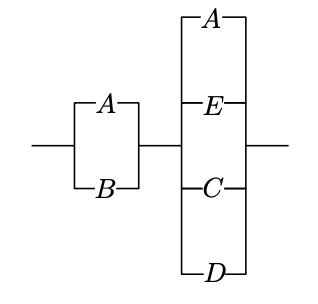
\includegraphics{vez1}
\end{center}
\noindent (ii)
\begin{center}
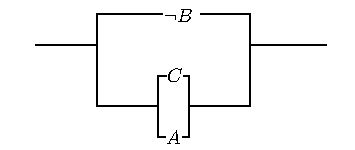
\includegraphics{vez2}
\end{center}
\noindent (iii)
\begin{center}
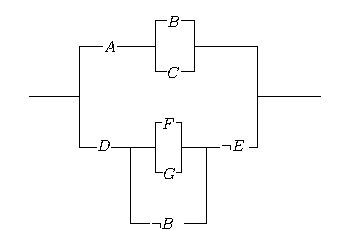
\includegraphics{vez3}
\end{center}




\item Simplify the following logical equivalence
$$(A\Rightarrow B) \vee (B \Rightarrow C).$$

\emph{Re"sitev.} 
\begin{eqnarray*}
(A\Rightarrow B) \vee (B \Rightarrow C) &\Leftrightarrow & (\neg A \vee B) \vee (\neg B \vee C)\\
&\Leftrightarrow & \neg A \vee B \vee \neg B \vee C\\
&\Leftrightarrow & \neg A \vee (B \vee \neg B) \vee C\\
&\Leftrightarrow & \neg A \vee 1 \vee C\\
&\Leftrightarrow & 1.
\end{eqnarray*}

\item Show that the following propositions are logical implications (a tautology where the main connective is implication).
\begin{enumerate}
\item[(i)] $A \wedge (A \Rightarrow B) \Rightarrow B$
\item[(ii)] $\neg B \wedge (A \Rightarrow B) \Rightarrow \neg A$
\item[(iii)] $\neg A \wedge (A \vee B) \Rightarrow B$
\item[(iv)] $(A \Rightarrow B) \wedge (B \Rightarrow C) \Rightarrow (A \Rightarrow C)$
\item[(v)] $A \wedge (A \Leftrightarrow B) \Rightarrow B$
\end{enumerate}

\emph{Re"sitev.} (i) Recimo $A \wedge (A \Rightarrow B)$ pravilna, $B$ pa nepravilna. Potem je $A$ pravilna in $A\Rightarrow B$ pravilna. Sledi $B$ pravilna. Protislovje. 


\item Are the following propositions logical implications?
\begin{enumerate}
\item[(i)] $(A \Rightarrow B ) \wedge (A \Rightarrow C) \wedge A \Rightarrow B \wedge C$
\item[(ii)] $\neg (A \vee B) \wedge (A\vee C) \wedge (D\Rightarrow C) \Rightarrow D$
\item[(iii)] $(A\Rightarrow B) \wedge (A\Rightarrow C) \wedge (D\wedge E \Rightarrow F) \wedge (C\Rightarrow E) \Rightarrow F$
\end{enumerate}

\item Z direktnim dokazom implikacije poka"zi: "Ce je $n$ sodo "stevilo, potem je $n^2 +3n$ sodo. Ali je obrat pravilen? 

\item Z direktnim dokazom implikacije poka"zi: "Ce je realno "stevilo $x$ nenegtivno, potem je vsota  "stevila $x$  in njegove obratne vrednosti  ve"cja ali enaka $2$.


\emph{ Re"sitev.} Poka"zimo $x + \frac{1}{x}\geq 2$. Ker $x\geq 0$, pomno"zimo neenakost z $x$ in dobimo
$x^2 + 1 \geq 2x$ oziroma $(x- 1)^2\geq 0$. Slednje je o"citno vedno res.

\item S protislovjem poka"zi, da je pra"stevil neskon"cno.

\emph{ Re"sitev.} Recimo, da jih je kon"cno mnogo $p_1,p_2,\ldots, p_n$. Potem  $p=p_1p_2\cdots p_n+1$ ni deljivo z nobenim pra"stevilom $p_i$ in $p_i\neq p$ za vsak $i$. Po definiciji je torej $p$ pra"stevilo, ki ni enako nobenemu prej"snjemu. Protislovje.

\item Poi"s"ci napako v naslednjem dokazu. 

\textbf{Trditev:} $1$ je najve"cje naravno "stevilo. 

\textbf{Dokaz} (s protislovjem):
Predpostavimo nasprotno. Naj bo $n>1$ najve"cje naravno "stevilo. Ker je $n$ pozitivno, lahko neenakost $n>1$ pomno"zimo z $n$. Torej $n>1\Leftrightarrow n^2>n$. Dobili smo, da je $n^2$ ve"cje od $n$, kar je v protislovju s predpostavko, da je $n$ najve"cje naravno "stevilo. Torej je bila predpostavka napa"cna in je $1$ najve"cje naravno "stevilo.

\emph{ Re"sitev.} Nasporotna trdtev je: obstaja naravno "stevilo, ki je ve"cje od $1$.


\item Naj bosta $x$ in $y$ realni "stevili, da velja $x<2y$. Z indirektnim dokazom poka"zi: "Ce je $7xy\leq 3x^2 + 2y^2$, potem je $3x\leq y$.

\emph{ Re"sitev.} Naj bo $x<2y$, to je, $2y-x>0$. Pokazali bomo: "ce je $3x> y$, potem je $7xy > 3x^2 + 2y^2$. Predpostavimo torej, da je $3x-y>0$. Potem je $(2y-x)(3x-y)= 7xy - 3x^2 - 2y^2>0$, to je, $7xy > 3x^2 + 2y^2$.

\item Doka"zi naslednjo ekvivalenco v dveh delih: Naj bosta $m$ in $n$ celi "stevili. Tedaj sta "stevili $m$ in $n$ razli"cnih parnosti natanko tedaj, ko je "stevilo $m^2- n^2$ liho.

\emph{ Re"sitev.} ($\Rightarrow$) Predpostavimo, da sta razli"cnih parnosti. Pi"simo  $m=2k$ in $n=2l+1$, vstavimo v izraz $m^2- n^2$ in rezultat sledi.

($\Leftarrow$) Poka"zemo indirektno in sicer: "Ce sta $m$ in $n$ iste parnosti, potem je $m^2- n^2$ sodo. Obravnavaj oba primera.


\item Z uporabo "ce in samo "ce dokaza poka"zi: $ac\,|\,bc \Leftrightarrow a\,|\,b$.

\item Ali je naslednji sklep pravilen?
\begin{enumerate}
\item[(i)] "Ce je danes sreda bom imel vaje. Danes je sreda. Sklep: Imel bom vaje.

\emph{ Re"sitev.} $(A\Rightarrow B) \wedge A \Rightarrow B$. Res je.

\item[(ii)] "Ce se u"cim, bom opravil izpit. Nisem se u"cil. Sklep: Ne bom opravil izpita.

\emph{ Re"sitev.} $(A\Rightarrow B) \wedge \neg A \Rightarrow \neg B$. Ni nujno res.
\end{enumerate}

\item Ali je naslednji premislek pravilen?
\begin{enumerate}
\item[(i)] "Student se je z mestni avtobusom odpravil na izpit. Rekel si je: "Ce bo na naslednjem semaforju zelena lu"c, bom naredil izpit. No, ko je avtobus pripeljal na naslednji semafor, na semaforju ni svetila zelena lu"c, "student pa si je dejal: Presneto, spet bom padel.

\emph{ Re"sitev.} $((A\Rightarrow B) \wedge \neg A) \Rightarrow \neg B$. Ni nujno res.

\item[(ii)] In"zenir, ki obvlada teorijo, vedno na"crta dobro vezje. Dobro vezje je ekonomi"cno. Torej, in"zenir, ki na"crta neekonomi"cno vezje, ne obvlada teorije. 

\emph{ Re"sitev.} $((A\Rightarrow B) \wedge (B\Rightarrow C)) \Rightarrow (\neg C \Rightarrow \neg A)$. Res je.
\end{enumerate}





\item Which of the following propositions are correct where the language of the conversation are real numbers?
\begin{enumerate}
\item[(i)] $(\forall x)(\exists y)(x+y=0)$.
\item[(ii)] $(\exists x)(\forall y)(x+y=0)$.
\item[(iii)] $(\exists x)(\exists y)(x^2+y^2 =-1)$.
\item[(iv)] $(\forall x)[x>0 \Rightarrow (\exists y)(y<0 \wedge xy>0)]$.
\end{enumerate} 




\item Let $A = \{ x \in \mathbb{N}; x < 7\}, B = \{x \in  \mathbb{Z}; |x - 2| < 4\}$ and $C = \{x \in\mathbb{R}; x^3 -  4x = 0\}$.
\begin{enumerate}
\item[(i)]  Write down the elements for all three sets.
\item[(ii)] Find $A \cup C, B \cap C, B \setminus C, (A \setminus B) \setminus C$ and $A \setminus (B \setminus C)$.
\end{enumerate}

\item Let  $\mathbb{Z}$ be a universal set and let  $P$ denote the set of all prime numbers, and $S$ the set of all even integers. Write the following propositions in terms of set theory:
\begin{itemize}
\item[(i)] There exists an even prime number. \quad [$P\cap S \neq \emptyset$]
\item[(ii)] $0$ is an integer, but it is not natural number. \quad [$0 \in \mathbb{Z}\setminus \mathbb{N}$]
\item[(iii)] Every natural number is an integer. \quad [$\mathbb{N}\subseteq \mathbb{Z}$]
\item[(iv)] Not every integer is a natural number. \quad [$\mathbb{Z}\nsubseteq \mathbb{N}$]
\item[(v)] Every prime number except 2 is odd. \quad [$P\setminus \{2\} \subseteq \overline{S}$]
\item[(vi)] 2 is an even prime number. \quad [$2\in S\cap P$]
\end{itemize}

\item Let  $A, B, C$ and $D$  be subsets of some universal set  $U$. Simplify the following expression
$$\overline{(\overline{(A\cup B)} \cap \overline{(\overline{A} \cup C)})}\setminus \overline{D}.$$

\item Show that $(A\cup C)\cap (B\setminus C) = (A\cap B)\setminus C$.

\emph{ Re"sitev.} 
\begin{eqnarray*}
x\in (A\cup C)\cap (B\setminus C) &\Leftrightarrow & (x\in A \vee x\in C) \wedge (x\in B \wedge x\notin C)\\
 &\Leftrightarrow & ((x\in A \vee x\in C) \wedge (x\notin C))\wedge x\notin B\\
&\Leftrightarrow & ((x\in A \wedge x\notin C) \vee (x\in C \wedge x\notin C)) \wedge
 x\in B\\
&\Leftrightarrow & x\in A \wedge x\notin C  \wedge x\in B\\
&\Leftrightarrow & x\in A \wedge x\in B  \wedge x\notin C \\
&\Leftrightarrow & x \in (A\cap B)\setminus C. 
\end{eqnarray*}

\item (Zadnja lastnost pri uniji) Prove that $A\subseteq C  \wedge B\subseteq C \Rightarrow A\cup B\subseteq C$.

\emph{ Re"sitev.} Direktno.

\item (Predzadnja lastnost pri preseku) Prove that $A\subseteq  B \Leftrightarrow A\cap B = A$.

\emph{ Re"sitev.} V dveh delih.

\item (Predzadnja lastnost pri kartezi"cnemu produktu) Prove that $A\times (B\cap C) = (A\times B)\cap (A\times C)$.

\emph{ Re"sitev.} 
\begin{eqnarray*}
(x,y)\in A\times (B\cap C) &\Leftrightarrow & x \in A \wedge y\in B\cap C\\
&\Leftrightarrow & x \in A \wedge y\in B  \wedge y\in C\\
&\Leftrightarrow & x \in A \wedge x \in A\wedge y\in B  \wedge y\in C\\
&\Leftrightarrow & x \in A \wedge  y\in B  \wedge x \in A\wedge y\in C\\
&\Leftrightarrow & (x,y) \in A\times B \wedge  (x,y) \in A\times C\\
&\Leftrightarrow & (x,y) \in (A\times B)\cap   (A\times C).
\end{eqnarray*}

\item (Predzadnja lastnost pri razliki) Prove that $(A\cap B )\setminus B = \emptyset$.
\emph{ Re"sitev.} 
\begin{eqnarray*}
x\in (A\cap B )\setminus B  &\Leftrightarrow & x \in (A\cap B)  \wedge x\notin B\\
&\Leftrightarrow & (x\in A\wedge x\in  B ) \wedge x\notin B\\
&\Leftrightarrow & x\in A\wedge (x\in  B  \wedge x\notin B)\\
&\Leftrightarrow & x\in \emptyset.
\end{eqnarray*}

\item Determine the following sets:
\begin{enumerate}
\item[(i)] $\{\emptyset, \{\emptyset\}\}\setminus \emptyset$ \quad [$\{\emptyset, \{\emptyset\}\}$]
\item[(ii)] $\{\emptyset, \{\emptyset\}\}\setminus \{\emptyset\}$
\item[(iii)] $\{\emptyset, \{\emptyset\}\}\setminus \{\}\emptyset\}\}$
\item[(iv)] $\{1,2,3,\{1\}, \{5\}  \}\setminus \{2,\{3\},5\}$
\end{enumerate}

\item Which of the following propositions are correct for arbitrary sets $A, B$ and $C$:
\begin{enumerate}
\item If $A\in B$ and $B\in C$, then $A\in C$.
\item If $A\subseteq B$ and $B\in C$, then $A\in C$.
\item If $A\cap B\subseteq \overline{C}$ and $A\cup C \subseteq B$, then $A\cap C = \emptyset$.
\item If $A\neq B$ and $B\neq C$, then $A\neq C$.
\item If $A\subseteq \overline{(B\cup C)}$ and $B\subseteq \overline{(A\cup C)}$, then $B=\emptyset$.
\end{enumerate}

\emph{ Re"sitev.}
\begin{enumerate}
\item Napa"cna. Vzemi $A=\emptyset$, $B=\{\emptyset\}$, $B=\{\{\emptyset\}\}$.
\item Napa"cna. Vzemi isti primer kot v (a).
\item Pravilna. Dokaz s protislovjem. Recimo, da trditev ni pravilna. Naj bo $A\cap B\subseteq \overline{C}$, $A\cup C\subseteq B$  in naj obstaja $x\in A\cap C$. Torej je $x\in A$ in $x\in C$. Ker je po drugi predpostavki $A\cup C\subseteq B$, je $x\in B$. Sledi $x\in A \cap B$. Ker je po prvi predpostavki $A\cap B\subseteq \overline{C}$, je $x\in \overline{C}$. Protislovje, saj $x\in C$. 
\item Napa"cna. Vzemi $A=C\neq B$.
\item Napa"cna. Vzemi tri paroma disjunktne neprazne mno"zice.
\end{enumerate}

\end{enumerate}

\chapter{Teorija množic}

\section{Množice}

{
\indent Množice so osnovni matematični objekti. Pojma množice ne definiramo.
Množice imajo elemente (ki so lahko tudi sami množice), običajno jih bomo označevali z malimi črkami:
$a,b,\ldots, x,y,z$ (+ indeksi: $a_6, x_1, z_\lambda$)

\smallskip

Množice pa bomo običajno pisali z velikimi črkami: $A,B,\ldots, X,Y,Z$ (+ indeksi)

\smallskip
Množice in elemente druži relacija pripadnosti:

$a\in F$: element $a$ \emph{ pripada} množici $F$, $a$ \emph{ je element} množice $F$.

\smallskip

$\in$: znak pripadnosti

\smallskip
$a\not\in F$: $a$ ni element (ne pripada) množici $F$.

\smallskip

\textbf{ Zgled:}
Če je $G$ množica vseh sodih števil, je $16\in G$ in $3\not\in G$.


\medskip
{\em Enakost množic:} Množici $A$ in $B$ sta enaki natanko takrat, kadar imata iste reči za elemente:

$$A = B \cee (\forall x) (x\in A\cee x\in B)$$

\medskip
Ta definicija je potrebna, saj podaja pomembno lastnost, ki ji mora relacija pripadnosti ustrezati!

\textbf{ Primer:} Recimo, da so objekti, ki jih preučujemo, ljudje,
in zapišimo $x\in A$ natanko tedaj, ko je $x$ prednik $A$-ja.
Ali lahko to definicijo uporabimo, da definiramo ljudi kot množice?
Zgornja ekvivalenca pravi:
\begin{itemize}
  \item {\em Če sta dva človeka enaka, potem imata iste prednike.} To drži.
  \item {\em Če imata dva človeka iste prednike, potem sta enaka.} To pa ne drži!
\end{itemize}

\noindent\textbf{ Načini podajanja množic:}
\begin{enumerate}
  \item Množico lahko podamo tako, da navedemo vse njene elemente:
$$A = \left\{1,\frac{1}{2}, \frac{\pi}{3}, 2i+8\right\}\,.$$
Vrstni red {\em ni pomemben!}
Včasih pa je ta zapis nepraktičen (kadar je množica neskončna ali pa končna, a prevelika).
  \item Množico lahko podamo tudi tako, da jo opišemo. Opis pa mora biti \textbf{ nedvoumen:}
za vsako reč mora veljati bodisi, da je element dane množice, ali pa da ni element te množice.

V splošnem lahko zapišemo:
$$A = \{x; P(x)\}\,,$$
kjer je $P(x)$ nek enomestni predikat.
{\em Množica $A$ je množica vseh elementov $x$, za katere je izjava $P(x)$ pravilna.}
Ali pa, če imamo več izjav $P_1,\ldots, P_n$:
$$A = \{x; P_1(x)\inn \cdots\inn P_n(x)\}$$
$$A = \{x; P_1(x)\ali \cdots\ali P_n(x)\}$$
Kot bomo kmalu videli, lahko take množice tvorimo le z elementi množic, ki jih že poznamo (oz.~za katere vemo, da obstajajo).
\end{enumerate}
}

\iftoggle{long}{\komentar{Večinoma skrajšano: DO TU}\\}

\begin{example*} Naj bo $A$ množica vseh takih kompleksnih števil $x$, ki so rešitev kakšne enačbe oblike
$$a_nx^n+a_{n-1}x^{n-1}+\cdots+a_1x+a_0 = 0\,,$$
kjer je $n\in \mathbb{N}$ in $a_i\in \mathbb{Z}$ za vse $i= 0,1,\ldots, n$.

\medskip
$A$ - množica vseh algebraičnih števil.

Ali je $2^{\pi}\in A$? Ne vemo (današnja matematika še ne more odgovoriti na to vprašanje).\end{example*}

%\begin{itemize}
%  \item Kadar je množica neskončna (npr.~množica vseh praštevil).
%  \item Kadar je množica končna, a prevelika (npr.~množica vseh knjig, ki so bile natisnjene na Zemlji do leta $2014$).
%\end{itemize}

%\medskip
%\textbf{ Zgled:}
%Naj bo $L$ množica vseh ljudi. Izjavi ``$x$ je poročen''~in ``$x$ je star vsaj 20 let''~sta smiselni izjavi za elemente množice $L$. Torej lahko tvorimo množice
%
%      $$\{x\in L; x \textrm{ je poročen}\}$$
%      $$\{x\in L; x \textrm{ je poročen} \inn x \textrm{ je star vsaj 20 let}\}$$

%pa tudi (z negacijo zgornje konjunkcije)
%      $$\{x\in L; x \textrm{ ni poročen} \ali x \textrm{ ni star vsaj 20 let}\}$$
%
%Množica
%      $$\{x\in L; x \textrm{ je sedanji predsednik Republike Slovenije}\}$$
%pa vsebuje samo Boruta Pahorja in ničesar drugega.

Pozor: škatla, ki vsebuje klobuk, ni ista reč kot klobuk. Tako tudi množica
$\{a\}$ ni ista reč kot $a$. Za vsako reč $a$ pa velja $a\in \{a\}$.


\subsection{Podmnožice}
Dani sta množici $A$ in $B$.

Pravimo, da je $A$ {\em podmnožica} množice $B$ natanko takrat, ko je vsak element množice $A$ tudi element množice $B$.

Oznaka: $A\subseteq B$

$$A\subseteq B\cee (\forall x)(x\in A\sledi x\in B)$$

Seveda je vsaka množica podmnožica same sebe: $$(\forall A)(A\subseteq A)\,.$$

 Če je $A\subseteq B$ in $A\neq B$, potem je $A$ {\em prava podmnožica} množice $B$: $A\subset B$.

$$A\subset B\cee (A\subseteq B \inn A\neq B)$$

Očitno velja:
\begin{itemize}
  \item $A\subseteq B \inn B\subseteq A \cee A = B$.
% Dokaz že pri Analizi 1.

  Ta ekvivalenca je izjemno pomembna za dokazovanje enakosti dveh množic!
  \item $A\subseteq B \inn B\subseteq C \sledi A \subseteq C \textrm{~(tranzitivnost inkluzije)}$
\end{itemize}

%Za dokaz ekvivalence $A\subseteq B \inn B\subseteq A \cee A = B$
%bomo privzeli naslednjo ekvivalenco:
%$$(\forall x)(P(x)\inn Q(x))\cee (\forall x)P(x)\inn (\forall x)Q(x)\,.$$
%(Dokaz na vajah.)

%\noindent\textbf{ Dokaz:}
%
%$(\Rightarrow)$:
%
%Dokazujemo s protislovjem.
%Recimo, da velja $(\forall x)(P(x)\inn Q(x))$, vendar pa
%
%$\neg((\forall x)P(x)\inn (\forall x)Q(x))\,.$
%
%Sledi:
%$\neg(\forall x)P(x)\ali \neg (\forall x)Q(x)\,.$
%
%$(\exists  x)\neg P(x)\ali (\exists x)\neg Q(x)\,.$
%
%Ne glede na to, katera od izjav $(\exists  x)\neg P(x)$
%in $(\exists  x)\neg Q(x)$ je pravilna, pridemo do protislovja z izjavo
%$(\forall x)(P(x)\inn Q(x))$.
%
%$(\Leftarrow)$:
%
%
%Dokazujemo s protislovjem.
%Recimo, da velja
%$(\forall x)P(x)\inn (\forall x)Q(x)\,,$ vendar pa
%
%$\neg (\forall x)(P(x)\inn Q(x))$.
%
%Sledi:
%$(\exists  x)\neg (P(x)\inn Q(x))$.
%
%$(\exists  x)(\neg P(x)\ali \neg Q(x))$.
%
%Naj bo $x$ tak, da velja $\neg P(x)\ali \neg Q(x)$.
%Ne glede na to, katera od izjav $\neg P(x)$ in
%$\neg Q(x)$ je pravilna, pridemo do protislovja z izjavo
%$(\forall x)P(x)\inn (\forall x)Q(x)\,.$\qed
%
%\bigskip
%Dokažimo sedaj ekvivalenco
%$$A\subseteq B \inn B\subseteq A \cee A = B\,:$$

%$$A\subseteq B \inn B\subseteq A$$
%$$\cee$$
%$$(\forall x)(x\in A\sledi x\in B) \inn (\forall x)(x\in B\sledi x\in A)$$
%$$\cee$$
%$$(\forall x)((x\in A\sledi x\in B) \inn (x\in B\sledi x\in A))$$
%$$\cee$$
%$$(\forall x)(x\in A\cee x\in B)$$
%$$\cee$$
%$$A = B\,.$$\qed
%
%

Dokažimo tranzitivnost inkluzije: $A\subseteq B \inn B\subseteq C \sledi A \subseteq C$

{\em Direkten dokaz:}

Privzemimo, da je $A\subseteq B$ in $B\subseteq C$.
Dokazati moramo: $(\forall x)(x\in A\sledi x\in C)$.

Vzemimo poljuben $x\in A$.
\begin{itemize}
  \item Ker je $x\in A$ in $A\subseteq B$, sledi $x\in B$.
  \item Ker je $x\in B$ in $B\subseteq C$, sledi $x\in C$.
\end{itemize}
Ker je bil $x$ poljuben, smo dokazali $(\forall x)(x\in A\sledi x\in C)$, tj., $A\subseteq C$.\qed


\medskip
\noindent\textbf{ V razmislek:} Ali obstajata množici $A$ in $B$, za kateri velja $A\subset B$ in $B\subset A$?

\bigskip
\noindent\textbf{ Pozor:} Relacija inkluzije $\subseteq$ in relacija pripadnosti $\in$ sta povsem različna pojma!

$1\in\{1,2,3\}$, toda $1$ ni podmnožica množice $\{1,2,3\}$.
Množica $\{1\}$ pa je podmnožica množice $\{1,2,3\}$, toda
$\{1\}$ ni element množice $\{1,2,3\}$.

\bigskip
\noindent\textbf{ V razmislek:} Naj bo $X = \{1,2,\{1\},\{2\}\}$.
Ali je $1$ element množice $X$?
Ali je $1$ podmnožica množice $X$?
Ali je $\{1\}$ element množice $X$?
Ali je $\{1\}$ podmnožica množice $X$?

\bigskip
\subsection{Prazna množica}
Množico, ki nima nobenega elementa, označimo s simbolom $\emptyset$ --- {\em prazna množica}.

$$X = \emptyset \cee (\forall x)(x\not\in X)$$

Seveda velja:
$$(\forall X) (\emptyset \subseteq X)$$

\textbf{ Domača naloga:} Dokažite, da velja:
$$X = \emptyset\cee (\forall Y)(X\subseteq Y)\,.$$

\subsection{Unija}

Dani sta množici $A$ in $B$. {\em Unija} teh dveh množic je množica $A\cup B$, ki ima za elemente natanko tiste reči, ki so elementi množice $A$ ali množice $B$:
$$A\cup B = \{x; x\in A \ali x\in B\}\,.$$

\textbf{ Zgled:}
$A = \{1,3,5,7\}$, $B = \{1,2,4,8\}$.

$A\cup B = \{1,3,5,7,2,4,8\}$.

\medskip
Posplošimo sedaj pojem unije dveh množic na unijo poljubne družine množic.
$A\cup B$ je unija družine množic $\{A,B\}$.
Tvorimo lahko množice množic (oziroma družine množic).

\begin{example*}
$\mathbb{Q}$: množica racionalnih števil je množica množic:
$$0,5 = \left\{\frac{1}{2}, \frac{2}{4}, \frac{3}{6}, \cdots\right\}$$
(Ulomek razumemo kot urejen par celih števil. Urejen par $(a,b)$ pa lahko, kot bomo videli kmalu, definiramo kot množico $\{\{a\},\{a,b\}\}$.)\end{example*}

\medskip

\textbf{ Unija več množic}:

V splošnem lahko družino množic zapišemo na naslednji način:

${\cal A} = \{A_\lambda; \lambda \in J\}$ - družina množic z indeksno množico $J$

Indeksna množica je poljubna množica!

\medskip
\begin{example*}
Za $J = \{1,2\}$ dobimo

${\cal A} = \{A_\lambda; \lambda \in \{1,2\}\} = \{A_1,A_2\}$.\end{example*}

\medskip
Unijo družine ${\cal A}$ definiramo kot
$$\cup {\cal A} = \cup_{\lambda \in J} A_\lambda = \{x;(\exists \lambda) (\lambda \in J\inn x\in A_\lambda)\}$$

\medskip
\begin{example*} $J = \{1,2\}$
$$\cup_{\lambda \in \{1,2\}} A_\lambda = \{x;(\exists \lambda) (\lambda \in \{1,2\}\inn x\in A_\lambda)\}= \{x;x\in A_1 \ali x\in A_2\} = A_1\cup A_2\,.$$
\end{example*}

\medskip
\begin{example*}
Vzemimo družino
${\cal A} = \{A_\lambda; \lambda \in J\}$, kjer je $J = \mathbb{Z}$ množica celih števil
in $A_\lambda = [\lambda,\lambda+1] = \{x; x\in \mathbb{R}~\inn~\lambda\le x\le \lambda +1\}$ za vse $\lambda\in \mathbb{Z}$.
Tedaj je
$$\cup {\cal A} = \cup_{\lambda\in \mathbb{Z}}A_\lambda
= \{x;(\exists \lambda) (\lambda \in \mathbb{Z}\inn \lambda \le x\le \lambda +1)\} = \mathbb{R}\,,$$
saj vsako realno število leži med dvema zaporednima celima številoma.\end{example*}

\medskip
Če je $J$ končna, vzamemo po navadi $J = \{1,2,\ldots, n\}$ in pišemo
$$\cup {\cal A} = \cup_{j = 1}^nA_j = A_1\cup\cdots\cup A_n\,.$$


\bigskip
\textbf{ Osnovne lastnosti unije:}
\begin{itemize}
  \item $A\cup B = B\cup A$, komutativnost
  \item $(A\cup B)\cup C = A\cup (B\cup C)$, asociativnost
  \item $A\cup A = A$, idempotentnost
  \item $A\cup \emptyset = A$
  \item $A\subseteq A\cup B$, $B\subseteq A\cup B$
  \item $A\subseteq B\cee A\cup B = B$
  \item $A\subseteq C\inn B\subseteq C\sledi A\cup B \subseteq C$
\end{itemize}

\bigskip
Dokažimo lastnost
$$A\subseteq B\cee A\cup B = B\,:$$
\medskip
Ekvivalenco bomo dokazali tako, da dokažemo obratno ekvivalenco
$\neg(A\subseteq B)\cee \neg(A\cup B = B)\,:$
Izkaže se, da je ugodneje obravnati najprej negacijo izjave na desni.
$$\neg(A\cup B = B)$$
$$\cee$$
$$\neg((A\cup B \subseteq B)\inn (B \subseteq A\cup B))$$
$$\cee$$
$$\neg(A\cup B \subseteq B) \ali \neg(B \subseteq A\cup B) $$
$$\cee$$
$$\neg(A\cup B \subseteq B)$$
$$\cee$$
$$(\exists x)(x\in A\cup B\inn x\not\in B)$$
$$\cee$$
$$(\exists x)((x\in A \ali x\in B)\inn x\not\in B)$$
$$\cee$$
$$(\exists x)((x\in A \inn x\not\in B) \ali (x\in B \inn x\not\in B))$$
$$\cee$$
$$(\exists x)(x\in A \inn x\not\in B)$$
$$\cee$$
$$\neg(\forall x)(x\in A\sledi x\in B)$$
$$\cee$$
$$\neg(A\subseteq B)$$
\qed

\bigskip
\textbf{ Domača naloga:} Dokažite preostale lastnosti.
\bigskip

\subsection{Presek}
Dani sta množici $A$ in $B$. {\em Presek} teh dveh množic je množica $A\cap B$, ki ima za elemente natanko tiste reči, ki so elementi množice $A$ in množice $B$:
$$A\cap B = \{x; x\in A \inn x\in B\}\,.$$

\textbf{ Zgled:}
$A = \{1,3,5,7\}$, $B = \{1,2,4,8\}$.

$A\cap B = \{1\}$.

\medskip

\textbf{ Presek več množic}:

${\cal A} = \{A_\lambda; \lambda \in J\}$ - družina množic z indeksno množico $J$, $J\neq \emptyset$!

Indeksna množica je poljubna \textbf{ neprazna} množica!

Presek neprazne družine ${\cal A}$ definiramo kot
$$\cap {\cal A} = \cap_{\lambda \in J} A_\lambda = \{x;(\forall\lambda) (\lambda \in J\sledi x\in A_\lambda)\}$$
(Če bi bil $J = \emptyset$, bi $\cap {\cal A}$ = vse. To pa ni možno zaradi Russellove antinomije (ki ste jo že spoznali pri Analizi 1)!)

\medskip
Če je $J$ končna, vzamemo po navadi $J = \{1,2,\ldots, n\}$ in pišemo
$$\cap {\cal A} = \cap_{j = 1}^nA_j = A_1\cap\cdots\cap A_n\,.$$

Če velja
$A\cap B = \emptyset$, pravimo, da sta si množici $A$ in $B$ {\em tuji}
(ali da sta {\em disjunktni}).

\bigskip
\textbf{ Osnovne lastnosti preseka:}
\begin{itemize}
  \item $A\cap B = B\cap A$, komutativnost
  \item $(A\cap B)\cap C = A\cap (B\cap C)$, asociativnost
  \item $A\cap A = A$, idempotentnost
  \item $A\cap \emptyset = \emptyset$
  \item $A\cap B\subseteq A$, $A\cap B\subseteq B$,
  \item $A\subseteq B\cee A\cap B = A$
  \item $A\subseteq B\inn A\subseteq C\sledi A \subseteq B\cap C$
\end{itemize}

\bigskip
\textbf{ Domača naloga:} Dokažite te lastnosti. (Dokazi so podobni dokazom analognih lastnosti za unijo.)

\bigskip
Unija in presek sta povezana z distributivnostnima zakonoma:
$$(A\cup B)\cap C = (A\cap C)\cup (B\cap C)$$
$$(A\cap B)\cup C = (A\cup C)\cap (B\cup C)$$

Dokažimo prvi distributivnostni zakon:
$(A\cup B)\cap C = (A\cap C)\cup (B\cap C)$.

{\em Kako dokažemo enakost dveh množic, $X = Y$? Možnih je več načinov:
\begin{enumerate}
 \item Po definiciji. Torej
    direktno dokažemo pravilnost izjave $(\forall x)(x\in X\cee x\in Y)$.

    ALI

\item  S pomočjo ekvivalence $X = Y \Longrightarrow X\subseteq Y \inn Y\subseteq X$.
\begin{enumerate}
         \item   Dokažemo $X\subseteq Y$, tj., pravilnost izjave $(\forall x)(x\in X\sledi x\in Y)$.
 \item Dokažemo še $Y\subseteq X$, tj., pravilnost izjave $(\forall x)(x\in Y\sledi x\in X)$.
        \end{enumerate}
        \end{enumerate}}

Poglejmo si 1.~način:
$$x\in (A\cup B)\cap C$$
$$\cee$$
$$(x\in A\cup B) \inn (x\in C)$$
$$\cee$$
$$(x\in A\ali x\in B) \inn (x\in C)$$
$$\cee$$
$$(x\in A \inn  x\in C)\ali (x\in B \inn  x\in C) $$
$$\cee$$
$$(x\in A \cap C)\ali (x\in B \cap C) $$
$$\cee$$
$$x\in (A \cap C)\cup (B \cap C)\,.$$
Ker gornja veriga ekvivalenc velja za poljuben $x$, je izjava
$$(\forall x)(x\in (A\cup B)\cap C\cee x\in (A \cap C)\cup (B \cap C))$$
pravilna. Torej sta množici enaki.
\qed

Distributivnostna zakona veljata tudi bolj splošno, za neprazne družine množic:
$$(\bigcup_{\lambda\in J}A_\lambda)\cap (\bigcup_{\mu\in K}B_\mu) =
\bigcup_{\lambda\in J, \mu\in K}(A_\lambda\cap B_\mu)\,.$$
$$(\bigcap_{\lambda\in J}A_\lambda)\cup (\bigcap_{\mu\in K}B_\mu) =
\bigcap_{\lambda\in J, \mu\in K}(A_\lambda\cup B_\mu)\,.$$

\medskip
\textbf{ Domača naloga:} Dokažite, da za poljubne tri množice $A$, $B$, $C$ velja:
$$(A\cap B)\cup C = A\cap (B\cup C) \cee C\subseteq A\,.$$
(Pogoj na desni je neodvisen od množice $B$!)

%\subsection*{Ponovitev:}
%Zadnjič smo začeli z obravnavo množic.
%
%Relaciji pripadnosti $\in$ in inkluzije $\subseteq$. Podmnožica, prazna množica, Russellova antinomija, urejeni par, unija.
%
%\medskip
%Relaciji pripadnosti in inkluzije sta povezani takole:
%$$(\forall x)(\forall X)(x\in X\cee \{x\}\subseteq X)\,.$$
%
%$\{a\}\cup \{\{a\}\} = \{a,\{a\}\}$
%
%$\{a\}\cup \{b\} = \{a,b\}\neq \{\{a\},\{b\}\}$
%
%$\{a\}\cup \{b\}\cup \{c\} = \{a,b,c\}$
%
\bigskip

Ponovimo: Unijo družine množic ${\cal A} = \{A_\lambda; \lambda \in J\}$ smo definirali kot\\
$\cup {\cal A} = \{x;(\exists \lambda) (\lambda \in J\inn x\in A_\lambda)\}$, presek neprazne družine množic pa kot \\
\hbox{$\cap {\cal A} = \{x;(\forall \lambda) (\lambda \in J\sledi x\in A_\lambda)\}$.}

Kaj dobimo v primeru ${\cal A} = \{A_1\}$? $J= \{1\}$.
$$\cup \{A_1\}
= \{x;(\exists \lambda) (\lambda \in \{1\}\inn x\in A_\lambda)\}
= \{x;(\exists \lambda) (\lambda = 1 \inn x\in A_\lambda)\}
 = \{x;x\in A_1\} = A_1\,.$$
$$\cap \{A_1\} =
\{x;(\forall \lambda) (\lambda \in \{1\}\sledi x\in A_\lambda)\}
= \{x;(\forall \lambda)(\lambda= 1\sledi x\in A_\lambda)\}
 = \{x;x\in A_1\} = A_1\,.$$

Pisano brez indeksov: $\cup \{A\} = \cap \{A\} = A$.

Podobno velja tudi $\cup \{\emptyset\} = \cap \{\emptyset\} = \emptyset$ in $\cup \emptyset = \emptyset$.


\subsection{Razlika množic}

Dani sta množici $A$ in $B$.

{\em Razlika} množic $A$ in $B$ je množica, ki ima za elemente natanko tiste reči, ki so elementi množice $A$, niso pa elementi množice $B$.
$$A\brez B = \{x; x\in A\inn x\not\in B\}\,.$$

\textbf{ Zgled:}
Naj bo $A$ množica praštevil, $B$ pa množica vseh pozitivnih lihih števil.
Tedaj je

$A\brez B = \{2\}$ (2 je edino sodo praštevilo)

$B\brez A = \{1,9,15,21,25,\ldots\}$ (množica vseh lihih števil, ki niso praštevila)

\bigskip

Osnovne lastnosti:

\begin{itemize}
  \item $A\brez A = \emptyset$

  \item $A\brez (A\cap B) = A\brez B$

  \item $A\cap (A\brez B) = A\brez B$

  \item $A\brez (B\cup C) = (A\brez B)\cap (A\brez C)$

  \item $A\brez (B\cap C) = (A\brez B)\cup (A\brez C)$

  \item $(A\brez B)\cup B = A\cup B$

  \item $(A\cup B)\brez B = A\brez B$

  \item $(A\cap B)\brez B = \emptyset$

  \item $(A\brez B)\cap B = \emptyset$
\end{itemize}

Dokažimo enakost $(A\brez B)\cup B = A\cup B$:

$$x\in (A\brez B)\cup B$$
$$\cee$$
$$x\in A\brez B \ali x\in B$$
$$\cee$$
$$(x\in A\inn x\not\in B) \ali x\in B$$
$$\cee$$
$$(x\in A\ali x\in B) \inn (x\not\in B \ali x\in B)$$
$$\cee$$
$$(x\in A\ali x\in B)$$
$$\cee$$
$$x\in A\cup B$$
\qed

%\newpage
\bigskip
\textbf{ Domača naloga:} Dokažite preostale lastnosti.

\bigskip
%konec 3. predavanj (T4)



\bigskip

Zelo pogosto smo v matematiki v temle položaju: podana je neka {\em univerzalna množica} $S$, zanimamo se izključno za elemente in podmnožice množice $S$.

Naj bo $A\subseteq S$. Tedaj lahko definiramo {\em komplement množice $A$ (glede na množico $S$)} kot:
$$C_SA = \overline A = S\brez A\,.$$
Če množice $S$ ne definiramo, ne moremo govoriti o komplementu: $\overline \emptyset$ = množica vseh množic --- ta pa ne obstaja (Russellova antinomija)!

\bigskip
%\newpage
\begin{example*}
Naj bo $S = \{0,1,2,3,\ldots\}$ množica naravnih števil, množica $A$ pa množica praštevil.
Potem je $\overline A = \{0,1,4,6,8,9,10,12,\ldots\}$.

\end{example*}

\medskip

Lastnosti komplementa:
\begin{itemize}
  \item
$\overline S = \emptyset,~~~~\overline \emptyset = S$

  \item
$\overline{\overline A} = A,~~~A\cup \overline A = S,~~~~A\cap \overline A = \emptyset$

  \item
$A\brez B = A\cap \overline B$

  \item
$A\subseteq B \cee  \overline B \subseteq \overline A$

  \item
$A= B \cee  \overline A = \overline B$

  \item
$\overline{A\cup B} = \overline A\cap \overline B$,~~~$\overline{A\cap B} = \overline A\cup \overline B$ (De Morganova zakona)
\end{itemize}

De Morganova zakona veljata tudi za poljubno družino množic ${\cal A} = \{A_\lambda~;~\lambda\in J\}$:
$$\overline{\cup_{\lambda\in J}A_\lambda} = {\cap_{\lambda\in J}\overline A_\lambda}$$
$$\overline{\cap_{\lambda\in J}A_\lambda} = {\cup_{\lambda\in J}\overline A_\lambda}$$

Zaradi De Morganovih zakonov se izreki v teoriji množic pogosto pojavljajo v parih.
Če v neki inkluziji, enakosti ali ekvivalenci o unijah, presekih in komplementih podmnožic neke množice zamenjamo vsako množico z njenim komplementom,
zamenjamo vse unije in preseke in obrnemo vse inkluzije, je rezultat spet neka veljavna inkluzija, enakost ali ekvivalenca. Temu principu pravimo \textbf{ princip dualnosti}.

%\newpage

\bigskip
\begin{example*}

Trditev
$$(A\cap B)\cup C = A\cap (B\cup C) \cee C\subseteq A\,.$$
postane
$$(\overline A\cup \overline B)\cap \overline C = \overline A\cup (\overline B\cap \overline C) \cee \overline A\subseteq \overline C\,,$$
kar je ekvivalentno trditvi
$$(A\cup B)\cap C = A\cup (B\cap C) \cee A\subseteq C$$
(zamenjali smo vloge množic in njihovih komplementov).
\end{example*}

%\newpage
\subsection{Vennovi diagrami}

Vse odnose in operacije med podmnožicami dane univerzalne množice lahko nazorno prikažemo s t.i.~{\em Vennovimi diagrami}.


\begin{center}
\includegraphics[width=111mm]{Venn.eps}
\end{center}

\medskip
Seveda pa tako ``slikanje'' nima nobene zveze z dokazovanjem.

%\newpage
\subsection{Potenčna množica}

{\em Potenčna množica} dane množice $A$ je družina množic, ki ima za svoje elemente natanko podmnožice množice $A$:
$${\cal P}(A) = \{X; X\subseteq A\}$$

\textbf{ Zgled:}
\begin{itemize}
  \item ${\cal P}(\{1,2\}) = \{\emptyset, \{1\},\{2\},\{1,2\}\}$
  \item ${\cal P}(\emptyset) = \{\emptyset\}$.
  \item ${\cal P}(\{\emptyset\}) = \{\emptyset, \{\emptyset\}\}$.
\end{itemize}

Če ima množica $A$ $n$ elementov, potem ima njena potenčna množica ${\cal P}(A)$ $2^n$ elementov.\footnote{Za vsakega od $n$ elementov množice $A$ je potrebno določiti, neodvisno od ostalih, ali ga množica $X\subseteq A$ vsebuje ali ne. Skupaj imamo torej $n$ neodvisnih izbir ene izmed dveh možnosti, kar nam da, za vse podmnožice $X\subseteq A$, ravno $2^n$ možnosti.}

\bigskip
Lastnosti:
\begin{itemize}
  \item $A\subseteq B\sledi \P(A) \subseteq \P(B)$.
  \item $\P(A) \cup \P(B) \subseteq \P(A\cup B)$.
  \item $\P(A)\cap \P(B) =  \P(A\cap B)$.
\end{itemize}

Prva lastnost sledi iz tranzitivnosti inkluzije:

$X\in \P(A) \inn A\subseteq B\cee X\subseteq A\subseteq B\sledi X\subseteq B\cee X\in \P(B)$.

Dokaz druge lastnosti:

$X\in \P(A) \cup \P(B) \cee X\subseteq A\ali X\subseteq B\sledi X\subseteq A\cup B\cee X\in \P(A\cup B)$.


Dokaz tretje lastnosti:

$X\in \P(A)\cap \P(B)\cee X\in \P(A) \inn A\in \P(B)\cee X\subseteq A \inn X\subseteq B$

$\cee X\subseteq A \cap B\cee X\in \P(A\cap B)$

%\textbf{ V razmislek:} Zakaj velja predzadnja ekvivalenca v zgornji verigi ekvivalenc?
%
%\medskip
%\textbf{ Domača naloga:} Formalno dokažite prvo in drugo lastnost.

\medskip
\textbf{ V razmislek:} Ali v prvi lastnosti velja ekvivalenca?

\medskip
\textbf{ V razmislek:} Zakaj v drugi lastnosti ne velja enakost?


\subsection{Urejeni par}

Vzemimo dve reči $a$ in $b$.
%$a\neq b$.

Za množico $\{a,b\}$ vrstni red ni pomemben, $\{a,b\} = \{b,a\}$.

Kadar je vrstni red pomemben, govorimo o {\em urejenem paru}:

$(a,b)$ - urejen par, $(a,b)\neq (b,a)$

$a$ - prva koordinata

$b$ - druga koordinata

Kdaj sta dva urejena para enaka?
$$(a,b) = (u,v) \cee a = u \inn b = v\,.$$

\medskip
Urejeni par $(a,b)$ definiramo kot množico $\{\{a\},\{a,b\}\}$.

\medskip
\textbf{ Domača naloga:}
Dokažite, da velja $\{\{a\},\{a,b\}\} = \{\{u\},\{u,v\}\}\cee a = u \inn b = v\,.$



\subsection{Kartezični produkt}

Pojem kartezičnega produkta ste spoznali že pri Analizi I.

{\em Kartezični produkt} množic $A$ in $B$ je množica, ki ima za elemente natanko vse urejene pare $(x,y)$, kjer je prva koordinata iz množice $A$, druga koordinata pa iz množice $B$:
$$A\times B = \{(x,y)~;~x\in A\inn y\in B\}$$



\textbf{ Zgled:} $\{1\}\times \{2,3\} = \{(1,2),(1,3)\}$,

$\{2,3\}\times \{1\} = \{(2,1),(3,1)\}$.

\bigskip
Lastnosti kartezičnega produkta:
\begin{itemize}
  \item $A\times B\neq B\times A$ (razen če je $A = B$)
  \item $A\times B = \emptyset \cee A= \emptyset \ali B = \emptyset$.
  \item $A\times (B\cup C) = (A\times B) \cup (A\times C)$.
  \item $A\times (B\cap C) = (A\times B) \cap (A\times C)$.
  \item $A\times (B\brez C) = (A\times B) \brez (A\times C)$.
\end{itemize}

Kartezični produkt treh množic definiramo kot:

$$A\times B\times C = (A\times B)\times C= \{((x,y),z)~;~x\in A \inn y\in B\inn z\in C\}\,.$$

Po navadi pišemo kar: $((x,y),z) = (x,y,z)$ (urejena trojica).

\bigskip
Kartezični produkt množic $A_1,\ldots, A_n$ definiramo kot
množico vseh urejenih $n$-teric:
$$A_1\times A_2\times\cdots \times A_n = \prod_{i = 1}^n A_i = \{(x_1,\ldots, x_n)~;~x_1\in A_1\inn x_2\in A_2\inn\cdots \inn x_n\in A_n\}\,.$$
Če so vsi faktorji enaki, $A_1 = A_2 = \ldots,  = A_n = S$, dobimo {\em $n$-kratni kartezični produkt množice $S$ s samo seboj},
$$S^n = \Pi_{i = 1}^nS = S\times\cdots\times S~~\textrm{$n$ faktorjev}\,.$$

\begin{example*}
Če je $S = \mathbb{R}$ množica realnih števil,
dobimo za $n = 2$ množico točk v ravnini~($\mathbb{R}^2$), za
$n = 3$ pa množico točk v prostoru ($\mathbb{R}^3$).\end{example*}

\bigskip

%Dokažimo še enega od De Morganovih zakonov za poljubno družino množic ${\cal A} = \{A_\lambda~;~\lambda\in J\}$:
%$$\overline{\cup_{\lambda\in J}A_\lambda} = {\cap_{\lambda\in J}\overline A_\lambda}$$
%
%$$x\in \overline{\cup_{\lambda\in J}A_\lambda}
%\cee
%x\not\in \cup_{\lambda\in J}A_\lambda
%\cee
%\neg(\exists \lambda)(\lambda \in J\inn x\in A_\lambda)
%\cee$$
%$$\cee(\forall \lambda)(\lambda \in J\sledi \neg(x\in A_\lambda))
%\cee
%(\forall \lambda)(\lambda \in J\sledi x\in \overline{A_\lambda})
%\cee
%x\in {\cap_{\lambda\in J}\overline A_\lambda}\,.$$
%
\bigskip
\textbf{ Rešitev dveh domačih nalog:}

Dokažimo, da za poljubne tri množice $A$, $B$, $C$ velja:
$$(A\cap B)\cup C = A\cap (B\cup C) \cee C\subseteq A\,.$$

\medskip
$(\Rightarrow)$:
Naj bo $(A\cap B)\cup C = A\cap (B\cup C)$.

$C\subseteq (A\cap B)\cup C = A\cap (B\cup C)\subseteq A$. Uporabimo tranzitivnost inkluzije.

\medskip
$(\Leftarrow)$:
Naj bo $C\subseteq A$. Tedaj je $A\cup C = A$.

Torej je
$(A\cap B)\cup C = (A\cup C)\cap (B\cup C) = A\cap (B\cup C)$.

\bigskip
Dokažimo implikacijo
$$A\subseteq C\inn B\subseteq C\sledi A\cup B \subseteq C\,:$$

Dokaz s protislovjem:
$$\neg(A\cup B\subseteq C)$$
$$\cee$$
$$(\exists x)(x\in A\cup B\inn x\not\in C)$$
$$\cee$$
$$(\exists x)((x\in A \ali x\in B)\inn x\not\in C)$$
$$\cee$$
$$(\exists x)((x\in A \inn x\not\in C) \ali (x\in B\inn x\not\in C))$$
$$\cee$$
$$(\exists x)((x\in A \inn x\not\in C) \ali (x\in B\inn x\not\in C))$$
$$\cee$$
$$(\exists x)(x\in A \inn x\not\in C) \ali (\exists x)(x\in B\inn x\not\in C)$$
$$\cee$$
$$\neg(\forall x)(x\in A\sledi x\in C)\ali\neg(\forall x)(x\in B\sledi x\in C)$$
$$\cee$$
$$\neg(A \subseteq C) \ali \neg(B\subseteq C)$$
$$\cee$$
$$\neg(A \subseteq C \inn B\subseteq C)\,.$$
\qed

Dokazali smo ne samo implikacijo, ampak ekvivalenco
$$A\subseteq C\inn B\subseteq C\cee A\cup B \subseteq C\,.$$


\section{Na kratko o aksiomih}

Vsaka matematična teorija temelji na množici aksiomov --- osnovnih trditev, ki jih {\em privzamemo} za pravilne. Ti aksiomi opredeljujejo osnovne lastnosti, ki jim morajo zadoščati objekti obravnavane teorije (npr.~naravna števila, realna števila, grupe, vektorski prostori, topološki prostori, ...) Iz aksiomov pa potem s pomočjo logičnega sklepanja izpeljujemo nove resnice, ki jim pravimo trditve, posledice, izreki.

V teoriji množic ni nič drugače! Obstaja več družin aksiomov, najbolj pa je uveljavljenih 7 aksiomov, imenovanih {\em aksiomi ZFC} (Zermelo--Fraenkel--(Axiom of) Choice).

Aksiomi zagotavljajo obstoj množic in tvorjenje novih množic iz že obstoječih.
%Razen aksioma izbire, ki je posebnega pomena, drugih aksiomov tu ne bomo podrobneje obravnavali.

Da bi razumeli, zakaj potrebujemo aksiome, si poglejmo, zakaj množica vseh
množic ne obstaja.

\subsection{Russellova antinomija}

Ali obstaja {\em množica vseh množic?}

Recimo, da obstaja. Naj bo $A$ množica vseh množic.

Za vsako množico se lahko vprašamo, ali ima samo sebe za element. $\mathbb{N}$ nima same sebe za element! Množica vseh abstraktnih pojmov pa ima samo sebe za element.

Naj bo $B\subseteq A$ tista podmnožica množice $A$, ki ima za elemente natanko tiste množice iz $A$, ki nimajo same sebe za element.

Ali ima množica $B$ samo sebe za element?

Če ja, potem nima same sebe za element!

Kaj pa če $B$ nima same sebe za element? Potem pa po definiciji $B\in B$.
Protislovje.

{\em Množica vseh množic ne obstaja!}

{\centerline\em Nič ne vsebuje vsega.} \textit{(Matematično) vesolje ne obstaja.}

\medskip
Torej pri oblikovanju množic ne smemo preveč zaupati svoji intuiciji. Potrebni so aksiomi, ki zagotavljajo obstoj nekaterih množic.
 %(npr.~aksiom o paru, aksiom o uniji, aksiom o podmnožici, itd.).

\subsection{Aksiomi teorije množic (po Endertonu)}

\begin{enumerate}
  \item Aksiom o ekstenzionalnosti (enakost množic)
  $$\forall A\, \forall B\, (\forall x \,(x\in A \cee x\in B) \sledi A = B)$$

  \item Aksiom o prazni množici:
  \emph{ Obstaja prazna množica.}
  $$\exists B\, \forall x\, (x\not \in B)$$

  \item Aksiom o paru: \emph{ Obstajajo dvoelementne množice.}
    $$\forall u\, \forall v\, \exists B\, \forall x\, (x\in B \cee x = u\textrm{ ali }x = v)$$

  \item Aksiom o uniji: \emph{ Obstaja unija poljubne družine množic.}
    $$\forall A\, \exists B\, \forall x\, (x\in B \cee (\exists b\in A) x\in b)$$

  \item Aksiom o potenčni množici: \emph{ Obstaja potenčna množica vsake množice.}
    $$\forall a\, \exists B\, \forall x (x\in B \cee x\subseteq a)$$

  \item Aksiomska shema o podmnožicah: \emph{ Obstajajo raznovrstne podmnožice.}

  Za vsako predikatno formulo $\varphi$ o množicah $t_1,\ldots, t_k$, ki ne vsebuje črke $B$, je naslednji izraz aksiom:
$$\forall t_1\,\cdots\, \forall t_k\,\forall c\,\exists B \,\forall x \,(x\in B \cee x\in c \inn \varphi)$$

\begin{example*}
(Za $k = 1$):

$\forall a \,\forall c \,\exists B \, \forall x\, (x\in B \cee x\in c \inn x\in a)$

To pomeni, da za vsaki dve množici $a$ in $c$ obstaja množica $B = a\cap c$, njun presek.
\end{example*}
\medskip
Zgornja aksiomska shema omogoča opisovanje množic v obliki
$$\{x\in A; P(x)\}\,.$$

\begin{example*}
$\{x\in \mathbb{R}; x\ge 0\}$.
\end{example*}

  \item Aksiom o neskončnosti: \emph{ Obstaja neskončna množica.}
$$\exists A\,(\emptyset \,\in A \inn (\forall a\in A)\, (a\cup \{a\}\in A))$$

\item Aksiom izbire: \emph{ Vsaka relacija vsebuje funkcijo z isto domeno.}
$$(\forall \textrm{ relacijo }R)(\exists \textrm{ funkcija }F)(F\subseteq R \inn {\cal D}(F) = {\cal D}(R))$$
Ta aksiom bomo podrobno obravnavali v poglavju 2.5.

%\item Aksiomska shema o zamenjavi: \emph{ Zaloga vrednosti vsake funkcije je množica.}

%Ta aksiomska shema omogoča opisovanje množic v obliki
%$$\{f(x); x\in A\}\,,$$
%kjer je $f$ neka funkcija z domeno $A$.

%Na ta način lahko zapišemo množico $\{x^2; x\in \mathbb{R}\}$. Ta je enaka množici $\{x\in \mathbb{R}; x\ge 0\}$.

%Za vsako formulo $\varphi(x,y)$, ki ne vsebuje črke $B$,
%je naslednji izraz aksiom:
%$$\forall t_1\,\cdots \forall t_k\,\forall A\,[(\forall x\in A)\,\forall y_1\, \forall y_2\, (\varphi(x,y_1) \inn \varphi(x,y_2) \sledi y_1 = y_2)$$
%$$\sledi \exists B\, \forall y\, [y\in B \cee (\exists x\in A)\,\varphi(x,y)]$$

%\item Aksiom regularnosti: \emph{ Vsaka neprazna množica vsebuje element, ki je z njo disjunkten.}
%$$(\forall A\neq \emptyset)\,(\exists m\in A)\,(m\cap A = \emptyset)$$

%Ta aksiom med drugim zagotovi, da ne obstajata množici $A$ in $B$, za kateri bi veljalo $A\in B$ in $B\in A$.
%(Kot poseben primer, za $A = B$, dobimo, da nobena množica ni element same sebe.)
\end{enumerate}

Nekatere aksiome oz.~aksiomske sheme, in sicer 2., 3.~in 6.~z zgornjega seznama, je moč izpeljati iz preostalih 7 aksiomov.

\section{Pregled najpomembnejših pojmov in nekaj nalog}

Ključni pojmi:
\begin{itemize}
  \item Relacija pripadnosti. Enakost množic.
  \item Presek in unija družine množic. Distributivnost. Razlika dveh množic, komplement.
  \item Podmnožica, relacija inkluzije. Prava podmnožica. Prazna množica.
  \item Russellova antinomija.
  \item De Morganova zakona, princip dualnosti.
  \item Potenčna množica. Kartezični produkt.
\end{itemize}

\begin{problem}[Enakost množic]
Katere naslednjih množic so med seboj enake?
$$\{r,s,t\}, \{t,r,s,t\}, \{s,s,r,r,t\}, \{t,s,r\}$$
\end{problem}

Odgovor: Vse.

\bigskip
\begin{problem}
Ali obstajajo take množice $A, B, C$, da velja $B\neq C$ in $A\cap B = A\cap C$?
\end{problem}

Odgovor: Da: lahko vzamemo npr.~$A = \emptyset$ in poljubni različni množici $B\neq C$
(potem bo namreč $A\cap B = A\cap C = \emptyset$).

Ali pa: $A = \{1,2\}, B = \{2,3\}, C = \{2,4\}$.


\begin{problem}
Dana je množica $A$. Poišči vse množice $B$, za katere velja
$A\backslash B = B\backslash A$.
\end{problem}

\textbf{Rešitev:}

\textbf{1.~ način}:

Očitno je
$(A\backslash B) \cap (B\backslash A)=\emptyset$.
Ob upoštevanju predpostavke $A\backslash B = B\backslash A$
zveza
$(A\backslash B) \cap (B\backslash A)=\emptyset$
postane
$A\backslash B =\emptyset$
in $B\backslash A =\emptyset$, kar pomeni
$A\subseteq B$ in $B\subseteq A$. Torej je $B = A$.\qed

\textbf{2.~ način}:

$A\backslash B = B\backslash A \sledi(A\cap B)\cup (A\backslash B) = (B\cap A)\cup (B\backslash A) \sledi A = B$.\qed

\begin{problem}
Drži ali ne drži?

Za poljubne množice $A$, $B$ in $C$ velja:
$$A\cup (B\times C) = (A\cup B)\times (A\cup C)\,.$$
\end{problem}

Ne drži. Že zato, ker množica na levi strani ni nujno kartezični produkt dveh množic.

Zgled: $A = \{1\}, B = C = \emptyset$.




\chapter{Relacije}

%\textbf{ \color{red}Na vajah je bilo v redu. Delali smo naloge iz mnozic. Naredili smo tudi tri priemre,
%ki so bili za domaco nalogo in sicer zadnjo lastnost pri uniji in predzadnjo lastnost pri preseku ter
%razliki.}

%\medskip
Znotraj vsake matematične teorije ${\cal T}$ z univerzalno množico $S$
lahko vsako smiselno lastnost $P(x)$ predstavimo z množico
$$\{x~;~x\in S\inn P(x)\}\,.$$
Tudi odnose ali {\em relacije} moremo predstaviti z množicami.

\medskip
Primeri dvomestnih (binarnih) relacij: $\in$, $\subseteq$, $=$, $\le$, $>$, vzporeden, skladen
\begin{itemize}
          \item Primer: 3 in 5 sta v relaciji ``manjši".
\end{itemize}
Trimestne relacije: vsota, razlika, produkt

------

``Družinske'' relacije: oče, sin, mati, sestra, mož, tašča, $\ldots$

starši - trimestna relacija ($x,y,z$ so v relaciji natanko tedaj, ko sta $x$ in $y$ starša $z$)

\section{Splošno o relacijah}

Naj bo $R$ neka smiselna binarna relacija za neko matematično teorijo ${\cal T}$ z univerzalno množico $S$.

$R$ bomo predstavili z množico natanko tistih urejenih parov množice $S$,
katerih prva koordinata je v relaciji $R$ z drugo koordinato.

$x$ je v relaciji $R$ z $y$: $xRy$ ali $R(x,y)$.
$$R = \{(x,y)~;~x,y\in S\inn xRy\}$$
ali krajše (če se razume, kaj je univerzalna množica $S$):
$$R = \{(x,y)~;~xRy\}\,.$$

\medskip
Če je $R$ $n$-mestna relacija, pa uporabimo $n$-terice:
$$R = \{(x_1,\ldots, x_n)~;~R(x_1,\ldots, x_n)\}$$

------

Dvomestna relacija je torej \textbf{ podmnožica kartezičnega produkta} $S\times S =: S^2$.

$n$-mestna relacija pa je podmnožica $n$-kratnega kartezičnega produkta množice $S$ s samo seboj, $S^n$.


\bigskip
\begin{example*}

$S = \{1,2,3,4\}$,

Dvomestna relacija ``manjši'', $<(x,y) \cee x<y$:

$$< = \{(1,2),(1,3),(1,4), (2,3), (2,4), (3,4)\}\,.$$

Trimestna relacija ``vsota'', $+(x,y,z) \cee x+y = z$:

$$+ = \{(1,1,2),(1,2,3),(1,3,4), (2,1,3), (2,2,4), (3,1,4)\}\,.$$
\end{example*}

\bigskip

% 11. predavanje: 16.11.2011, 2 uri

\begin{example*}

$S = \{1,2,3,4,5,6\}$,

Dvomestna relacija $R$ ``je večkratnik'', $R(x,y) \cee x$ je večkratnik $y$, tj.,

$(\exists k)(k$ je pozitivno naravno število in $x = k\cdot y$):
$$R = \{(1,1),(2,1),(2,2),(3,1),(3,3),(4,1),(4,2),(4,4),(5,1),(5,5),(6,1),(6,2),(6,3),(6,6)\}\,.$$

Trimestna relacija ``produkt'', $\cdot(x,y,z) \cee z = x\cdot y$:
$$\cdot  = \{(1,1,1),(1,2,2),(1,3,3),(1,4,4),(1,5,5),(1,6,6),(2,1,2),$$$$(2,2,4),(2,3,6),(3,1,3),(3,2,6),(4,1,4),(5,1,5),(6,1,6)\}\,.$$


Enomestna relacija ``praštevilo'', $P(x) \cee x$ je praštevilo:

$P = \{2,3,5\}$.
\end{example*}

\bigskip

Ker smo relacije predstavili z množicami, lahko govorimo tudi o relacijah
$R\cup T$, $R\cap T$, $R\brez T$ (če sta relaciji $R$ in $T$ obe $n$-mestni relaciji za isti $n$).

\bigskip
\begin{example*}
Če z $R_{\leq}$, $R_{<}$, $R_{=}$, $R_{\ge}$, $R_{>}$ in $R_{\neq}$
zaporedoma označimo relacije ``manjši ali enak'', ``manjši'', ``enak'',
``večji ali enak'', ``večji'' in ``neenak'' (npr.~na množici naravnih števil), potem velja:
%$$(x\leq  y) = (x<y) \cup (x = y)$$
%$$(x> y) = (x\ge y) \brez (x = y)$$
%$$(x> y) = (x\ge y) \cap (x \neq y)$$
$$R_\leq = R_< \cup R_=$$
$$R_> = R_\ge \brez R_= = R_\ge \cap R_{\neq}$$
\end{example*}


Osredotočimo se sedaj na \textbf{ binarne relacije} (te so posebnega pomena, kot bomo videli v poglavju o strukturah urejenosti).

Naj bo $R$ binarna relacija v univerzalni množici $S$:
$$R = \{(x,y)~;~xRy\}\,.$$

Množico vseh prvih koordinat elementov iz $R$ imenujemo {\em domena relacije $R$.}

Množico vseh drugih koordinat elementov iz $R$ pa imenujemo {\em zaloga vrednosti (kodomena) relacije $R$.}

Domena: $${\cal D}R = \{x~;~(\exists y)(xRy)\}$$
Zaloga vrednosti: $${\cal Z}R = \{y~;~(\exists x)(xRy)\}$$
(v uporabi sta tudi oznaki ${\cal R} R$ in $\textrm{Im} R$)

\medskip

\begin{example*}

$R = \{(1,2), (2,3), (2,4)\}$.

${\cal D}R = \{1,2\}$,

${\cal Z}R = \{2,3,4\}$

\end{example*}

 \begin{example*}
Naj bo $X$ poljubna množica in $S = X\cup {\cal P}(X)$. Relacija $R$ je podmnožica $S\times S$, definirana s predpisom
$$xRy\cee x\in X\inn y\in {\cal P}(X) \inn x\in y\,.$$
Tedaj je ${\cal D}R = X$ in ${\cal Z}R = {\cal P}(X)\brez \{\emptyset\}\,.$
\end{example*}


\subsection{ Inverzna relacija}
$$R^{-1}= \{(y,x)~;~xRy\}$$
Očitno je:
\begin{itemize}
  \item $yR^{-1}x \cee xRy\,.$
  \item ${\cal D}R^{-1} = {\cal Z}R$ in ${\cal Z}R^{-1} = {\cal D}R$.
    \item $(R^{-1})^{-1} = R$.
\end{itemize}


\bigskip
\begin{example*}

 $R_\le^{-1}~~=~~R_\ge\,,$

 $R_<^{-1}~~=~~R_>\,,$

 $R_=^{-1}~~=~~R_{\neq}\,,$


$R_{\neq}^{-1}~~=~~R_{\neq}\,.$\end{example*}


\subsection{Kompozitum relacij}

Dani sta binarni relaciji $R$ in $T$.

$T\circ R$: kompozitum relacije $R$ z relacijo $T$

$$x T\circ R y \cee (\exists u)(xRu\inn uTy)$$

$$T\circ R = \{(x,y)~;~(\exists u)(xRu\inn uTy)\}$$

Očitno velja: $T\circ R\subseteq ({\cal D}R)\times ({\cal Z}T)$.

\bigskip
\begin{example*}

$R = \{(1,3),(2,3)\}$, $T = \{(3,1), (2,1)\}$

$R\circ T = \{(1,1), (2,1)\}$, 
$T\circ R = \{(3,3),(2,3)\}$.

\medskip

brat $\circ$ oče $\subseteq$ oče

oče  $\circ$ brat $\subseteq$ stric

(oče $\circ$ brat)$\cup$(mati $\circ$ brat) = stric

sestra $\circ$ mati $\subseteq$  mati

(žena $\circ$ mati) $\cup$ (mož $\circ$ mati) = tašča
\end{example*}

\medskip
Torej v splošnem $T\circ R\neq R\circ T$. Velja pa asociativnost.

% konec predavanj - 8.11.2018

\begin{trditev}
Naj bodo $V, T, R$ binarne relacije v univerzalni množici $S$. Tedaj velja
$$V\circ(T\circ R) = (V\circ T)\circ R\,.$$
\end{trditev}

\begin{proof}
$$(x,y)\in V\circ(T\circ R)\cee x V\circ(T\circ R) y
\cee$$
$$(\exists u)(x(T\circ R)u\inn uVy)
\cee (\exists u)(\exists v)(xRv\inn vTu\inn uVy)\cee $$
$$(\exists v)(xRv\inn (\exists u)(vTu\inn uVy))
\cee(\exists v)(xRv\inn v(V\circ T)y)\cee$$
$$x ((V\circ T)\circ R)y \cee (x,y)\in (V\circ T)\circ R\,.$$
\end{proof}

Inverz kompozituma je enak kompozitumu inverzov v obratnem vrstnem redu:

\begin{trditev}
Naj bosta $T$ in $R$ binarni relaciji v univerzalni množici $S$. Tedaj velja
$$(T\circ R)^{-1} = R^{-1}\circ T^{-1}\,.$$
\end{trditev}

\begin{proof}
$$(x,y)\in (T\circ R)^{-1} \cee (y,x)\in T\circ R
\cee$$
$$(\exists u)(yRu\inn uTx)
\cee (\exists u)(uR^{-1}y\inn xT^{-1}u)
\cee$$
$$(\exists u)(xT^{-1}u\inn uR^{-1}y)
\cee x (R^{-1}\circ T^{-1}) y\cee (x,y)\in R^{-1}\circ T^{-1}\,.$$
\end{proof}


\bigskip
\begin{example*}

Naj bosta $a,b\in\mathbb{R}$.

Definirajmo relaciji

$R = \{(x,y)~;~x+y = a\}$,

$T = \{(x,y)~;~x+y = b\}$.

Tedaj je

$T\circ R = \{(x,y)~;~(\exists u)(x+u = a\inn u+y = b)\}=\{(x,y)~;~x-y = a-b\}$.

$R\circ T = \{(x,y)~;~x-y = b-a\}$.

$R^{-1}= R$, $T^{-1} = T$.

Enakost v zgornji trditvi v tem primeru postane
$(T\circ R)^{-1} = R \circ T\,.$
\end{example*}

%\bigskip
%Rešimo dve nalogi o množicah.
%
%\medskip
%
%1.~Pokazali smo, da velja ${\cal P}(A)\cup {\cal P}(B)\subseteq  {\cal P}(A\cup B)$.
%
%Dokaži, da velja
%$${\cal P}(A)\cup {\cal P}(B)={\cal P}(A\cup B)$$
%natanko tedaj, ko je $$(A\subseteq B) \ali (B\subseteq A)\,.$$.
%
%\bigskip
%${\cal P}(A)\cup {\cal P}(B)={\cal P}(A\cup B)$
%
%$\cee$
%
%${\cal P}(A\cup B) \subseteq {\cal P}(A)\cup {\cal P}(B)$
%
%$\cee$
%
%$(\forall X)(X\in {\cal P}(A\cup B)\sledi X\in {\cal P}(A)\cup {\cal P}(B))$
%
%$\cee$
%
%$(\forall X)(X\subseteq A\cup B\sledi X\subseteq A \ali X\subseteq B)$
%
%$\cee$
%
%$(A\subseteq B) \ali (B\subseteq A)$
%
%\bigskip
%Dokaz zadnje ekvivalence napravimo posebej:
%
%$(\Leftarrow)$:
%Če je $(A\subseteq B) \ali (B\subseteq A)$, potem je
%$A\cup B = B \ali A\cup B = A$ in v vsakem primeru velja
%$(\forall X)(X\subseteq A\cup B\sledi X\subseteq A \ali X\subseteq B)$.
%
%\medskip
%
%$(\Rightarrow)$:
%Recimo, da je
%$(\forall X)(X\subseteq A\cup B\sledi X\subseteq A \ali X\subseteq B)$
%in da ne velja
%$(A\subseteq B) \ali (B\subseteq A)$.
%
%Torej je
%$\neg((A\subseteq B) \ali (B\subseteq A))$
%
%$\sledi$
%
%$\neg(A\subseteq B) \inn \neg(B\subseteq A)$
%
%$\sledi$
%
%$(\exists a)(a\in A\brez B)\inn (\exists b)(b\in B\brez A)$.
%
%Tedaj pa za množico $X = \{a,b\}$ velja $X\subseteq A\cup B$, vendar ne velja $X\subseteq A$ niti $X\subseteq B$.
%Protislovje.\hfill\qed
%
%\bigskip
%2.~Dokažimo ekvivalenco
%$$A\subseteq B\cee A\cap B = A\,.$$
%
%\medskip
%$(\Leftarrow)$: $A=A\cap B\subseteq B$.
%
%\medskip
%$(\Rightarrow)$:
%Naj bo $A\subseteq B$.
%
%Pokazati moramo: $(A\cap B\subseteq A)\inn(A\subseteq A\cap B)$.
%
%$A\cap B\subseteq A$ vselej velja.
%
%Dokažimo relacijo $A\subseteq A\cap B$ s protislovjem.
%
%Recimo, da
%$(\exists x)(x\in A\inn x\not\in A\cap B)$.
%
%$\sledi (\exists x)(x\in A\inn \neg(x\in A \inn x\in B))$
%
%$\sledi (\exists x)(x\in A\inn (x\not\in A \ali x\not \in B))$
%
%$\sledi (\exists x)((x\in A\inn x\not\in A) \ali (x\in A\inn x\not \in B))$
%
%$\sledi (\exists x)(x\in A\inn x\not \in B)$
%
%$\sledi \neg (\forall x)(x\in A\sledi x\in B)$
%
%To pa je protislovje s predpostavko $A\subseteq B$.

% ŠE DVE NALOGI:
% 1. definicija (a,b) je dobra
% 2. kartezični produkt in razlika

\subsection{Univerzalna, ničelna in identična relacija}

V vsaki množici $S$ imamo tri posebne relacije:

$S\times S$ -- univerzalna relacija

$\emptyset$ -- ničelna relacija

$I = \{(x,x)~;~x\in S\}$ -- identična relacija (relacija identitete)

\begin{trditev}
Naj bo $R$ binarna relacija v univerzalni množici $S$.

Tedaj velja $I\circ R = R\circ I = R$.
\end{trditev}

\begin{proof}
$xI\circ Ry \cee (\exists u)(xRu \inn uIy) \cee xRy$.

$xR\circ Iy \cee (\exists u)(xIu \inn uRy) \cee xRy$.
\end{proof}

\medskip
Velja tudi:

\begin{itemize}
  \item $\emptyset \circ R = R\circ \emptyset = \emptyset$
  \item $(S\times S)\circ R =
({\cal D}R) \times S$ in $R\circ (S\times S) = S\times {\cal Z}R$.
\end{itemize}

Dokažimo enakost $R\circ (S\times S) = S\times {\cal Z}R$:

$x(R\circ (S\times S))y \cee (\exists u)(x(S\times S)u \inn uRy)
\cee (\exists u)(uRy) \cee y\in {\cal Z}R \cee x\in S\inn y\in {\cal Z}R  \cee x(S\times {\cal Z}R)y$.

\bigskip

\textbf{ Domača naloga}: Dokažite enakost
$(S\times S)\circ R = ({\cal D}R) \times S$.

%$x((S\times S)\circ R)y \cee (\exists u)(x R u \inn u(S\times S)y)
%\cee (\exists u)(xRu) \cee x\in {\cal D}R \cee x\in {\cal D}R\inn y\in S  \cee x(({\cal D}R) \times S)y$.

\section{Posebne lastnosti binarnih relacij}

Nekatere lastnosti binarnih relacij so še posebej pomembne:

\bigskip

$R \textrm{ je {\em refleksivna}} \cee (\forall x)(x\in S\sledi xRx)$

%\begin{center}
%\includegraphics[height=20mm]{refleksivna.eps}
%\end{center}

\textbf{ Zgled:} relacija $\le$ v realnih številih

\bigskip

$R \textrm{ je {\em irefleksivna}} \cee (\forall x)(x\in S\sledi \neg(xRx))$

%\begin{center}
%\includegraphics[height=20mm]{irefleksivna.eps}
%\end{center}

\textbf{ Zgled:} relacija $<$ v realnih številih

\bigskip

$R \textrm{ je {\em simetrična}} \cee (\forall x)(\forall y)(x\in S\inn y\in S\inn xRy\sledi yRx)$

%\begin{center}
%\includegraphics[height=20mm]{simetricna.eps}
%\end{center}
%
\textbf{ Zgled:} vzporednost premic


\bigskip

$R \textrm{ je {\em asimetrična}} \cee (\forall x)(\forall y)(x\in S\inn y\in S\inn xRy\sledi \neg(yRx))$

%\begin{center}
%\includegraphics[height=20mm]{asimetricna.eps}
%\end{center}

\textbf{ Zgled:} relacija $<$ v realnih številih

% 12. predavanje, 2 uri, 22. 11. 2011

\bigskip
$R \textrm{ je {\em antisimetrična}} \cee (\forall x)(\forall y)(x\in S\inn y\in S\inn xRy\inn yRx\sledi x = y)$

\textbf{ Zgled:}
relacija $\le$ v realnih številih

relacija $\subseteq$ v množicah

\bigskip

$R \textrm{ je {\em tranzitivna}} \cee (\forall x)(\forall y)(\forall z)(x\in S\inn y\in S\inn z\in S\inn xRy\inn yRz\sledi xRz)$

%\begin{center}
%\includegraphics[height=20mm]{tranzitivna.eps}
%\end{center}

\textbf{ Zgled:} relacija $<$ v realnih številih

relacija $\subset$ v množicah

\bigskip

$R \textrm{ je {\em intranzitivna}} \cee (\forall x)(\forall y)(\forall z)(x\in S\inn y\in S\inn z\in S\inn xRy\inn yRz\sledi \neg(xRz))$

%\begin{center}
%\includegraphics[height=20mm]{intranzitivna.eps}
%\end{center}

\textbf{ Zgled:}
relacija $R$ v realnih številih, definirana s predpisom $xRy \cee x = y + 1$

pravokotnost premic v ravnini

\bigskip

$R \textrm{ je {\em strogo sovisna}} \cee (\forall x)(\forall y)(x\in S\inn y\in S
\inn x\neq y\sledi (xRy)\ali (yRx))$

%\begin{center}
%\includegraphics[height=20mm]{sovisna.eps}
%\end{center}

\textbf{ Zgled:}
relacija $<$ v realnih  številih

\bigskip

$R \textrm{ je {\em sovisna}} \cee (\forall x)(\forall y)(x\in S\inn y\in S
\sledi (xRy)\ali (yRx))$

%\begin{center}
%\includegraphics[height=20mm]{strogosovisna.eps}
%\end{center}

\textbf{ Zgled:}

relacija $\le$ v realnih številih

\bigskip
\textbf{ Domača naloga:}
Izberite si nekaj sorodstvenih relacij in za vsako od njih ugotovite, katere od zgornjih lastnosti imajo.

\bigskip
Nekatere od zgornjih lastnosti niso med seboj neodvisne:
\begin{itemize}
  \item $R$ je strogo sovisna $\sledi$ $R$ je sovisna.
  \item $R$ je asimetrična $\sledi$ $R$ je irefleksivna.
  \item $R$ je simetrična in tranzitivna $\sledi$ $R$ je refleksivna (če je ${\cal D}R = S$).
\end{itemize}

\section{Ekvivalenčna relacija}

$R$ je {\em ekvivalenčna} $\cee$ $R$ je refleksivna, simetrična in tranzitivna.

\textbf{ Zgled:} relacija identitete

\bigskip
Ekvivalenčne relacije lahko karakteriziramo na naslednji način.

\begin{trditev}
$R$ je ekvivalenčna $\cee$ ${\cal D}R = S$ in $R^{-1}\circ R = R$.
\end{trditev}

\begin{proof}
Pogoj je potreben:

$xRx \sledi {\cal D}R = S$
$$xR^{-1}\circ Ry \sledi (\exists z)(xRz \inn zR^{-1}y)
\sledi (\exists z)(xRz \inn yRz)
\sledi (\exists z)(xRz \inn zRy)
\sledi xRy\,.$$
$$xRy
\sledi (xRy\inn yRy)
\sledi (xRy\inn yR^{-1}y)
\sledi xR^{-1}\circ Ry\,.$$
Torej $R^{-1}\circ R = R$.

Pogoj je pa tudi zadosten:

Naj bo ${\cal D}R = S$ in $R^{-1}\circ R = R$.

Refleksivnost: dokazujemo $(\forall x)(x\in S\sledi xRx)$.
Naj bo $x\in S$. Ker je ${\cal D}R = S$,
je $x\in {\cal D}R\sledi (\exists y)(y\in S\inn xRy)$.
$$xRy
\sledi xRy\inn yR^{-1}x
\sledi x R^{-1}\circ R x
\sledi xRx\,.$$

Simetričnost: dokazujemo $(\forall x)(\forall y)(x\in S\inn y\in S\inn xRy\sledi yRx)\,.$

Naj bo $x\in S\inn y\in S\inn xRy$.
Tedaj je
$$xRy \sledi (xRy\inn yRy)
\sledi (yRy\inn yR^{-1}x)
\sledi yR^{-1}\circ Rx
\sledi yRx\,.$$

Tranzitivnost: dokazujemo $(\forall x)(\forall y)(\forall z)(x\in S\inn y\in S\inn z\in S\inn xRy\inn yRz\sledi xRz).$

Naj bo $x\in S\inn y\in S\inn z\in S\inn xRy\inn yRz$.
Tedaj je
$$xRy \inn yRz \sledi xRy\inn zRy
\sledi xRy\inn yR^{-1}z
\sledi xR^{-1}\circ Rz
\sledi xRz\,.$$
\end{proof}

\medskip
Ekvivalenčna relacija ima to lepo lastnost, da razdeli množico $S$, na kateri je definirana, na {\em same neprazne in paroma disjunktne množice, katerih unija
je prav množica~$S$}.

\medskip
\textbf{ Ekvivalenčni razredi.}

Naj bo $R$ ekvivalenčna relacija, definirana v množici $S$. Naj bo $x\in S$. {\em Ekvivalenčni razred elementa $x$ glede na ekvivalenčno relacijo $R$} je množica vseh elementov, ki so v relaciji z $x$:
$$R[x] = \{y~;y\in S \inn yRx\}\,.$$

Za ekvivalenčne razrede velja naslednje:
\begin{itemize}
  \item Ker je $R$ refleksivna relacija, velja $x\in R[x]$. Posledično je $R[x]\neq \emptyset$.
  \item $y\in R[x]\sledi R[y]=R[x]$.

  Res: Naj bo $y\in R[x]$.

  $z\in R[y]\sledi zRy\inn yRx\sledi zRx\sledi z\in R[x]$.

  $z\in R[x]\sledi zRx\inn yRx\sledi zRx\inn xRy \sledi zRy\sledi z\in R[y]$.
  \item $y\not\in R[x]\sledi R[x]\cap R[y]=\emptyset$.

  Res: $(\exists z)(z\in R[x]\cap R[y])\sledi (\exists z)(R[z] = R[x]\inn R[z] = R[y])\sledi
  y\in R[y]=R[x]$. Protislovje z domnevo $y\not\in R[x]$.
  \end{itemize}

Sledi:
\begin{enumerate}
  \item Vsak element množice $S$ je v natanko enem ekvivalenčnem razredu. Namreč v tistem, v katerem so združeni vsi elementi množice $S$, ki so z njim v relaciji $R$.
  \item Vsak ekvivalenčni razred je povsem določen s poljubnim elementom, ki mu pripada. Zato pravimo, da je poljuben element danega razreda {\em predstavnik} tega razreda.
      \item Z ekvivalenčnimi razredi dane ekvivalenčne relacije $R$ je množica $S$
      razdeljena na same neprazne in paroma tuje podmnožice, katerih unija je množica $S$.
      \end{enumerate}


\begin{center}
\includegraphics[height=30mm]{ekvivalencna.eps}
\end{center}

Takim razdelitvam pravimo particije. {\em Particija množice $S$} = družina nepraznih in paroma disjunktnih množic, katerih unija je množica $S$.

Vsaki ekvivalenčni relaciji torej ustreza neka particija množice $S$.
Velja pa tudi obratno. Vsaka particija ${\cal A}$ množice $S$ določa natanko eno ekvivalenčno relacijo $R$, in sicer tako, da so množice v particiji ravno ekvivalenčni razredi glede na relacijo $R$:
\begin{itemize}
  \item Poljubna elementa $x$ in $y$ sta v relaciji $R$ natanko takrat, ko pripadata isti množici iz particije:
      $$xRy\cee (\exists X)(X\in {\cal A}\inn x\in X\inn y\in X)\,.$$
\end{itemize}
Premislimo, da je tako definirana relacija ekvivalenčna:
\begin{itemize}
  \item refleksivna: $x\in S \sledi (\exists X)(X\in {\cal A}\inn x\in X)\sledi xRx\,.$
  \item simetrična:
  $xRy\sledi (\exists X)(X\in {\cal A}\inn x\in X\inn y\in X)
  \sledi (\exists X)(X\in {\cal A}\inn y\in X\inn x\in X)\sledi yRx\,.$
  \item tranzitivna:
  $xRy \inn yRz\sledi (\exists X)(X\in {\cal A}\inn x\in X\inn y\in X)
  \inn (\exists Y)(Y\in {\cal A}\inn y\in Y\inn z\in Y)$.

  Torej je $y$ hkrati v množici $X$ in $Y$. Ker pa so množice paroma disjunktne, sledi
  $X = Y$. Potem pa je element $z$ tudi v množici $X$. Sledi $xRz$.
\end{itemize}

\textbf{ V razmislek:} Utemelji, da particija ${\cal A}$ sovpada z množico ekvivalenčnih razredov relacije $R$.

%
%\textbf{ Ponovitev:}
%
%binarne relacije
%
%domena
%
%zaloga vrednosti

%\medskip
%Inverzna relacija. Kompozitum relacij.
%
%$x(T\circ R)y \cee (\exists u)(xRu\inn uTy)$.
%
%$(R\circ T)^{-1} = T^{-1}\circ R^{-1}$
%
%ničelna relacija, identična relacija,
%univerzalna relacija
%
%\bigskip
%
%Rešitev domače  naloge:  $(S\times S)\circ R = ({\cal D}R) \times S$.
%
%\bigskip
%Obravnavali smo ekvivalenčne relacije:
%
%Relacija je ekvivalečna, če je refleksivna, simetrična in tranzitivna.
%
\medskip


% 14. predavanje, 2 uri, 29. 11. 2011

Vsaki množici $S$, v kateri je definirana kakšna ekvivalenčna relacija $R$, moremo prirediti neko novo množico, katere elementi so ekvivalenčni razredi relacije $R$:

{\em Faktorska množica množice $S$ glede na relacijo $R$}:
$$S/R = \{R[x]~;~x\in S\}=\{X~;~(\exists x)(x\in S \inn X = R[x])\}$$
\begin{itemize}
  \item Faktorska množica predstavlja matematično formulacijo logičnega principa {\em abstrakcije}: S tem ko iz dane množice $S$ preidemo na faktorsko množico, abstrahiramo vse razlike med rečmi, ki pripadajo istemu ekvivalenčnemu razredu!
\end{itemize}


\bigskip
\begin{example*}

Naj bo $S = \{1,2,3\}$ in $R = \{(1,1),(1,3),(2,2),(3,1),(3,3)\}$.

Relacija $R$ je ekvivalenčna.

$R[1] = R[3] = \{1,3\}$, $R[2] = \{2\}$.

$S/R =  \{R[1], R[2],R[3]\} = \{R[1], R[2]\} = \{\{1,3\},\{2\}\}$.

\v Ce definiramo particijo ${\cal A} = \{\{1,3\},\{2\}\}$ množice $S$, potem lahko definiramo relacijo $R'$ s predpisom
$xR'y \cee (\exists X)(X\in {\cal A}\inn x\in X\inn y\in Y)$.
Velja

$R' = \{(1,1),(1,3),(3,1),(2,2),(3,3)\} = R$
in $S/R' = \{\{1,3\},\{2\}\} = {\cal A}$.
\end{example*}


\subsubsection*{Zgledi ekvivalenčnih relacij}

\begin{enumerate}
  \item \textbf{ Ulomki.}

  V množici ulomkov $$a/b\,,$$
  kjer sta $a$ in $b$ poljubni celi števili in je $b\neq 0$, je definicija enakosti dveh ulomkov
  $$a/b = c/d \cee ad = bc$$
  očitno ekvivalenčna relacija. Vsak ekvivalenčni razred glede na to relacijo druži vse med seboj enake ulomke in predstavlja tedaj ustrezno {\em racionalno število}. Prirejena faktorska množica je {\em množica racionalnih števil}.
  \item \textbf{ Kongruence.}


  V množici {\em celih števil} je relacija {\em kongruence po modulu $m$}, kjer je $m> 0$ poljubno pozitivno celo število, $$a\equiv b \textrm{ (mod $m$)}\cee m \textrm{ deli }a-b\,,$$
  ekvivalenčna relacija.

  Ekvivalenčni razredi so v tem primeru {\em razredi ostankov} po modulu $m$. V vsakem ekvivalenčnem razredu so vsa tista števila, ki dajo pri deljenju z $m$ isti ostanek.

  Očitno je takih razredov natanko $m$. Te razrede imenujemo {\em cela števila po modulu $m$}. Faktorska množica je množica celih števil po modulu $m$.

  \item \textbf{ Vzporednost premic.}

V množici {\em vseh premic} je relacija ``vzporeden'' ekvivalenčna relacija. V vsakem ekvivalenčnem razredu so torej vse premice, ki so med seboj vzporedne, in predstavljajo potemtakem določeno {\em smer}. Faktorska množica je tukaj {\em množica vseh smeri}.
\end{enumerate}

\section{Funkcije}

{\em Funkcija je osrednji pojem klasične in moderne matematike. Od 18.~stoletja naprej
je pojem funkcije postajal vse bolj precizen in splošen. Definicijo funkcije, kot jo poznamo danes, sta uvedla Cauchy in Riemann:}

\medskip
%Znana je naslednja definicija:
Za dani množici $A$ in $B$ je {\em funkcija iz $A$ v $B$} predpis, ki vsakemu elementu množice $A$ priredi natanko določen element množice $B$.
Oznaka: $f:A\to B$.

\medskip
Da pa se izognemo dvomu, kaj je mišljeno z besedo ``predpis", funkcije lahko definiramo kot posebne vrste relacij.

\medskip
Binarna relacija $R$ je {\em enolična}, če velja:
$$(x,y)\in R \inn (x,z)\in R\sledi y = z$$

{\em Parcialna funkcija} je enolična binarna relacija. Parcialne funkcije navadno označujemo s črkami $f, g,h,\ldots$

\emph{ Funkcija, ki preslika množico $A$ v množico $B$} (ali krašje: {\em funkcija iz $A$ v $B$}), je taka parcialna funkcija $f$, da
velja
$${\cal D}f= A \textrm{~~~in~~~} (x,y)\in f\sledi x\in A\inn y\in B\,.$$
Oznaka: $f:A\to B$.

Funkcijam pravimo tudi {\em preslikave, upodobitve, transformacije}.
Množico vseh funkcij iz $A$ v $B$ označimo z $B^A$.

\bigskip

Pišemo
$$y=f(x)\cee (x,y)\in f\,.$$
$$f = \{(x,y)~;~x\in A\inn y = f(x)\in B\}\,.$$

$x\in A$: neodvisna spremenljivka, original, argument

$y (= f(x))$: odvisna spremenljivka, slika elementa $x$.

\medskip

V uporabi sta tudi oznaki

$x\mapsto f(x)$~~``$x$ se preslika v $f(x)$",

$A\overset{f}{\to} B$~~``$f$ preslika $A$ v $B$".

\bigskip
\textbf{ Zgledi funkcij:}
\begin{itemize}
  \item $A = \{1,2,3\}$, $B = \{2,4,6\}$

  $f = \{(1,2),(2,4),(3,4)\}$

  \item $A = \{$točke na površju planeta Zemlja$\}$, $B = \mathbb{R}$,

$f(x) = $ temperatura v $^\circ C$ v kraju $x$ dne $1.~1.~2015$ ob 6:00 po lokalnem času

  \item $A = \{$ljudje, živeči na Zemlji ob času $T\}$, $B = \mathbb{N}$,

$f(x) = $ starost (v sekundah) osebe $x$ v času $T$.
\end{itemize}

\bigskip
Množici $\{(x,y)~;~x\in A\inn y = f(x)\}$ včasih pravimo tudi {\em graf funkcije.}

\bigskip
\textbf{ Upodobitve funkcij.}
V primeru, ko je $A\subseteq \mathbb{R}$ in $B = \mathbb{R}$, lahko graf funkcije upodobimo kot množico točk v ravnini.

\textbf{ Zgled:} $f:\mathbb{R}\to \mathbb{R},~~~f(x) = x^2\,.$
\begin{center}
\includegraphics[height=50mm]{f.eps}
\end{center}

\medskip

Na enak način lahko upodobimo tudi {\em relacije} na množici  $S =\mathbb{R}$:

Naj bo $xRy \cee x^2+y^2 = 4$.
Tedaj relacijo $R$ predstavlja krožnica z radijem $2$ in s središčem v koordinatnem izhodišču.

\begin{center}
\includegraphics[height=50mm]{x2+y2=4.eps}
\end{center}

\bigskip
Naj bo $f:A\to B$. Domena funkcije $f$:
$${\cal D}f = \{x~;~(\exists y)((x,y)\in f)\} = A$$
Zaloga vrednosti funkcije $f$:
$${\cal Z}f = \{y~;~y\in B\inn (\exists x)(x\in A\inn (x,y)\in f)\} \subseteq B\,.$$
Množici $B$ pravimo \emph{ kodomena} funkcije $f$.

\medskip
\begin{example*}
Naj bo $f = \{(1,2),(2,4),(3,4)\}$, $A = \{1,2,3\}$, $B = \{2,4,6\}$.

Tedaj je ${\cal D}f = \{1,2,3\}$, ${\cal Z}f = \{2,4\}$.\end{example*}

\bigskip
Pri analizi ste obravnavali tudi realne funkcije, ki jih običajno podamo kar s predpisom $f(x)$, ne da bi navajali domeno in kodomeno.
Za domeno v tem primeru vzamemo množico $\{x\in \mathbb{R}; f(x)\in \mathbb{R}\}$, ki ji
pravimo \emph{ (naravno) definicijsko območje} funkcije $f$.

\bigskip
V splošnem je ${\cal Z}f \subseteq B$. Če je ${\cal Z}f  = B$, pravimo, da je  $f$ {\em surjektivna} funkcija.
V tem primeru pravimo, da $f$ preslika množico $A$ {\em na} množico $B$.

\bigskip
\textbf{ Zgled:} $A = \{1,2,3\}$, $B = \{2,4,6\}$. $f= \{(1,2),(2,4),(3,4)\}$ ni surjektivna. $g:A\to B$, $g = \{(1,2),(2,6),(3,4)\}$, pa je.

\bigskip
Definicija funkcije dopušča, da ima več originalov isto $f$-sliko. V skrajnem primeru preslika $f$ vse elemente množice $A$ v isti element množice $B$. Tako funkcijo imenujemo {\em konstanta}.

Drugo skrajnost (ko imata dva različna originala vselej različni sliki) pa opisuje
naslednja definicija:

$f$ je {\em injektivna} $\cee$ $(\forall y)(y\in {\cal Z}f\sledi (\exists!x)(x\in A \inn f(x) = y))$

~~~~~~~~~~~~~~~$\cee$ $(\forall x)(\forall y)(f(x) = f(y) \sledi x = y)$

\bigskip
\textbf{ Zgled:} $f = \{(1,2),(2,4),(3,4)\}$ ni injektivna.
$g = \{(1,2),(2,6),(3,4)\}$ pa je.

\bigskip
Naj bo $U\subseteq A$. Tedaj pišemo:
$$f(U) = \{y~;~y\in B\inn (\exists x)(x\in U\inn f(x) = y)\}$$
$f(U)$ -- slika podmnožice $U$ pri preslikavi $f$

\bigskip
\textbf{ Zgled:} $f = \{(1,2),(2,4),(3,4)\}$.
$U = \{2,3\}$. $f(U) = \{f(2),f(3)\} = \{4\}$.

\medskip
Očitno je:
\begin{itemize}
  \item $f(\emptyset) = \emptyset$,~~~$f(A) = {\cal Z}f$.
  \item $U\subseteq V\sledi f(U)\subseteq f(V)$.
\end{itemize}

Slike se takole obnašajo glede na unije in preseke:
\begin{itemize}
  \item $f(U\cup V) = f(U)\cup f(V)$,
  \item $f(U\cap V) \subseteq f(U)\cap f(V)$.
\end{itemize}

\textbf{ Domača naloga:} Dokažite zgornji dve lastnosti.

% 15. predavanje, 2 uri, 6. 12. 2011

\subsection{Inverzna relacija, praslike}

\bigskip
\textbf{ Inverzna relacija:}
$$f^{-1} = \{(y,x)~;~f(x) = y\}\,.$$
$f^{-1}$ ni nujno parcialna funkcija!

\medskip
\textbf{ Zgled:} $f = \{(1,2),(2,4),(3,4)\}$.
$f^{-1} = \{(2,1),(4,2),(4,3)\}$ - ni parcialna funkcija.

\medskip
{\em Praslika} elementa $y$:
$$f^{-1}(y) = \{x~;~x\in A\inn f(x) = y\}\,.$$

Naj bo $E\subseteq B$. {\em Praslika podmnožice $E$} (pri preslikavi $f$):
$$f^{-1}(E) = \{x~;~x\in A\inn f(x) \in E\}$$

\medskip
\textbf{ Zgled:} $f = \{(1,2),(2,4),(3,4)\}$.
$f^{-1}(2) = \{1\}$, $f^{-1}(4) = \{2,3\}$, $f^{-1}(\{2,4\}) = \{1,2,3\}$
\medskip

Očitno:
\begin{itemize}
  \item $f^{-1}({\cal Z}f) = A$
\end{itemize}

\bigskip
Velja še:
\begin{itemize}
  \item $E\subseteq F\sledi f^{-1}(E)\subseteq f^{-1}(F)$
\end{itemize}

\bigskip
Praslike so v dobrih odnosih z unijami, preseki in razlikami:
\begin{itemize}
  \item $f^{-1}(E\cup F)= f^{-1}(E)\cup f^{-1}(F)$
  \item $f^{-1}(E\cap F)= f^{-1}(E)\cap f^{-1}(F)$
  \item $f^{-1}(E\brez F)= f^{-1}(E)\brez f^{-1}(F)$
\end{itemize}

\textbf{ Dokaz lastnosti $f^{-1}(E\cap F)= f^{-1}(E)\cap f^{-1}(F)$:}
$$x\in f^{-1}(E\cap F)\cee
f(x)\in E\cap F\cee
f(x)\in E \inn f(x)\in F\cee$$ $$\cee x\in f^{-1}(E) \inn x\in f^{-1}(F)
\cee x\in f^{-1}(E)\cap f^{-1}(F)$$
\qed

\textbf{ Domača naloga:} Dokažite še drugi dve lastnosti.

\bigskip
Podobno se lahko prepričamo, da velja:
\begin{itemize}
  \item za vsak $U\subseteq A$ je $$U\subseteq f^{-1}(f(U))$$
  \item za vsak $E\subseteq B$ je $$f(f^{-1}(E))\subseteq E$$
\end{itemize}

\bigskip

------------------------------------------------------------------------------------------------------------
%konec predavanj, 21.11.2018

\bigskip

Naj bo $f:A\to B$. Kdaj je inverzna relacija $f^{-1}$ (parcialna) funkcija?

\medskip
$f^{-1}$ je funkcija iz ${\cal Z}f$ v $A$ $\cee$ $f$ je injektivna.

(Res: da bo $f^{-1}$ parcialna funkcija, ne smeta obstajati dva različna urejena para v $f^{-1}$, ki bi imela isto prvo koordinato $\cee$ ne smeta obstajati dva različna urejena para v $f$, ki bi imela isto drugo koordinato, tj.~$f$ je injektivna.)



Če je torej $f^{-1}$ funkcija, potem za vsak element $y\in {\cal Z}f$  obstaja natanko določen $x\in {\cal D}f$, da velja
$f^{-1}(y) = x$. Velja zveza
$$f^{-1}(y) = x\cee f(x) = y\,.$$

Torej: $$f^{-1}(f(x)) = x$$
in
$$f(f^{-1}(y)) = y\,.$$

Posebno zanimiv primer nastane, ko je funkcija $f$ ne samo injektivna, ampak tudi surjektivna. V tem primeru rečemo, da je funkcija $f$ {\em bijektivna}.

Če je $f$ bijektivna, je ${\cal Z}f = B$ in $f^{-1}$ je funkcija, ki preslika $B$ v $A$.

%\bigskip

%------------------------------------------------------------------------------------------------------------
%
%\bigskip

\subsection{Kompozitum funkcij}

Naj bosta $f$ in $g$ parcialni funkciji. Tedaj velja
$$g\circ f = \{(x,z);(\exists y)((x,y)\in f\inn (y,z)\in g)\}$$
$$= \{(x,z);(\exists y)(f(x) = y \inn g(y) = z)\}\,.$$

Torej, če je ${\cal Z}f\cap {\cal D}g = \emptyset$, potem je $g\circ f = \emptyset\,.$ Ta primer ni posebej zanimiv, zato po navadi zahtevamo: ${\cal Z}f\subseteq {\cal D}g$, torej obstajajo take množice $A$, $B$, $C$, da velja $$A\overset{f}{\to} B\overset{g}{\to} C\,.$$ Zdaj pa velja:
$$g\circ f = \{(x,z)~;~z = g(f(x))\}$$
Relacija $g\circ f$ je prav tako funkcija (ki preslika $A$ v $C$): $(g\circ f)(x) = g(f(x))$.

\bigskip
\textbf{ Zgled:} $f = \{(1,2),(2,4),(3,4)\}$, $g = \{(2,3),(4,5)\}$
(Opazimo, da je ${\cal D}g = {\cal Z}f$.)
$g\circ f = \{(1,3),(2,5), (3,5)\}$

\bigskip
Tako kot za kompozitume binarnih relacij tudi za kompozitume funkcij velja

\medskip
\textbf{ Asociativnost:}

Če je
$$A\overset{f}{\to} B\overset{g}{\to} C\overset{h}{\to} D\,,$$
potem je
$$h\circ (g\circ f) = (h\circ g)\circ f\,.$$

\subsection{Zožitve in razširitve}
Kdaj sta dve parcialni funkciji $f$ in $g$ enaki?

Po definiciji enakosti množic le tedaj, kadar imata za elemente iste urejene pare. To pa je res natanko tedaj, ko velja dvoje:
\begin{itemize}
  \item ${\cal D}f = {\cal D}g$
  \item za vsak element $x$ te skupne domene velja $f(x) = g(x)$.
\end{itemize}

Poseben način, kako moremo spremeniti funkcijo:

\medskip
\textbf{ Zožitev:}
Dana je funkcija $f:A\to B$ in podmnožica domene $U\subseteq A$.

{\em Zožitev} ali {\em restrikcija} funkcije $f$ na množico $U$
je funkcija $g$, ki ima za svojo domeno množico $U$ in za vse $x\in U$ velja
$g(x) = f(x)$. Oznaka:
$$g = f|_{U}$$

\bigskip
\textbf{ Zgled:} $f = \{(1,2),(2,4),(3,4)\}$, $A = \{1,2,3\}$, $U =  \{1,2\}$.
$f|_U = \{(1,2),(2,4)\}$

\bigskip
Če je funkcija $g$ zožitev funkcije $f$, pravimo, da je funkcija $f$ {\em razširitev} funkcije $g$.

%konec predavanj 22.11
\subsection{Kanonična dekompozicija funkcije}

Dana je funkcija $f:A{\to} B$.
Vpeljimo na množici $A$ naslednjo relacijo $R$:
$$xRy \cee f(x) = f(y)\,.$$

Očitno je $R$ ekvivalenčna relacija:
\begin{itemize}
  \item za vsak $x\in A$ je $xRx$,
  \item $xRy \sledi f(x) = f(y) \sledi f(y) = f(x) \sledi yRx$,
  \item $xRy \inn yRz \sledi f(x) = f(y) \inn f(y) = f(z) \sledi f(x) = f(z) \sledi xRz$.
\end{itemize}
Zdaj pa napravimo faktorsko množico $A/R$ (množico vseh ekvivalenčnih razredov).

Preslikajmo najprej množico $A$ {\em na} množico  $A/R$:
$$p:A{\to} A/R$$
$$p(a) = R[a]$$
Preslikava $p$ je očitno surjektivna. Imenujemo jo {\em naravna preslikava}.

Zdaj pa preslikajmo še množico $A/R$ v množico $B$ s takšno preslikavo $g$, da bo
funkcija $f$ kompozitum funkcij $p$ in $g$, $f = g\circ p$:
$$g:A/R{\to} B$$
$$g(u) = f(x)\,,$$
kjer je $x$ poljuben predstavnik razreda $u$ (torej $x\in u$).

\begin{itemize}
  \item Preslikava $g$ je dobro definirana (vrednost $g(u)$ je neodvisna od izbire predstavnika razreda $u$):
$$x\in u\inn y\in u \sledi xRy \sledi f(x) = f(y)\,.$$
  \item Preslikava $g$ je injektivna:
$$g(u) = g(v) \inn g(u) = f(x) \inn g(v) = f(y) \sledi f(x) = f(y) \sledi xRy \sledi  u = v\,.$$
  \item Po definicijah funkcij $g$ in $p$ je $f = g\circ p$:

Naj bo $x\in A$.
$$(g\circ p)(x) = g(p(x)) = g(R[x]) = f(x)\,.$$
\end{itemize}

Preslikavo $f$ lahko razstavimo takole:
\begin{center}
\includegraphics[height=20mm]{dekompozicija.eps}
\end{center}

%%Izpeljali smo naslednjo dekompozicijo funkcije $f:A{\to} B$:
%%\begin{center}
%%\includegraphics[height=20mm]{dekompozicija.eps}
%%\end{center}
%%
%%Pri tem je:
%%\begin{itemize}
%%  \item  $p:A{\to} A/R$ surjektivna preslikava, definirana s predpisom
%%$p(a) = R[a]$.
%%  \item Relacija $R$ je definirana na množici $A$ kot
%%$xRy \cee f(x) = f(y)\,.$
%%  \item $g:A/R{\to} B$ je injektivna preslikava, definirana s predpisom $g(u) = f(x)\,,$ kjer je $x\in u$.
%%\item $f = g\circ p$.
%%\end{itemize}
%%
To dekompozicijo lahko še malce izpopolnimo, tako da vpeljemo preslikavo $h$, ki
je podana z istim predpisom kot $g$, le da slika v množico ${\cal Z}f$. Preslikava $h$ je potem bijektivna:
$$h:A/R{\to} {\cal Z}f$$
$$h(u) = g(u)\,.$$
Množico ${\cal Z}f$ pa nazadnje preslikamo v množico $B$ z {\em identično preslikavo} $i$, ki pribije vsak element:
$$i:{\cal Z}f{\to}B$$
$$i(y) = y\,.$$

Očitno je, da za vse $x\in A$ velja
$$i(h(p(x))) = h(p(x)) = g(p(x)) = f(x)\,.$$
Torej je
$$f = i\circ h\circ p\,.$$
Tako dobimo {\em kanonično dekompozicijo} funkcije $f$:
\begin{center}
\includegraphics[height=20mm]{dekompozicija2.eps}
\end{center}

\textbf{ Zgled:}
$A = \{1,2,3\}, B = \{2,4,6\}$,
$f = \{(1,2),(2,4),(3,4)\}$

(tj., $f(1) = 2$, $f(2)= f(3) = 4$)

Ekvivalenčna relacija: $R = \{(1,1),(2,2),(3,3),(2,3),(3,2)\}$

Faktorska množica: $A/R = \{\{1\},\{2,3\}\}$

${\cal Z} f = \{2,4\}$

Naravna preslikava $p$: $p(1) = \{1\}$, $p(2) = p(3) = \{2,3\}$.

Preslikava $g: \{\{1\},\{2,3\}\}\to \{2,4,6\}$:

$g(\{1\}) = f(1) = 2$, $g(\{2,3\}) = f(2) = f(3) = 4$.

Preslikava $h: \{\{1\},\{2,3\}\}\to \{2,4\}$:
$h(\{1\}) = g(\{1\}) = 2$, $h(\{2,3\}) = g(\{2,3\}) = 4$.

Identična preslikava $i:\{2,4\}\to\{2,4,6\}$: $i(2) = 2$, $i(4) = 4$.

\begin{center}
\includegraphics[height=20mm]{dekompozicija3.eps}
\end{center}

\newpage
\section{Strukture urejenosti}

{\em Poleg ekvivalenčnih relacij in funkcij so v matematiki posebno pomembne tudi relacije, ki ustvarjajo med elementi dane množice \underline{red} ali \underline{urejenost}. Red je lahko bolj ali manj strog, zato imamo opravka z različnimi strukturami urejenosti. Kot bomo videli, te strukture urejenosti tvorijo hierarhijo in so tudi same po svoje urejene.}


\bigskip
Začnimo pri najsplošnejših strukturah.

\bigskip

Dana je univerzalna množica $S$ in relacija $R$ na $S$.

Najsplošnejšo strukturo dobimo, če zahtevamo le tranzitivnost.
To ni posebej zanimiva struktura: ničelna relacija, identična relacija in univerzalna relacija so vse tranzitivne!

\bigskip
$R$ {\em navidezno ureja} $S$ $\cee$ $R$ je tranzitivna in refleksivna.

Beseda ``navidezno"~se nanaša na našo intuitivno predstavo o urejenosti, saj je že univerzalna relacija $S\times S$ navidezna urejenost, pa čeprav ničesar ne ureja!

\medskip
$R$ {\em delno ureja} $S$ $\cee$ $R$ je tranzitivna, refleksivna in antisimetrična.

\medskip
Naj $R$ delno ureja $S$.

$xRy$: ``$x$ je vsebovan v $y$"~ali

``$x$ je manjši ali enak $y$"~ali

``$y$ vsebuje $x$"~ali

``$y$ je večji ali enak $x$".

\medskip
\textbf{ Zgled za relacijo delne urejenosti:} relacija inkluzije ``$\subseteq$", definirana na poljubni družini podmnožic dane univerzalne množice ${\cal U}$.

Lahko se zgodi, da množici  $A$ in $B$ nista primerljivi glede na relacijo inkluzije!

To velja tudi v splošnem. Od tod tudi ime ``delna urejenost".

\medskip
\textbf{ Zgled:} Relacija deljivosti na množici pozitivnih naravnih števil.

Tudi to je delna urejenost. Lahko se zgodi, da dve števili nista primerljivi glede na to relacijo (npr.~5 in 7).

\bigskip
Tudi relacija ``$\le$"~na množici realnih števil izpolnjuje vse pogoje za delno urejenost.

Velja pa še več: ta relacija je tudi strogo sovisna, saj za vsaki dve realni števili $x$ in $y$ velja $x\le y$ ali $y\le x$.


\bigskip

$R$ {\em popolno} ali {\em linearno ureja} $S$ $\cee$ $R$ je tranzitivna, refleksivna,
antisimetrična in strogo sovisna.

\bigskip
Toda: $R$ je strogo sovisna $\sledi R$ je refleksivna!

(če v pogoju $(\forall x)(\forall y)(xRy \ali yRx)$ vzamemo $y = x$, dobimo
$(\forall x)(xRx)$).

Torej:

$R$ {popolno (linearno) ureja} $S$ $\cee$ $R$ je tranzitivna, antisimetrična in strogo sovisna.

\bigskip

------------------------------------------------------------------------------

% 16. predavanje, 2 uri, 7. 12. 2011

\bigskip

\newpage
Relaciji stroge inkluzije ``$\subset$"~in stroge neenakosti ``$<$":
\begin{itemize}
  \item obe sta tranzitivni, a irefleksivni
  \item obe sta asimetrični
  \item relacija stroge inkluzije določa le {\em delno} urejenost (obstajajo namreč pari neprimerljivih mnnožic)
  \item relacija stroge neenakosti pa določa popoln red: je {\em sovisna}, poljubni dve {\em različni} realni števili sta med seboj primerljivi glede na $<$.
\end{itemize}

Vsaka asimetrična relacija je tudi irefleksivna. Torej lahko definiramo

$R$ {\em strogo delno ureja} $S$ $\cee$ $R$ je tranzitivna in asimetrična.

\bigskip

Analogno definiramo:

\medskip
$R$ {\em strogo linearno ureja} $S$ $\cee$ $R$ je tranzitivna, asimetrična in sovisna.

\bigskip

Naj $R$ strogo delno ureja $S$.

$xRy$: ``$x$ je pod  $y$"~ali

``$x$ je manjši od $y$"~ali

``$y$ je nad $x$"~ali

``$y$ je večji od  $x$".


\medskip
To terminologijo uporabljamo tudi za primer, ko je $xRy$, kjer je relacija $R$ delna urejenost in je $x\neq y$.

------------------------------------------------------------------------------

\bigskip

Oglejmo si še eno relacijo urejenosti: \textbf{ šibka urejenost}.

Njen model je na primer relacija ``vsaj tako velik kot"~v množici vseh ljudi.

Je tranzitivna, strogo sovisna (torej tudi refleksivna).

Ni pa antisimetrična!

Če je $x$ ``vsaj tako velik kot"~$y$ in $y$ ``vsaj tako velik kot"~$x$,
potem smemo sklepati le, da sta $x$ in $y$ enako velika, nikakor pa ni nujno, da je $x = y$.

$R$ {\em šibko ureja} $S$ $\cee$ $R$ je tranzitivna in strogo sovisna.

\bigskip

------------------------------------------------------------------------------
\bigskip

Doslej smo našteli $7$ različnih struktur urejenosti.
Definirajmo v množici, ki ima za elemente teh $7$ struktur, relacijo ``je poseben primer".

$x$ je poseben primer $y$, če ima vsaka relacija $R_x$, ki določa strukturo $x$, tudi vse lastnosti strukture $y$.

\begin{itemize}
  \item Primer:

  Linearna urejenost je poseben primer delne urejenosti.

Stroga linearna urejenost je poseben primer stroge delne urejenosti.
\end{itemize}

Relacija ``je poseben primer"~je tranzitivna, refleksivna in antisimetrična, torej določa delno urejenost med temi strukturami.

\newpage
Delno urejenost pa moremo prikazati s t.i.~{\em Hassejevim diagramom:}

\begin{center}
\includegraphics[height=50mm]{strukture.eps}
\end{center}

Hassejev diagram

$R$ - relacija, ki delno ali strogo delno ureja $S$

$xRy\cee $ od $x$ do $y$ lahko pridem od spodaj navzgor po črtah v diagramu

\bigskip
------------------------------------------------------------------------------

\bigskip

\begin{example*} $A = \{1,2,3\}$, $S = {\cal P}(A)$, $R$: stroga inkluzija

\vbox{
\begin{center}
\includegraphics[height=40mm]{Hasse.eps}
\end{center}}
\end{example*}
\bigskip

------------------------------------------------------------------------------
\bigskip

\textbf{ Primer:} Hassejev diagram množice s $6$ elementi,
ki je linearno ali strogo linearno urejena

\begin{center}
\includegraphics[height=40mm]{Hasse1.eps}
\end{center}

\subsection{Mreža}

Struktura {\em mreže} je delna urejenost s posebej lepimi lastnostmi. Da bi jo definirali, potrebujemo nekaj definicij.

\bigskip

Množica $S$ naj bo delno urejena z relacijo $R$ in naj bo $U\subseteq S$.

Če obstaja tak $a\in S$, da za vsak $x\in U$ velja $aRx$, potem je
$a$ {\em $R$-spodnja meja} za $U$.

\bigskip
Če obstaja tak $b\in S$, da je $xRb$ za vsak $x\in U$, potem je
$b$ {\em $R$-zgornja meja} za $U$.

\bigskip
Če ima $U$ kakšno $R$-spodnjo mejo, potem je $U$ {\em $R$-navzdol omejena}.

\bigskip
Če ima $U$ kakšno $R$-zgornjo mejo, potem je $U$ {\em $R$-navzgor omejena}.

\bigskip
Če ima $U$ kakšno $R$-zgornjo mejo in kakšno $R$-spodnjo mejo,
potem je $U$  {\em $R$-omejena}.

\bigskip
$a\in S$ je {\em $R$-največja spodnja meja ($R$-infimum)} podmnožice $U$
$\cee$ $a$ je $R$-spodnja meja in za vsako $R$-spodnjo mejo $x$ za $U$ velja $xRa$.

Oznaka: $a = R$-$\inf U$.

\bigskip
$b\in S$ je {\em $R$-najmanjša zgornja meja ($R$-supremum)} podmnožice $U$
$\cee$ $b$ je $R$-zgornja  meja in za vsako $R$-zgornjo mejo $x$ za $U$ velja $bRx$.

Oznaka: $b = R$-$\sup U$.

\bigskip

\begin{example*}
Vzemimo množico $S = {\cal P}(\{1,2,3\})\setminus\{\emptyset\}$, delno urejeno glede na relacijo inkluzije, $R = \subseteq$.

Za podmnožice $U_1 = \{\{1,2\},\{1,3\}\}$, $U_2 = \{\{1,2\},\{1,3\},\{2,3\}\}$ in $U_3 = \{\{2\},\{3\}\}$
in elemente $a = \{1\}$, $b = \{1,2,3\}$ in $c = \{2,3\}$ velja:
\begin{itemize}
  \item Množica $U_1$ ima eno samo spodnjo mejo, $a$, in eno samo zgornjo mejo, $b$. Posledično je
  $\subseteq$-$\inf U_1 = a$ in $\subseteq$-$\sup U_1 = b$.
  \item Množici $U_2$ in $U_3$ nimata nobene spodnje meje, torej nista navzdol omejeni (in posledično nimata infimuma).
   \item Množica $U_2$ ima eno samo zgornjo mejo, $b$, zato je $\subseteq$-$\sup U_2 = b$.
   \item Množica $U_3$ ima dve zgornji meji, $b$ in $c$, in $\subseteq$-$\sup U_3 = c$.
\end{itemize}
\end{example*}


\vbox{
\begin{center}
\includegraphics[height=40mm]{Hasse-inf-sup.eps}
\end{center}
}

\bigskip

Zaradi antisimetričnosti ima vsak $U\subseteq S$ kvečjemu en $R$-$\sup$
in kvečjemu en $R$-$\inf$.

Lahko ju pa nima (tudi če je omejena)!

\bigskip
\begin{example*}

$S = \mathbb{Q}$, $R = \le$

$$U = \{x~;~x\in \mathbb{Q}\inn 0\le x \inn x^2\le 2\}$$

Množica $U$ je navzdol in navzgor omejena!

$\inf U = 0$, $\sup U$ pa ne obstaja!

\medskip
$$V = \{x~;~x\in \mathbb{Q}\inn 0\le x \inn 2\le x^2\le 5\}$$

Množica $V$ je omejena, ne obstajata pa niti $\inf V$ niti $\sup V$.\end{example*}

\begin{definicija}
Množica $S$ ima strukturo {\em mreže} glede na relacijo $R$ $\cee$
$R$ delno ureja $S$ in vsaka {\em dvoelementna} podmnožica $X\subseteq S$
ima tako $R$-supremum kot $R$-infimum.
\end{definicija}

\bigskip

Opomba: Strukturo mreže je moč definirati tudi povsem algebraično.

\bigskip

\textbf{ Zgledi mrež:}
\begin{enumerate}
  \item $A$ - množica

  ${\cal P}(A)$ -- potenčna množica

  ${\cal P}(A)$ je mreža glede na $R = \subseteq$:
  \begin{itemize}
    \item delna urejenost $\checkmark$
     \item $E,F\subseteq A$, $E\neq F$:

     $\inf\{E,F\} = E\cap F$

     $\sup\{E,F\} = E\cup F$
  \end{itemize}
  \item Naj $R$ linearno ureja $S$.
\begin{itemize}
    \item delna urejenost $\checkmark$

    \item
   $a, b\in S, a\neq b\sledi aRb$ ali $bRa$

$aRb\sledi R\textrm{-}\inf\{a,b\} = a,~R\textrm{-}\sup\{a,b\} = b$.

$bRa\sledi R\textrm{-}\inf\{a,b\} = b,~R\textrm{-}\sup\{a,b\} = a$.
\end{itemize}

  \item $S = \mathbb{N}\backslash \{0\}$, $R = |$ (relacija deljivosti).
  \begin{itemize}
    \item delna urejenost $\checkmark$
    \item $x,y\in \mathbb{N}\setminus\{0\}$, $x\neq y$

    $\inf\{x,y\} = $ največji skupni delitelj $x$ in $y$

    $\sup\{x,y\} = $ najmanjši skupni večkratnik $x$ in $y$
  \end{itemize}
\end{enumerate}

\bigskip
\newpage
Še nekaj zgledov s Hassejevimi diagrami:
\begin{center}
\includegraphics[height=40mm]{Hasse4.eps}
\end{center}

------------------------------------------------

\bigskip

V mreži ima tudi vsaka \underline{končna} neprazna podmnožica množice $S$ infimum in supremum!

\begin{trditev}
Naj ima $S$ strukturo mreže glede na $R$. Tedaj za vsake tri elemente $a_1,a_2,a_3\in S$ velja
$$R\textrm{-}\inf\{a_1,a_2,a_3\} = R\textrm{-}\inf\{R\textrm{-}\inf\{a_1,a_2\}, a_3\}\,.$$
\end{trditev}

\begin{proof}
Naj bo $a = R\textrm{-}\inf\{R\textrm{-}\inf\{a_1,a_2\}, a_3\}$.

\emph{ $a$ je spodnja meja množice $\{a_1,a_2,a_3\}$:}

  $aRa_3$, saj je $a$ spodnja meja množice $\{R\textrm{-}\inf\{a_1,a_2\}, a_3\}$.

  Podobno je
  $aR(R\textrm{-}\inf\{a_1,a_2\})$, ker pa je $(R\textrm{-}\inf\{a_1,a_2\})Ra_1$ in je $R$ tranzitivna, je $aRa_1$. Podobno je tudi $aRa_2$.


\emph{ $a$ je največja spodnja meja množice $\{a_1,a_2,a_3\}$:}

Naj bo $x$ poljubna spodnja meja množice $\{a_1,a_2,a_3\}$. Torej je $xRa_1$, $xRa_2$ in $xRa_3$.

$xRa_1, xRa_2\sledi xR(R\textrm{-}\inf\{a_1,a_2\})$.

$xR(R\textrm{-}\inf\{a_1,a_2\}) \inn xRa_3\sledi xRa$.
\end{proof}

Podobno za supremum. Postopek lahko ponavljamo in
pokažemo obstoj infimuma in supremuma poljubne končne neprazne množice.

\medskip
%\textbf{ V razmislek:} Kako bi dokazali obstoj $R$-$\inf\{a_1,\ldots, a_n\}$?
%
%\medskip

\begin{posledica}
Če je $S$ mreža glede na $R$, ima vsaka \underline{končna} neprazna množica $R\textrm{-}\inf$
in $R\textrm{-}\sup$.
\end{posledica}

Obstoj infimuma in supremuma pa moremo zahtevati tudi za \emph{ vse} neprazne podmnožice (ne le za končne):

\begin{definicija}
Množica $S$ ima strukturo {\em polne mreže} glede na relacijo $R$ $\cee$
$R$ delno ureja množico $S$ in \underline{vsaka} neprazna podmnožica $X$ množice $S$ ima $R$-inf in $R$-sup.
\end{definicija}

Očitno je vsaka polna mreža tudi mreža glede na isto relacijo $R$. Vsaka končna mreža pa je tudi polna mreža.

\bigskip
\begin{example*}

$A$ -- poljubna množica

${\cal P}(A)$ je polna mreža za $\subseteq$:

Če je ${\cal A}$ neprazna družina podmnožic množice $A$, potem je
$$(\subseteq)\textrm{-}\inf {\cal A} = \cap {\cal A}$$
in
$$(\subseteq)\textrm{-}\sup {\cal A} = \cup {\cal A}\,.$$\end{example*}

\bigskip

Množica realnih števil $\mathbb{R}$ ni polna mreža glede na $\le$: cela množica $\mathbb{R}$ namreč ni omejena! (nima ne supremuma ne infimuma)

Množico realnih števil lahko dopolnemo do polne mreže, tako da ji dodamo elementa $\infty$ in $-\infty$, s pravilom $x\le \infty$ za vse $x\in \mathbb R$ in $-\infty\le x$ za vse $x\in \mathbb R$.

Slika \ref{fig:hasse9} prikazuje Hassejev diagram $9$ struktur urejenosti, ki smo jih spoznali. 

\begin{figure}
    \centering
    \includegraphics[height=50mm]{strukture3.eps}
    \caption{Hassejev diagram $9$ struktur urejenosti, ki smo jih spoznali. Relacijo interpretiramo kot: $xRy\cee$ $x$ je poseben primer $y$.}
    \label{fig:hasse9}
\end{figure}
\begin{center}

\end{center}



%next:dobra urejenost


\subsection{Dobra urejenost}

Prav tako kakor množica realnih števil $\mathbb{R}$ je tudi množica naravnih števil $\mathbb{N}$
 z relacijo "$<$"~strogo linearno urejena.
Ima pa še dodatno lastnost:

{\em V vsaki neprazni podmnožici naravnih števil obstaja najmanjši element!}

Primer:
\begin{itemize}
  \item V množici vseh naravnih števil je tak element kar element 0.
  \item V množici vseh praštevil je najmanjši element število 2.
\end{itemize}
Množica realnih števil pa take lastnosti nima!
\begin{itemize}
  \item množica $\mathbb{R}$ nima najmanjšega elementa
  \item množica $\{x~;~x\in \mathbb{R} \inn x> 0\}$ tudi ne
\end{itemize}

\bigskip
Lastnosti, da ima vsaka neprazna množica najmanjši element, pravimo {\em dobra urejenost}.

\bigskip
$R$ -- relacija na množici $S$ (običajno delna ali stroga delna urejenost)
\begin{itemize}
  \item $a\in S$ je {\em minimalen element} množice $S$ glede na relacijo $R$ (ali {\em $R$-minimalen element} množice $S$) $\cee$ $(\forall y)(y\in S\inn y\neq a\sledi \neg (yRa))$
  \item $b\in S$ je {\em prvi element} množice $S$ glede na relacijo $R$ (ali {\em $R$-prvi element} množice $S$) $\cee$ $(\forall y)(y\in S\inn y\neq b\sledi bRy)$
\end{itemize}

\bigskip
Spomnimo se terminologije:

$xRy$ in $x\neq y$: ``$x$ je pod $y$''

\medskip
\emph{Noben element množice $S$ ni pod minimalnim elementom.}

\emph{Prvi element je pod vsakim drugim elementom.}

\begin{itemize}
  \item Vsak element, ki ni primerljiv z nobenim drugim, je minimalen.
\end{itemize}

\bigskip
\textbf{Zgled -- prvi in minimalni elementi}

Delni urejenosti $R$ in $T$ sta podani z naslednjima Hassejevima diagramoma:

\begin{center}
\includegraphics[height=60mm]{Hasse2.eps}
\end{center}

\medskip

\begin{trditev}
Naj bo $R$ antisimetrična. Potem je vsak $R$-prvi element tudi $R$-minimalen.
\end{trditev}

\begin{proof}
S protislovjem. Recimo, da obstaja nek  $R$-prvi element $b$, ki ni
$R$-minimalen.

$b$ ni $R$-minimalen:

$\neg(\forall y)(y\in S\inn y\neq b\sledi \neg (yRb))$

$\sledi(\exists y)(y\in S\inn y\neq b\inn yRb)$

Ker je $b$ $R$-prvi, velja $bRy$. Ker pa je $R$ antisimetrična, iz $bRy\inn yRb$ sledi $y = b$. To pa je protislovje z dejstvom
$y \neq b$.
\end{proof}

\newpage

\begin{trditev}
Naj bo $R$ sovisna. Potem je vsak $R$-minimalen element tudi $R$-prvi.
\end{trditev}

\begin{proof}
$x$ je $R$-minimalen za $S$ $\sledi (\forall y)(y\in S\inn y\neq x\sledi \neg (yRx))$

Sovisnost: $y\neq x\inn \neg (yRx)\sledi xRy$

Posledično:
$(\forall y)(y\in S\inn y\neq x\sledi xRy)$

Torej je $x$ $R$-prvi element.
\end{proof}


\begin{definicija}
$R \textrm{ {\em dobro ureja }} S \cee R \textrm{ je sovisna, irefleksivna in }$

~~~~~$(\forall X)(X\subseteq S\inn X\neq\emptyset\sledi X \textrm{ ima $R$-minimalen element})$
\end{definicija}

\begin{trditev}
$R$ dobro ureja $S$ $\sledi$ $R$ strogo linearno ureja $S$.
\end{trditev}

\begin{proof}
Pokazati je treba, da je $R$ tranzitivna, asimetrična in sovisna.

Sovisnost sledi iz definicije dobre urejenosti.

Asimetričnost: Recimo, da velja $xRy$ in $yRx$. Ker je $R$ irefleksivna, je $y\neq x$.
Potem pa množica $\{x,y\}$ nima $R$-minimalnega elementa:
\begin{itemize}
  \item $xRy\sledi y$ ni $R$-minimalen
  \item $yRx\sledi x$ ni $R$-minimalen
\end{itemize}
$R$ je torej asimetrična.

Tranzitivnost dokažemo podobno: Recimo, da velja
$$xRy\inn yRz\inn \neg(xRz)\,.$$
Ker je $R$ irefleksivna, sledi $x\neq y$ in $y\neq z$.
Če je $x = z$, potem velja $xRy\inn yRx$, kar je v protislovju z asimetričnostjo (ki smo jo že dokazali).
Torej $x\neq z$.
Množica $\{x,y,z\}$ ima $R$-minimalen element, vendar:
\begin{itemize}
  \item ta element ni $y$, saj velja $xRy \inn x\neq y$,
  \item ta element ni $z$, saj velja $yRz \inn y\neq z$.
\end{itemize}
Sledi: $R$-minimalen element množice $\{x,y,z\}$ je $x$.
Ker $z\neq x$, iz sovisnosti in $\neg(xRz)$ sledi $zRx$.
To pa je protislovje z dejstvom, da je $x$ minimalen element.
$R$ je torej tranzitivna.
\end{proof}

Iz zgornjih trditev sledi:

\begin{posledica}
Naj $R$ dobro ureja $S$. Potem za vse $x\in S$ velja:
$$x \textrm{ je } R\textrm{-prvi } \cee x \textrm{ je } R\textrm{-minimalen}\,.$$
\end{posledica}

Velja tudi enoličnost:

\begin{trditev}
Naj relacija $R$ dobro ureja neprazno množico $X$. Potem v množici $X$ eksistira {\em en sam} $R$-prvi (ali $R$-minimalen) element.
\end{trditev}

\begin{proof}
Recimo, da obstajata dva različna $R$-prva elementa $x$ in $y$.
Potem velja $xRy$ (ker je $x$ $R$-prvi in $x\neq y$) in podobno $yRx$.
To pa je protislovje z asimetričnostjo!
\end{proof}

\bigskip
Glede na zgornje trditve lahko dobro urejenost definiramo tudi s pomočjo $R$-prvih elementov:

\begin{posledica}
$R$ dobro ureja $S$ natanko takrat, ko je $R$ sovisna, asimetrična in velja:

$(\forall X)(X\subseteq S\inn X\neq\emptyset\sledi X$ ima $R$-prvi element).
\end{posledica}


Pojem dobre urejenosti je pomemben zato, ker posploši urejenost $<$ na množici naravnih števil. Tudi princip popolne indukcije se da posplošiti na dobro urejene množice (to je t.i.~{\em transfinitna indukcija}).

%\bigskip
%Z relacijo dobre urejenosti sta povezana tudi dva pojma, dobro znana v primeru relacije $<$ na množici naravnih števil.

% 18. predavanje, 2 uri (vljučno s kvizom), 14. 12. 2011

\subsection*{Neposredni naslednik. Zadnji element.}

V naravnih številih, urejenih glede na relacijo ``$<$", ima vsako število svojega (enolično določenega) neposrednega naslednika. Kaj pa karakterizira neposrednega naslednika $y$ danega števila $x$?
\begin{itemize}
  \item $x<y$
  \item za vsako drugo naravno število $z$, za katerega je tudi $x<z$, mora veljati hkrati $y<z$.
\end{itemize}

\medskip
Naj relacija $R$ dobro ureja množico $S$. Element $y$ je {\em neposredni naslednik} elementa $x$ $\cee$ $xRy$ in $(\forall z)(z\in S\inn z\neq y\inn xRz\sledi yRz)$.

\bigskip
Vsaka končna neprazna podmnožica naravnih števil ima poleg prvega tudi {\em zadnji element}.
To je pač tisto število te množice, imenujmo ga $x$, s katerim je vsako drugo število $y$ v relaciji $y<x$.

\medskip
Definicijo posplošimo:

Naj $R$ dobro ureja $S$ in naj bo $X\subseteq S$. Element $x\in X$ je {\em $R$-zadnji element} množice $X$ $\cee$ $(\forall y)(y\in X\inn y\neq x\sledi yRx)$.

\bigskip

%konec predavanj 13.12. (kviz 4)
\begin{trditev}
Naj $R$ dobro ureja $S$ in naj bo $x\in S$. Če $x$ ni $R$-zadnji element množice $S$, potem ima $x$ natanko enega neposrednega naslednika.
\end{trditev}

\begin{proof}
Oglejmo si množico
$$X = \{z~;z\in S\inn xRz\}\,.$$

Ker $x$ ni $R$-zadnji, je množica $X$ neprazna.

Množica $X$ ima zato natanko en $R$-prvi element $y$.

Dokažimo, da je $y$ neposredni naslednik $x$:
\begin{itemize}
  \item Ker je $y\in X$, je $xRy$.
  \item Če pa je $z\in S$ tak element, da je $xRz$ in $z\neq y$, potem je
$yRz$ (ker je $z\in X$ in je $y$ $R$-prvi element množice $X$).
\end{itemize}

$y$ je tudi edini neposredni naslednik elementa $x$:

Recimo, da obstaja $z\neq y$, ki je neposredni naslednik elementa $x$.
Ker je $xRz$, je $z\in X$.

Ker je $y$ $R$-prvi element množice $X$, $z\in X\inn z\neq y$,
je tudi $yRz$.

To pa je protislovje z definicijo neposrednega naslednika $x$.
\end{proof}

Definiciji neposrednega naslednika in $R$-zadnjega elementa lahko vpeljemo tudi za splošne delno urejene in strogo delno urejene množice. Vendar analog zgornje trditve v splošnem ne drži:

\begin{center}
\includegraphics[height=40mm]{Hasse3.eps}
\end{center}

Tudi v strogo linearno urejenih množicah se lahko zgodi, da nek element nima nobenega neposrednega naslednika.
V množici realnih števil $\mathbb{R}$ število $0$ (kot tudi katerokoli drugo realno število) nima nobenega neposrednega naslednika glede na relacijo ``$<$'' (čim je $0<y$, za število $z = y/2$ velja $z\neq y$, $0<z$, vendar pa $\neg(y<z)$).
Podobno velja tudi za relacijo ``$<$'' na množici racionalnih števil $\mathbb{Q}$.
% in za relacijo ``$\le$'' na $\mathbb{R}$ ali $\mathbb{Q}$.

\medskip
Pojem neposrednega predhodnika definiramo podobno kot pojem neposrednega naslednika.
Vendar pa analogna trditev za dobro urejenost $R$, ki pravi, da ima vsak element $x$, ki ni $R$-prvi, natanko enega neposrednega predhodnika, ne drži!

\bigskip
\begin{example*}
Naj bo $S = \mathbb{N}\cup\{\infty\}$. Za $R$ pa vzemimo običajno urejenost $<$ na $\mathbb{N}$, razširjeno s pravilom $n<\infty$ za vse $n\in \mathbb{N}$. Tedaj $R$ dobro ureja $S$. Vendar pa element $\infty$ nima nobenega neposrednega predhodnika.\end{example*}


Zaključimo poglavje o strukturah urejenosti s Hassejevim diagramom $10$ struktur urejenosti, ki smo jih spoznali.
Ob vsaki strukturi je naveden zgled modela strukture.

\begin{center}
\includegraphics[width=\linewidth]{strukture2.eps}
~~\\
$x$ je pod $y$ $\cee$ $x$ je poseben primer $y$
\end{center}

\section{TODO: Grafi}

\section{Pregled najpomembnejših pojmov in nekaj nalog}


\subsection{(Binarne) relacije}

Ključni pojmi:
\begin{itemize}
  \item Binarne relacije:
  $R = \{(x,y) ; xRy \}\subseteq S\times S$.
  \item Unija, presek, razlika relacij.
  \item Domena binarne relacije, zaloga vrednosti binarne relacije.
  \item Inverzna relacija. Kompozitum relacij.
\item Refleksivnost, irefleksivnost, simetričnost, asimetričnost, antisimetričnost, tranzitivnost, intranzitivnost,
sovisnost, stroga sovisnost.
\item Ekvivalenčna relacija. Faktorska množica $S/R$.
\end{itemize}

\begin{problem}
V množico $A = \{a, b, c, d, e, f \}$ vpeljemo relaciji
$R = \{(a, c), (a, d), (d, e), (e, a)\}$ in
$S = \{(a, c), (a, f), (d, c), (f, d)\}$ .

(a) Ali je relacija $(R\circ R)\cap S$ irefleksivna?

(b) Ali je relacija $S\circ R$ sovisna?

(c) Ali je relacija $S\cup (S\circ S)$ tranzitivna?

(d) Ali je relacija $S^{-1}\cup R$ simetrična?
\end{problem}

\textbf{Rešitev:}

(a)
$R\circ R = \{(a,e), (d,a), (e,c), (e,d)\}$.

Sledi
$(R\circ R)\cap S = \emptyset$. To pa je irefleksivna relacija.

(b) $S\circ R = \{(a,c), (e,c), (e,f)\}$

Ta relacija ni sovisna, saj $(a,b)\not\in S\circ R$
$(b,a)\not\in S\circ R$.

(c)
$S\circ S = \{(a,d), (f,c)\}$.

$S\cup (S\circ S)= \{(a, c), (a,d), (a, f), (d, c), (f, d), (f,c)\}$ .

Ta relacija je tranzitivna, saj velja $x(S\cup (S\circ S))y\inn
y(S\cup (S\circ S))z\sledi x(S\cup (S\circ S))y$.

(d)
$S^{-1} = \{(c, a), (f, a), (c, d), (d, f)\}$ .

$S^{-1}\cup R = \{(c, a), (f, a), (c, d), (d, f),
(a, c), (a, d), (d, e), (e, a)\}$ .

Relacija ni simetrična, saj je $(f,a)\in S^{-1}\cup R$ in $(a,f)\not\in S^{-1}\cup R$.
\qed


\subsection{Funkcije}

Ključni pojmi:
\begin{itemize}
  \item funkcija = enolična binarna relacija:
  $$(\forall x)(\forall y)(\forall z)(xRy\inn xRz\sledi y = z)\,.$$
  \item Surjektivnost. Injektivnost. Slika podmnožice $U$ pri preslikavi $f$.
%  \item Osnovne lastnosti slik.
  \item Inverzna relacija funkcije. Praslike.
  \item Kompozitum funkcij.
  \item Zožitve in razširitve.
  \item Kanonična dekompozicija funkcije.
\end{itemize}

\begin{problem}
Naj bo $A = \{1,2,3,4\}$, $B = \{x,y,z\}$, $C = \{a,b\}$.

Dani sta funkciji $f:A\to B$ in $g:B\to C$.
$$f = \{(1,x),(2,y),(3,y),(4,x)\}$$

$$g = \{(x,a),(y,b),(z,b)\}$$

(a) Ali je $f$ injektivna?

(b) Ali je $f$ surjektivna?

(c) Ali je $g$ injektivna?

(d) Ali je $g$ surjektivna?

(e) Ali je $g\circ f$ surjektivna?

(f) Zapiši množici $f^{-1}(\{x,z\})$ in $g(\{x,z\})$.

(g) Zapiši kanonično dekompozicijo funkcije $f$.
\end{problem}

\textbf{Rešitev:}

(a) Ne, saj je $f(1) = f(4)$.

(b) Ne, saj $z\not\in{\cal Z} f$.

(c) Ne, saj je $g(y) = g(z)$.

(d) Da.

(e) $g\circ f = \{(1,a), (2,b), (3,b), (4,a)\}$. Da, $g\circ f$ je surjektivna.

(f) $f^{-1}(\{x,z\}) = \{1,4\}$, $g(\{x,z\}) = \{a,b\}$.
%
%(g) $f = i\circ h\circ p$, kjer je:
%\begin{itemize}
%  \item $p:\{1,2,3,4\}\to \{1,2,3,4\}/R = \{\{1,4\},\{2,3\}\}$.
%
%$p(1) = p(4) = \{1,4\}$, $p(2) = p(3) = \{2,3\}$.
%  \item $h:\{\{1,4\},\{2,3\}\}\to \{x,y\}$
%
%$h(\{1,4\}) = x$, $h(\{2,3\}) = y$.
%  \item $i:\{x,y\}\to \{x,y,z\}$
%
%$i(x) = x$, $i(y) = y$.
%\end{itemize}

\subsection{Strukture urejenosti}
Ključni pojmi:
\begin{itemize}
\item Tranzitivnost, navidezna urejenost, šibka urejenost, delna urejenost,
linearna urejenost, stroga delna urejenost, stroga linearna urejenost.
\item Dobra urejenost. Mreža. Polna mreža.
\item Hassejev diagram.
\item $R$-prvi element. $R$-minimalni element. Neposredni naslednik. Zadnji element.
\item $R$-spodnja meja, $R$-zgornja meja, $R$-navzdol omejena množica, $R$-navzgor omejena
množica, $R$-omejena množica, $R$-infimum (največja spodnja meja),
$R$-supremum (najmanjša zgornja meja).
\end{itemize}

\begin{problem}
Množica $S=\{1,\ldots,5\}$ je strogo delno urejena z naslednjo relacijo $R$:
\begin{center}
\includegraphics[width=30mm]{hasse5.eps}
\end{center}

(a) Zapišite vse urejene pare, ki tvorijo relacijo $R$.

(b) Poiščite vse minimalne in maksimalne elemente.

(c) Ali ima množica $S$ prvi element? Ali ima množica $S$ zadnji element?

(d) Ali je množica $S$ dobro urejena?
\end{problem}

\textbf{Rešitev:}

(a) $R = \{(5,2),(5,1),(4,2),(4,1),(5,3),(4,1),(2,1),(3,1)\}$.

(b) Noben element ni pod elementoma 4 in 5, torej sta 4 in 5 minimalna elementa.
Maksimalen element pa je samo eden: 1.

(c) Množica $S$ nima prvega elementa. Elementa 4 in 5 sta sicer minimalna, vendar nobeden
od njiju ni pod drugim. Množica $S$ pa ima zadnji element: to je element 1, saj so vsi drugi elementi
pod njim.

(d) Ne, saj ni sovisna: Elementa 2 in 3 nista primerljiva: $(2,3)\not\in R$, $(3,2)\not\in R$.\qed

\bigskip
\textbf{Opomba:} \emph{Naj relacija $R$ strogo delno ureja množico $S$.
Tedaj je $x\in S$ minimalni element natanko tedaj, ko $x\not\in {\cal Z}R$.}

\emph{(${\cal Z}R$ = zaloga vrednosti relacije $R$ = množica vseh drugih koordinat).}

\emph{$x\in S$ pa je maksimalen element natanko tedaj, ko $x\not\in {\cal D}R$.}

\emph{(${\cal D}R$ = domena relacije $R$ = množica vseh prvih koordinat).}

\section{Naloge}

\begin{enumerate}


\item Naj velja $S=\{1,2,3,4,5\}$. 
\begin{enumerate}
    \item Ali je  $R=\{(1,2),(2,3), (3,5), (2,4), (5,1)\}$ binarna relacija?
    \item Za relacijo $R$ najdi ustrezno domeno $\mathcal{D} R$, in zalogo vrednosti $\mathcal{Z} R$.
    \item 
  Določi inverzno relacijo $R^{-1}$ in  $\mathcal{D} R^{-1}$ in  $\mathcal{Z} R^{-1}$.
\end{enumerate}

\item Naj bosta $R=\{(1,1),(2,1), (3,3), (1,5)\}$  in $T=\{(1,4),(2,1), (2,2), (2,5)\}$ binarni relaciji v vesolju $S=\{1,2,3,4,5\}$. \begin{enumerate}
    \item 
Določi kompozituma  $R\circ T$ in $T\circ R$. 
\item Ali velja $R\circ T = T \circ R$?
\end{enumerate}

\item Naj velja  $S=\{1,2,3,4,5,6,7\}$. Določi
$$R= \{(x,y)\,|\, x-y \text{ je deljivo z  }  3\} \quad \mathrm{ in } \quad  T= \{(x,y)\,|\, x-y \geq 3\}.$$
Določi $R,T, R\circ R$.


\item V vesolju  $S= \mathbb{R}$  definiramo  relacijo $R$:
$$(\forall x)(\forall y)(x R y \Leftrightarrow y \geq x +3).$$
Je $R$ refleksivna, simetrična, tranzitivna, ali sovisna?

\item Naj velja  $S=\{1,2,3,4\}$. Imamo spodnje relacije:
\begin{enumerate}
\item[(i)] $R_1= \{(1,1),(1,2),(2,3), (1,3), (4,4)\}$,
\item[(ii)] $R_2= \{(1,1),(1,2),(2,1), (2,2), (3,3), (4,4)\}$,
\item[(iii)] $R_3= \{(1,3),(2,1)\}$,
\item[(iv)] $R_4= \emptyset$,
\item[(v)] $R_5= S\times S$.
\end{enumerate}
Za katere od naštetih relacij velja, da so: refleksivne, simetrične, antisimetrične, tranzitivne? 

\item Naj bosta $R$ in $S$ simetrični relaciji. Pokaži: $R\circ S$ simetrična $\Leftrightarrow R\circ S = S \circ R$.

\item Let $S= \{m\in \mathbb{N}\,|\, 1\leq n \leq 10\}$ in $R=\{(m,n)\in S\times S\,|\, 3|m-n\}$.
Is $R$ an equivalence relation? If yes, determine the corresponding equivalence classes and the factor set.

\item Let $S = \mathbb{Z}\times \mathbb{Z}$ and define the relation $R$ as follows
$$(a,b)R(c,d)\Leftrightarrow ad = bc.$$
Show that $R$ is an equivalence relation  and find the corresponding equivalence classes.

\item Let  $S =  \mathbb{R}^2$ and define the relation $R$ as follows
$$(x_1,y_1)R(x_2,y_2)\Leftrightarrow x_1^2 + y_1^2 = x_2^2 + y_2^2.$$
Show that $R$ is an equivalence relation  and find the equivalenec class $R[(7,1)]$.



\end{enumerate}


\chapter{Velikost množic}
{\em Kdaj imata dve končni množici enako mnogo elementov?

Odstranimo iz vsake množice po en element in postopek ponavljamo. Množici
imata enako mnogo elementov natanko tedaj, kadar se pri tem postopku sočasno ``izčrpata".
Na ta način smo poiskali bijektivno preslikavo med množicama.}
\section{Ekvipolentne množice}

Množica $A$ je {\em ekvipolentna} množici $B$ natanko takrat, ko obstaja vsaj ena bijektivna preslikava
množice $A$ na množico $B$.

Oznaka: $$A\sim B\,.$$

Pravimo tudi, da imata množici $A$ in $B$ isto moč.

\bigskip

\begin{example*}

$2\mathbb{N} = \{0,2,4,\ldots\}$,~~~~~$\mathbb{N} = \{0,1,2,\ldots\}$

$f: 2\mathbb{N} \to \mathbb{N}$, $f(2n) = 2n$, ni bijektivna preslikava.

$g: 2\mathbb{N} \to \mathbb{N}$, $g(2n) = n$, pa je! Torej sta množici ekvipolentni.\end{example*}

\bigskip

\begin{example*}

Dana je množica $X$. Naj bo $\{0,1\}^X$ množica vseh funkcij oblike $f: X\to \{0,1\}$.
Potem je $\{0,1\}^X\sim {\cal P}(X)$.

Res:
Oglejmo si preslikavo
$F:\{0,1\}^X\to {\cal P}(X)$, definirano s predpisom
$$F(f) = f^{-1}(1) = \{x\in X\,:\,f(x) = 1\}$$
za vse $f\in \{0,1\}^X$.
Preslikava $F$ je bijektivna preslikava množice $\{0,1\}^X$ na množico ${\cal P}(X)$:
\begin{itemize}
  \item injektivnost:

Pokazali bomo $(\forall f,g\in \{0,1\}^X)(f\neq g\sledi F(f)\neq F(g))$.

Vzemimo različni funkciji $f$ in $g$ iz $\{0,1\}^X$. Ker velja ${\cal D}f = {\cal D}g = X$, funkciji pa sta različni,
obstaja tak $x\in X$, da velja $f(x) \neq g(x)$.

Če je $f(x) = 1$, potem je $g(x) = 0$ in je $x\in f^{-1}(1) \setminus g^{-1}(1) = F(f)\brez F(g)$, torej $F(f)\neq F(g)$.

Če pa je $f(x) = 0$, potem je $g(x) = 1$ in je $x\in g^{-1}(1) \setminus f^{-1}(1) = F(g)\brez F(f)$, torej spet $F(f)\neq F(g)$.

V vsakem primeru je torej $F(f) \neq F(g)$.

  \item surjektivnost:

  Naj bo $A\in {\cal P}(X)$. Tedaj je očitno $F(\chi_A) = A$, kjer je ${\chi_A}:X\to \{0,1\}$, \textbf{karakteristična funkcija}
  množice $A$, definirana s predpisom
  $$\chi_A(x) = \left\{
  \begin{array}{ll}
              1, & \hbox{če je $x\in A$;} \\
              0, & \hbox{če je $x\not\in A$.}
            \end{array}
          \right.$$
\end{itemize}
\end{example*}
%Naj bo $A$ poljubna podmnožica množice $X$. Oglejmo si preslikavo
%$f:{\cal P}(X)\to \{0,1\}^X$, definirano s predpisom
%$$f(A) = \chi_A\,,$$
%kjer je $\chi_A:X\to \{0,1\}$ karakteristična funkcija množice $A$:
%$$\chi_A(x) = \left\{
%            \begin{array}{ll}
%              1, & \hbox{če je $x\in A$;} \\
%              0, & \hbox{če je $x\not\in A$.}
%            \end{array}
%          \right.$$
%Preslikava $f$ je bijektivna preslikava množice ${\cal P}(X)$ na množico $\{0,1\}^X$:
%\begin{itemize}
%  \item injektivnost:
%
%Pokazali bomo $A\neq B\sledi f(A)\neq f(B)$.
%
% Če sta $A$ in $B$ različni podmnožici množice $X$, potem obstaja $x\in (A\brez B)\cup(B\brez A)$.
%
%Če je $x\in A\brez B$, potem je $\chi_A(x) = 1\neq 0 = \chi_B(x)$.
%
%Če pa je $x\in B\brez A$, potem je $\chi_A(x) = 0\neq 1 = \chi_B(x)$.
%
%V vsakem primeru je torej $f(A)\neq f(B)$.
%
%  \item surjektivnost:
%
%  Naj bo $\chi\in \{0,1\}^X$. Definirajmo $A = \{x~;~x\in X$ in $\chi(x) = 1\}$.
%
%Tedaj je očitno $A\in {\cal P}(X)$ in $\chi = \chi_A = f(A)$.
%\end{itemize}

\subsection*{Lastnosti ekvipolentne relacije}
\begin{itemize}
  \item $A\sim A$ {\em (refleksivnost)}

  (identiteta $i:A\to A$ je bijektivna)
  \item $A\sim B\sledi B\sim A$ {\em (simetričnost)}

  (inverz bijektivne preslikave je bijektivna preslikava!

   Če je $f:A\overset{bij.}{\to}B$, potem je
  $f^{-1}:B\overset{bij.}{\to}A$)

  \item $A\sim B$ in $B\sim C\sledi A\sim C$ {\em (tranzitivnost)}

  (Kompozitum bijektivnih preslikav je bijektivna preslikava!

  Če je $f:A\overset{bij.}{\to}B$ in $g:B\overset{bij.}{\to}C$, potem je
  $g\circ f:A\overset{bij.}{\to}C$)
\end{itemize}

Relacija ekvipolence $\sim$ je torej {\em ekvivalenčna relacija}!

\bigskip

\framebox{$A\sim B$ in $C\sim D$ in $A\cap C = \emptyset$ in $B\cap D = \emptyset$
$\sledi$ $A\cup C\sim B\cup D$}

\begin{proof}
Naj bo $f:A\overset{bij.}{\to}B$ in $g:C\overset{bij.}{\to}D$.

Definirajmo $h:A\cup C\to B\cup D$ s predpisom
$$h(x) = \left\{
          \begin{array}{ll}
            f(x), & \hbox{če je $x\in A$;} \\
            g(x), & \hbox{če je $x\in C$.}
          \end{array}
        \right.$$
Preslikava $h$ je bijektivna preslikava množice $A\cup C$ na množico $B\cup D$,
vsak element iz množice $B\cup D$ je namreč slika natanko enega elementa iz množice $A\cup C$.
\end{proof}

%\bigskip
%$-----------------$
\bigskip
% 22. predavanje, 2 uri, 4. 1. 2012, 5. kviz 20'

\framebox{$A\sim B$ in $C\sim D$
$\sledi$ $A\times C\sim B\times D$}

\begin{proof} Naj bo $f:A\overset{bij.}{\to}B$ in $g:C\overset{bij.}{\to}D$.

Definirajmo $h:A\times C\to B \times D$ s predpisom
$$h(x,y) = (f(x),g(y))\,.$$

Preslikava $h$ je bijektivna preslikava množice $A\times C$ na množico $B\times D$:
\begin{itemize}
  \item injektivnost:

  $h(x,y) = h(x',y')\sledi
  (f(x),g(y)) = (f(x'),g(y')) \sledi f(x) = f(x')$ in $g(y) = g(y')$

  $\sledi x = x'$ in $y = y' \sledi (x,y) = (x',y')$
  \item surjektivnost:

  Naj bo $(b,d)\in B\times D$. Ker sta $f$ in $g$ surjektivni, obstajata taka elementa $a\in A$
  in $c\in C$, da velja $f(a) = b$ in $g(c) = d$. Torej je $(b,d) = (f(a),g(c)) = h(a,c)$.
\end{itemize}
\end{proof}

%\bigskip
%$-----------------$
\bigskip

\newpage
\framebox{$A\times B\sim B\times A$}


\begin{proof} Definirajmo  $f:A\times B\to B\times A$ s predpisom
$$f(x,y) = (y,x)\,.$$

Preslikava $f$ je bijektivna:
\begin{itemize}
  \item injektivnost:

  $f(x,y) = f(x',y') \sledi (y,x) = (y',x') \sledi y = y'$ in $x = x'$ $\sledi (x,y) = (x',y')$.

  \item surjektivnost: $(b,a)\in B\times A$ je slika elementa $(a,b)$.
\end{itemize}
\end{proof}

Brez dokaza navedimo še nekaj lastnosti:
\begin{enumerate}
  \item $(A\times B)\times C\sim A\times (B\times C)$.
  \item $A\times \{a\}\sim A$.
  \item Poljubnima dvema množicama $X$ in $Y$ lahko vedno priredimo dve {\em disjunktni} množici
  $U$ in $V$, tako da velja $X\sim U$ in $Y\sim V$.

  Res: $U = X\times\{\emptyset\}$, $V = Y\times\{\{\emptyset\}\}$.
  \item Spomnimo se, da s simbolom $A^B$ označujemo množico vseh funkcij iz množice $B$ v množico $A$.

  $A\sim C$ in $B\sim D$ $\sledi$ $A^B\sim C^D$.
%  \item $(A\times B)^C\sim A^C\times B^C$.
%  \item $(A^B)^C\sim A^{B\times C}$.
\end{enumerate}

\textbf{Domača naloga:} Dokažite lastnosti 1. in 2.

\textbf{V razmislek:} Kako bi dokazali 4.~lastnost?

%začetek predavanj, 7.1.2019

\section{Primerljivost množic}
Ali bi lahko nad množicami definirali relacije, podobne relacijam
$\le , <, \ge, >$? Ali je možno množice smiselno primerjati med seboj
glede na množino njihovih elementov?

\bigskip
Naj bosta $A$ in $B$ poljubni množici. V poštev pridejo naslednje štiri logične možnosti:
\begin{enumerate}[(1)]
  \item Množica $A$ ima vsaj eno podmnožico $A_1$, ki je ekvipolentna množici $B$, množica $B$
  pa nima nobene podmnožice, ki bi bila ekvipolentna množici $A$.
  \item Množica $B$ ima vsaj eno podmnožico $B_1$, ki je ekvipolentna množici $A$,
  množica $A$  pa nima nobene podmnožice, ki bi bila ekvipolentna množici $B$.
  \item Množica $A$ ima vsaj eno podmnožico $A_1$, ki je ekvipolentna množici $B$,
  množica $B$
  pa ima vsaj eno podmnožico $B_1$, ki je ekvipolentna množici $A$.
  \item Množica $A$ nima nobene podmnožice, ki bi bila ekvipolentna množici $B$,
  množica $B$ pa nima nobene podmnožice, ki bi bila ekvipolentna množici $A$.
\end{enumerate}

(1): Pravimo, da ima množica $A$ {\em večjo moč} kot množica $B$.

(2): Množica $B$ ima {\em večjo moč} kot množica $A$.

(1): $A>B$,~~~~~(2): $B>A$

\bigskip
Neposredno iz definicije sledi, da je relacija $>$
irefleksivna, asimetrična in tranzitivna (je torej stroga delna urejenost)!
\begin{itemize}
  \item $A\ngtr A$
  \item $A>B\sledi B\ngtr A$
  \item $A>B$ in $B>C\sledi A> C$
\end{itemize}

Če je $B>A$, potem zapišemo tudi $A<B$ in pravimo, da ima množica
$A$ {\em manjšo moč} kot množica $B$.
$$A<B\cee B>A\,.$$

\bigskip
Primer (3) obravnava naslednji izrek.

\framebox{\vbox{Schr\"oder-Bernsteinov izrek:$$(3)\sledi A\sim B\,.$$}}

(Dokaz kasneje.)

Komentar: Očitno velja $A\sim B\sledi (3)$.  (Lahko vzamemo kar $A_1 = A$, $B_1 = B$.)
Schr\"oder-Bernsteinov izrek pa trdi, da velja implikacija tudi v drugo smer.

\bigskip
Najbolj ``problematičen"~pa je primer (4):

(4): ``$A$ in $B$ nista primerljivi niti glede na relacijo ekvipolence $\sim$
niti glede na relacijo ``ima večjo moč kot"~$>$"

Brž ko sprejmemo aksiom izbire, pa ta možnost dejansko nikoli ne nastopi!

Aksiom izbire $\sledi$ Od poljubnih dveh množic $A$ in $B$ je vsaj ena izmed njiju ekvipolentna neki podmnožici druge.

(Brez dokaza. Za dokaz glej
 A.A. Fraenkel: Abstract Set Theory, North-Holland Publishing Company,
Amsterdam 1953, str.~319--321.)

\bigskip
\textbf{Zakon trihotomije:}

{\em Poljubni dve množici $A$ in $B$ sta primerljivi glede na njuno moč.
Velja natanko ena izmed možnosti
$$A>B,~~B>A~~\textrm{ ali }A\sim B\,.$$}

\medskip
Velja:

\medskip
Aksiom izbire $\cee$ zakon trihotomije.

%\bigskip
%Opomba: videli smo, da je relacija $>$ stroga delna urejenost.

\begin{izrek}[Schr\"oder-Bernsteinov izrek]
Dani sta množici $A$ in $B$. Naj ima množica $A$ vsaj eno podmnožico $A_1$, ki je ekvipolentna množici $B$, množica $B$ pa vsaj eno podmnožico $B_1$, ki je ekvipolentna množici $A$.
Potem je $$A\sim B\,.$$
\end{izrek}

Schr\"oder-Bernsteinov izrek lahko ekvivalentno formuliramo na naslednji način, z obstojem injektivnih in bijektivnih preslikav med množicama.

\begin{izrek}
Dani sta množici $A$ in $B$.
Če obstajata injektivni preslikavi $f:A\to B$ in $g:B\to A$, potem obstaja tudi bijektivna preslikava $h:A \to B$.
\end{izrek}

\begin{proof}
Obstaja množica $A_1\subseteq A$, da velja $A_1\sim B$.

Obstaja množica $B_1\subseteq B$, da velja $B_1\sim A$.

Naj bosta $f:A\to B_1$ in $g:B\to A_1$ bijekciji.

Poiskali bomo taki podmnožici $A_0\subseteq A$ in $B_0\subseteq B$, da bo
$f|_{A_0}:A_0\to B_0$ bijekcija in $g|_{B\brez B_0}:B\brez B_0\to A\brez A_0$ bijekcija.

Potem bo sledilo:
$$A = A_0\cup (A\brez A_0)\sim B_0\cup (B\brez B_0)= B\,,$$
saj je $A_0\cap (A\brez A_0) = \emptyset$ in
 $B_0\cap (B\brez B_0) = \emptyset$.

 \medskip
Priredimo najprej vsaki podmnožici $X$ množice $A$ neko podmnožico $X'$
množice $A$, in sicer takole:

%Naj bo $X\subseteq A$. Slika $Y = f(X)$ je prava podmnožica množice $B_1$, torej velja
%$$f(X) = Y\subseteq B_1\subseteq B\,.$$
%Množica $B\brez Y$ je zato neprazna podmnožica mmnožice $B$.
%
%Funkcija $g$ preslika množico $B\brez Y$ na neko neprazno podmnožico $X^*$
%množice $A_1$, torej na neko pravo neprazno podmnožico množice $A$,
%$$\emptyset\neq g(B\brez Y) = X^*\subseteq A_1\subseteq A\,.$$
%Komplement te množice je torej neprazen, označimo ga z $X'$:
%$$\emptyset\neq A\brez X^*\subseteq A\,.$$
%$$X' = A\brez X^*\,.$$
%Povzemimo:
$$X' = A\brez g(B\brez f(X))\,.$$

%Preverimo, da je $X'$ res prava podmnožica množice $A$:
%$$X'\subseteq A\cee g(B\brez f(X))\neq \emptyset \cee
%B\brez f(X)\neq \emptyset \cee f(X)\subseteq B\,,$$
%to pa drži, saj je $f(X)\subseteq B_1\subseteq B$.
%
\medskip
Velja:
$$X_1\subseteq X_2\sledi X_1'\subseteq X_2'\,.$$
Res:

$X_1\subseteq X_2
\sledi
Y_1 = f(X_1)\subseteq f(X_2) = Y_2\sledi$

$\sledi B\brez Y_2\subseteq B\brez Y_1\sledi g(B\brez Y_2)\subseteq g(B\brez Y_1)\sledi$

$\sledi X_1' = A\brez g(B\brez Y_2)\subseteq A\brez g(B\brez Y_1)= X_2'$.

$---$

Podmnožica $Z\subseteq A$ je {\em izbrana podmnožica}, če je
$$Z\subseteq Z'\,.$$
$\emptyset$ je izbrana podmnožica množice $A$!

Naj bo $A_0$ {\em unija vseh izbranih podmnožic množice} $A$!

Če je $Z$ izbrana podmnožica, potem velja $Z\subseteq A_0\sledi Z'\subseteq A_0'\sledi$
$$Z\subseteq Z'\subseteq A_0'\,.$$
Torej je tudi $A_0$ zajeta v $A_0'$:
$$A_0\subseteq A_0'$$
$A_0$ je torej izbrana podmnožica!

$A_0\subseteq A_0' \sledi A_0'\subseteq (A_0')'\sledi
A_0'$ je izbrana podmnožica $\sledi A_0'\subseteq A_0$.

Dobimo torej $$A_0 = A_0'\,.$$

S tem pa smo prišli do iskane množice $A_0$, ki jo funkcija $f$ preslika bijektivno na množico
$B_0$:
$$B_0 = f(A_0)\subseteq B\,.$$
Funkcija $g$ pa preslika množico $B\brez B_0$ bijektivno na množico $A\brez A_0$:
$$g(B\brez B_0) = g(B\brez f(A_0)) = A\brez A_0\,,$$
saj je $A_0 = A\brez g(B\brez f(A_0))$.
\end{proof}

% 23. predavanje, 2 uri, 10. 1. 2012
%\subsection*{Ponovitev:}
%
%Obravnavali smo relacijo ekvipolence med množicami in primerljivost množic.
%\begin{itemize}
%  \item $A\sim B\cee \exists \textrm{ bijektivna preslikava } f:A\to B$
%  \item $\sim$ je ekvivalenčna relacija!
%  \item $\mathbb{N}\sim 2\mathbb{N}$, ${\cal P}(X)\sim \{0,1\}^X$ (potenčna množica $\sim$ množici karakterističnih funkcij)
%  \item $A\sim B$ in $C\sim D$ in $A\cap C=\emptyset$ in $B\cap D=\emptyset$ $\sledi$
%      $A\cup C\sim B\cup D$
%  \item Brez dokaza smo povedali:
%
%  $(A \times B) \times C \sim A \times (B \times C)$
%
%  (preslikava $((a,b),c)\mapsto (a,(b,c))$ je bijektivna)
%
%  $A\times \{a\}\sim A$
%
%  (preslikava $(x,a)\mapsto x$ je bijektivna)
%
%  \item Relacija $>$, ``$A$ ima večjo moč kot $B$", je stroga delna urejenost. Definicija:
%  $$A>B\cee (\exists A_1) ((A_1\subseteq A)\inn A_1\sim B) \inn \neg(\exists B_1)((B_1\subseteq B)\inn B_1\sim A)$$
%  \item V poštev pridejo štiri logične možnosti:
%  \begin{enumerate}[(1)]
%    \item $A>B$
%    \item $B>A$ ($\cee A< B$)
%    \item $(\exists A_1) ((A_1\subseteq A)\inn A_1\sim B) \inn (\exists B_1)((B_1\subseteq B)\inn B_1\sim A)$
%    \item $\neg(\exists A_1) ((A_1\subseteq A)\inn A_1\sim B) \inn \neg(\exists B_1)((B_1\subseteq B)\inn B_1\sim A)$
%  \end{enumerate}
%  \item Schr\"oder-Bernsteinov izrek: $(3) \sledi A\sim B$
%  \item Zakon trihotomije:
%  {\em Za vsaki dve množici $A$ in $B$ velja natanko ena od možnosti $A<B, A>B$ in $A\sim B$.}
%  \item Zakon trihotomije je ekvivalenten aksiomu izbire.
%  \end{itemize}

Relacija $>$ je stroga delna urejenost.

\textbf{V razmislek:}
Privzemimo zakon trihotomije.
\begin{itemize}
    \item Naj bo $\gtrsim$ relacija na množicah, definirana s predpisom $A\gtrsim B\cee (A>B$ ali $A\sim B$).
     Ali je ta relacija strogo sovisna? Ali je delna urejenost?

%     je refleksivna in tranzitivna, ni pa delna urejenost, ker ni antisimetrična. Če privzamemo zakon trihotomije, je relacija $\gtrsim$ šibka urejenost (tranzitivna in strogo sovisna). Relacija $\ge$, definirana s predpisom $A\ge B\cee (A>B$ ali $A= B$), pa je delna urejenost.
    \item Naj bo $\ge$ relacija na množicah, definirana s predpisom $A\ge B\cee (A>B$ ali $A= B$).
     Ali je ta relacija strogo sovisna? Ali je delna urejenost?
\end{itemize}

\chapter{Končne in neskončne množice}

Za definicijo (nes)končnih množic je več možnosti. Če privzamemo aksiom izbire, so vse te možnosti med seboj ekvivalentne.

\begin{description}
  \item[(S pomočjo naravnih števil.)] Dana množica $S$ je končna tedaj in le tedaj, ko obstaja tako naravno število $n$, da ima ta množica natanko $n$ elementov. Če množica ni končna, je neskončna.

      Slabosti:

      -- Definicija sloni na pojmu naravnega števila.

      -- Za nekatere množice lahko prav gotovo trdimo, da so končne, pa čeprav ne poznamo natančnega števila njihovih elementov. Npr.: množica vseh knjig, natisnjenih na Zemlji do leta $2015$, je prav gotovo končna.

  \item[(Peirce in Dedekind.)] Dana množica $S$ je neskončna tedaj in le tedaj, če ima vsaj
  eno pravo podmnožico, ki ji je ekvipolentna. Če množica ni neskončna, je končna.

  \medskip
  To definicijo lepo ponazarja t.i.~{\em Hilbertov Veliki hotel:

  V hotelu z neskončno mnogo sobami (oštevilčenimi zaporedoma z $1,2,3,\ldots$) je v vsaki sobi nek gost. V hotel pride še nekaj gostov. Ali jih lahko razporedimo v sobe?}

  Oglejmo si dva primera:
\begin{itemize}
  \item {Pride končno mnogo gostov.} Recimo, da jih pride 10.

  Gosta v sobi $j$ premaknemo v sobo $j+10$ za vse $j = 1,2,3,\ldots$

  Novih 10 gostov pa razporedimo v sobe $1,2,\ldots, 10$, ki so medtem postale proste.

  \item {Pride neskončno mnogo gostov $g_1, g_2, g_3,\ldots$}

  Gosta v sobi $j$ premaknemo v sobo $2j$ za vse $j = 1,2,3,\ldots$

  Nove goste pa razporedimo na naslednji način:

  $g_1\mapsto 1$

  $g_2\mapsto 3$

  $g_3\mapsto 5$

  $\ldots$

  $g_j\mapsto 2j-1$
\end{itemize}


  Pri prerazporejanju ``starih"~gostov smo uporabili dejstvi, da je

  $\{1,2,3,\ldots\}\sim\{1,2,3,\ldots\}\brez\{1,\ldots,10\}$ in

  $\{1,2,3,\ldots\}\sim\{2,4,6,\ldots\}$.

  Pri razporejanju neskončno mnogo novih gostov pa še dejstvo, da je
  $\{1,2,3,\ldots\}\sim \{1,3,5,\ldots\}$.
  \item[(Tarski.)] Minimalni element: $a$ je minimalen element v $S$ glede na relacijo $R$, če za noben drug element $y$ te množice ne velja $yRa$.

      Če je $S$ poljubna množica, potem je vsaka družina njenih podmnožic z relacijo inkluzije $\subseteq$ delno urejena. Glede na to relacijo pa ta družina lahko ali ima ali pa nima minimalnega elementa. Minimalni element je v tem primeru taka podmnožica, ki nima nobene druge podmnožice iz te družine za svojo podmnožico!

      \textbf{Zgled:} $A = \{1,2,3\}$.

      Družina ${\cal D}_1 = \{\{1\}, \{1,2\}, \{1,2,3\}\}$ ima en minimalen element: množico $\{1\}$.

      Družina ${\cal D}_2 = \{\{1\}, \{2\}, \{1,2\}, \{2,3\}\}$ ima dva minimalna elementa: množico $\{1\}$ in množico $\{2\}$.

      Vsaka neprazna družina podmnožic množice $A$ ima vsaj en minimalen element glede na relacijo $\subseteq$.

      \textbf{Zgled:} $\mathbb{N}^+ = \{1,2,3,\ldots\}$.

      Za $k\ge 1$ naj bo $$\mathbb{N}_k = \mathbb{N}^+\setminus\{1,2,\ldots, k\}= \{k+1,k+2,\ldots\}\,.$$

      Oglejmo si neprazno družino podmnožic
      $${\cal D} = \{\mathbb{N}_1,\mathbb{N}_2, \mathbb{N}_3,\ldots\}\,.$$

      Opazimo, da za vse $k\ge 1$ velja $\mathbb{N}_{k+1}\subseteq \mathbb{N}_k$. Torej ${\cal D}$ nima minimalnega elementa glede na $\subseteq$.

      \medskip
      \textbf{Definicija Tarskega:}
      Dana množica $S$ je končna tedaj in le tedaj, kadar ima vsaka neprazna družina podmnožic množice $S$ vsaj en minimalen element glede na relacijo inkluzije ``$\subseteq$". Če množica ni končna, je neskončna.
\end{description}

\section{Končne množice}
\textbf{Primer:}
\begin{itemize}
  \item Množica $\{a,b\}$ je končna.
  \item Prazna množica $\emptyset$ je končna.
\end{itemize}

Očitno:
Če je $A$ končna množica in je $B\subseteq A$, potem je tudi $B$ končna
množica.

\begin{posledica}
Če je $A$ končna množica in $B$ poljubna množica, potem sta
$A\cap B$ in $A\brez B$ končni množici.
\end{posledica}

\begin{lema}
Če sta $A$ in $B$ končni množici, potem je tudi njuna unija $A\cup B$ končna množica.
\end{lema}

Brez dokaza. Iz zgornje leme sledi:

\begin{izrek}
Če je $A$ končna množica, potem je tudi $A\cup \{x\}$ končna množica.
\end{izrek}

\begin{izrek}
Vsaka neprazna družina podmnožic kakšne končne množice ima vsaj en maksimalen element glede na relacijo inkluzije $\subseteq$.
\end{izrek}

\begin{proof}
S protislovjem. Recimo, da obstajata končna množica $A$ in taka neprazna
družina ${\cal D}$ podmnožic množice $A$, ki nima nobenega maksimalnega elementa glede na relacijo inkluzije $\subseteq$.

Oglejmo si družino $${\cal F} = \{Z~;~(Z = A\brez X)\inn X\in {\cal D}\}\,.$$
%vseh relativnih komplementov množic v družini ${\cal D}$.

Ta družina očitno nima nobenega minimalnega elementa:
\begin{itemize}
\item Če bi bil $Z\in {\cal F}$ minimalen element družine  ${\cal F}$, potem bi bil
$X = A\brez Z$ maksimalen element družine  ${\cal D}$.
\end{itemize}
To pa je v protislovju s hipotezo, da je množica $A$ končna.
\end{proof}

% 24. predavanje, 2 uri, 11. 1. 2012

\begin{izrek}[Princip indukcije]\label{izrek:indukcija}
Naj bo $A$ končna množica in naj bo $P$ lastnost, ki je smiselna za podmnožice množice $A$.

Če velja $P(\emptyset)$ in če za vsak $x\in A$ in za vsak $X\subseteq A$ velja
$$P(X)\sledi P(X\cup \{x\})\,,$$
potem
$$P(A)\,.$$
\end{izrek}

\begin{proof}
Naj bo
$${\cal D} = \{X~;~X\subseteq A \inn P(X)\}\,.$$
Ta družina podmnožic je neprazna, saj je $\emptyset\in {\cal D}$.
Torej ima ${\cal D}$ vsaj en maksimalen element, označimo ga z $M$!

Če $M\neq A$, potem obstaja nek element $x\in A\brez M$. Ker pa je
$P(M)$, po predpostavki sledi $P(M\cup \{x\})$ in torej $M\cup \{x\}\in{\cal D}$.
Ker je $M\subset M\cup \{x\}$, je to v nasprotju s predpostavko, da je $M$ maksimalen.

Torej mora veljati $M = A\sledi A\in {\cal D}\sledi P(A)$.
\end{proof}

\begin{posledica}
Naj bo $A$ končna množica in ${\cal F}$ poljubna družina množic.
Če velja $\emptyset\in {\cal F}$ in če za vsak $X\subseteq A$ in za vsak $x\in A$ velja sklep
$$X\in {\cal F}\sledi X\cup \{x\}\in {\cal F}\,,$$
potem je $A\in {\cal F}$.
\end{posledica}

\begin{proof}
Uporabimo zgornji izrek za lastnost $P(X) = ``X\in {\cal F}"$.
\end{proof}

\textbf{Zgled:}

Naj bo $A$ končna množica, $f$ pa funkcija, ki množico $A$ {\em surjektivno} preslika na neko množico $B$. Potem je tudi $B$ končna množica.

\medskip
Res:  naj bo  ${\cal F} =\{X~;~X\subseteq A \inn f(X)$ končna$\}$.

$\emptyset\in {\cal F}$ $\checkmark$

$X\in {\cal F}, x\in A\sledi f(X)$ končna $\sledi
f(X\cup \{x\}) = f(X) \cup \{f(x)\}$ končna!

Torej je $A\in {\cal F}$ in zato $f(A) = B$ končna množica. $\checkmark$\qed

\bigskip
\textbf{Poseben primer:} $f$ je bijektivna:

\begin{itemize}
\item $A$ končna in $A\sim B$ $\sledi$ $B$ končna.
\end{itemize}

Posledično:
\begin{itemize}
\item $A$ neskončna in $A\sim B$ $\sledi$ $B$ neskončna.
\end{itemize}

\bigskip

Brez dokaza navedimo še nekaj zanimivih lastnosti končnih množic:
\begin{itemize}
  \item $A$ končna $\sledi$ ${\cal P}(A)$ končna
  \item ${\cal D}$ končna družina končnih množic $\sledi$ $\cup {\cal D}$ končna.
  \item $A$ končna, $B$ neskončna $\sledi$ $A<B$
  \item $A$ končna, $B$ končna $\sledi A\times B$ končna
\end{itemize}

\section{Neskončne množice}

Množica naravnih števil $\mathbb{N}$ je neskončna, saj je $\mathbb{N}\sim 2\mathbb{N}$.

$\mathbb{N}$  -- model množice, ki ustreza {\em Peanovim aksiomom}:
\begin{enumerate}[1.)]
  \item V množici $\mathbb{N}$ obstaja nek element, ki ga označimo z 0.
  \item Če $x\in \mathbb{N}$, potem obstaja natanko en element $x'\in \mathbb{N}$, ki ga imenujemo {\em neposredni naslednik} elementa $x$.
  \item Ne obstaja tak $x\in \mathbb{N}$, za katerega bi veljalo $x' = 0$.
  \item $x' = y' \sledi x = y$.
  \item Če je $M\subseteq \mathbb{N}$ taka podmnožica, da velja (i) $0\in M$ in (ii) $(x\in M\sledi x'\in M)$, potem je $M = \mathbb{N}$.
\end{enumerate}

\textbf{Primer:}

Množica
$$N = \{\emptyset, \{\emptyset\}, \{\emptyset, \{\emptyset\}\},
\{\emptyset, \{\emptyset\}, \{\emptyset, \{\emptyset\}\}\},\ldots \}\,.$$
je {\em Peanova množica} (množica, ki ustreza vsem petim Peanovim aksiomom)!

\begin{enumerate}
  \item $0 = \emptyset$
  \item $A\in N\sledi A' = A\cup \{A\}$.
  \item $A\in N$, $A' = A\cup \{A\}= \emptyset$ -- nesmisel!
  \item $A\cup \{A\} = B\cup \{B\}$ $\sledi$ $A = B$

  Če bi veljalo $A\neq B$, bi imeli $A\in B$ in $B\in A$, kar pa ni možno zaradi {\em aksioma regularnosti: Vsaka neprazna množica $A$ ima vsaj en tak element $x$, da $A$ in $x$ nimata nobenega skupnega elementa.}

  Res: če je $A\neq B$, potem je $A\in B\cap \{A,B\}$ in $B\in A\cap \{A,B\}$.
  Po aksiomu regularnosti pa mora biti
  $A\cap \{A,B\}= \emptyset$ ali  $B\cap \{A,B\}= \emptyset$.

  \item Po konstrukciji: naj bo $N'\subseteq N$ taka podmnožica, da velja
  $0\in N'$ in $(A\in N'\sledi A\cup \{A'\}\in N')$. Potem je  $N' = N$.
\end{enumerate}

\bigskip
Na Peanovi množici
 $$\{\emptyset, \{\emptyset\}, \{\emptyset, \{\emptyset\}\}, \{\emptyset, \{\emptyset\}, \{\emptyset, \{\emptyset\}\}\}, \ldots\}\,.$$
lahko definiramo strukturo stroge linearne urejenosti! Postavimo
$A<B$ natanko tedaj, ko je množica $A$ hkrati element in podmnožica množice $B$.
\begin{itemize}
  \item Zgled:

  $\{\emptyset\} < \{\emptyset, \{\emptyset\}, \{\emptyset, \{\emptyset\}\}\}$,

      saj je $\{\emptyset\} \in \{\emptyset, \{\emptyset\}, \{\emptyset, \{\emptyset\}\}\}$,

      pa tudi $\{\emptyset\} \subseteq  \{\emptyset, \{\emptyset\}, \{\emptyset, \{\emptyset\}\}\}$.
\end{itemize}

\bigskip

Vsaka množica, ki je ekvipolentna množici naravnih števil, je {\em števno neskončna}.

Če je $A$ števno neskončna množica, potem obstaja neka bijektivna preslikava $f:\mathbb{N}\to A$.
Torej lahko množico $A$ zapišemo kot
$$A = \{f(0), f(1), f(2),\ldots\}\,.$$
%\medskip
%Definicija števno neskončnih množic: množica
%$S$ je {\em števno neskončna}, če je ekvipolentna množici naravnih števil.
%Lahko zapišemo
%$$S = \{f(0), f(1), f(2),\ldots\}\,,$$
%kjer je $f:\mathbb{N}\to S$ bijekcija.

\begin{izrek}
Vsaka neskončna množica ima vsaj eno števno neskončno podmnožico.
\end{izrek}

\begin{proof}
Naj bo $S$ neskončna množica in naj bo $S'\subset S$ prava podmnožica, ekvipolentna množici $S$.

Naj bo $f:S\to S'$ bijekcija.

Po predpostavki je $S\brez S'\neq \emptyset$. Izberimo nek $a_0\in S\brez S'$.

$a_1 = f(a_0)\in S'\subset S$

$a_2 = f(a_1)\in S'\subset S$

$a_3 = f(a_2)\in S'\subset S$

itd.

$----------------$

Na ta način dobimo množico
$$A = \{a_0,a_1,a_2,\ldots\}\,.$$
Pokažimo, da so vsi elementi $a_0,a_1,a_2,\ldots$ med seboj različni.

Pa recimo, da niso. Naj bo $j$ prvi indeks, da je $a_i = a_j$ za nek $i<j$.

$a_0\in S\brez S'$ in $a_k\in S'$ za $k\ge 1$ $\sledi$ $i\neq 0$.

$a_i = f(a_{i-1})$, $a_j = f(a_{j-1})$

Ker je $a_i = a_j$ in je $f$ injektivna $\sledi$ $a_{i-1} = a_{j-1}$, to pa je protislovje z definicijo indeksa $j$.

Preslikava
$$g:A\to \mathbb{N}$$
$$g(a_i) = i$$
je torej bijekcija.

Sledi $A\sim \mathbb{N}$.
\end{proof}

\subsection{Lastnosti števno neskončnih množic}

{\em Kako iz danih števno neskončnih množic ``pridelamo''~nove števno neskončne množice?}

\begin{enumerate}[(1.)]
\item Če je $A$ končna množica, $B$ števno neskončna množica in $A\cap B = \emptyset$, potem je njuna unija $A\cup B$ števno neskončna.

$A = \{a_1,\ldots, a_k\}$, $B = \{b_0,b_1,\ldots, b_i, \ldots\}$

$A\cup B = \{a_1,\ldots, a_k, b_0,b_1,\ldots, b_i, \ldots\}$

$f:A\cup B \to B$

$f(a_1) = b_0$

$f(a_2) = b_1$

$\ldots$

$f(a_k) = b_{k-1}$

$f(b_0) = b_k$

$f(b_1) = b_{k+1}$

$\ldots$

Ta funkcija je očitno bijekcija!

Torej je množica $A\cup B$ števno neskončna.

\item Če sta $A$ in $B$ števno neskončni množici z $A\cap B = \emptyset$, potem je njuna unija $A\cup B$ števno neskončna množica.

$A\cup B = \{a_0,b_0,a_1,b_1,\ldots\}$

$f:A\cup B\to A$

$f(a_0) = a_0$

$f(b_0) = a_1$

$f(a_1) = a_2$

$f(b_1) = a_3$

$\ldots$

$f$ je bijekcija!

Torej je množica $A\cup B$ števno neskončna.

\item (nadaljevanje (2.))

Če množici $A$ in $B$ nista disjunktni, pa zapišemo unijo $A\cup B$ kot unijo dveh
disjunktnih množic: $A\cup B=A\cup (B\brez A)$. Če je množica $B\brez A$ končna, uporabimo zgornji
premislek, če pa je neskončna, potem je števno neskončna.
V vsakem primeru je unija $A\cup B$ števno neskončna množica.

\medskip
\textbf{V razmislek:} Pokažite veljavnost naslednje trditve:

{\em Vsaka neskončna podmnožica števno neskončne množice je števno neskončna.}

% 25. predavanje, 2 uri, 17. 1. 2012

%\subsection*{Ponovitev:}
%
%\begin{itemize}
%  \item Ekvivalentne definicije končnih oz. neskončnih množic:
%\begin{enumerate}
%  \item Definicija s pomočjo naravnih števil.
%
%  $S$ je končna $\cee (\exists n\in \mathbb{N}$)($S$ ima natanko $n$ elementov)
%  \item Peirce-Dedekind:
%
% $S$ je neskončna $\cee$ $S$ ima vsaj eno pravo podmnožico, ki ji je ekvipolentna.
%  \item Tarski:
%
%$S$ je končna $\cee$ vsaka neprazna družina podmnožic množice $S$ ima vsaj en minimalen element glede na relacijo stroge inkluzije.
%\end{enumerate}
%\item Lastnosti končnih množic:
%
%- Vsaka podmnožica končne množice je končna.
%
%- Končna unija končnih množic je končna.
%
%- Če končni množici dodamo en element, dobimo končno množico.
%
%- Vsaka neprazna družina podmnožic kakšne končne množice ima vsaj en maksimalen element glede na relacijo stroge inkluzije.
%
%- Princip indukcije za končne množice.
%
%- Surjektivna slika končne množice je končna množica.
%
%- Če je $A\sim B$, potem je $A$ končna $\cee$ $B$ je končna.
%
%\item $A$ končna, $B$ neskončna $\sledi$ $A<B$.
%
%Kartezični produkt končnih množic je končna množica.
%
%\item Množica naravnih števil $\mathbb{N}$.
%
% Peanovi aksiomi:
%
% (i) $0\in N$, (ii) obstaja funkcija $N\to N$, $x\mapsto x'$. (iii) $\neg(\exists x)(x' = 0)$.
% (iv) $x' = y'\sledi x = y$. (v) $M\subseteq N\inn 0\in M \inn (x\in M\sledi x'\in M)\sledi M = N$.
%
%  \item Lastnosti števno neskončnih množic:
%\begin{itemize}
%  \item Vsaka neskončna množica ima vsaj eno števno neskončno podmnožico.
%  \item Končna unija končnih ali števno neskončnih množic je števno neskončna,
%  če je le neskončna.
%  \item Števno neskončna unija števno neskončnih množic je števno neskončna.
%\end{itemize}
%\end{itemize}
%
%\bigskip
%$-----------------$
%\bigskip

\medskip
{\em Posledica:}

$A_1,\ldots, A_k$ množice, vsaka od njih je končna ali števno neskončna

$\sledi$ $A_1\cup\cdots\cup A_k$ je števno neskončna (če je le vsaj ena od $A_i$ števno neskončna),

saj je

$$A_1\cup\cdots\cup A_k = (\cdots ((A_1\cup A_2)\cup A_3)\cup\cdots \cup A_k)\,.$$
%
%\bigskip
%$-----------------$
%\bigskip

\item Danih je števno neskončno paroma disjunktnih števno neskončnih množic
$$A_1, A_2,A_3\ldots$$
Njihova unija je števno neskončna:
\begin{center}
\includegraphics[width=50mm]{stevnonesk.eps}
\end{center}

Funkcija
$$f:\cup_{k}A_k\to \mathbb{N}$$

definirana s predpisom:

$f(a_1^1) = 0$

$f(a_1^2) = 1$

$f(a_2^1) = 2$

$f(a_3^1) = 3$

$f(a_2^2) = 4$

$f(a_1^3) = 5$

$\ldots$

je bijekcija!

Predpostavka, da so množice paroma disjunktne, ni bistvena. Če imajo te množice kakšne skupne elemente, potem preslikamo vsak tak element samo enkrat, namreč takrat, ko pride prvič na vrsto (pri nadaljnih pojavitvah pa ga preprosto izpustimo).
\end{enumerate}

\subsection{Zgledi števno neskončnih množic}

\bigskip
{\em Množica celih števil} $\mathbb{Z}$ je števno neskončna (saj je $\mathbb{Z} = \mathbb{N}\cup (-\mathbb{N})$).

\bigskip
$-----------------$
\bigskip

Tudi {\em množica racionalnih števil} $\mathbb{Q}$ je števno neskončna!

Očitno je dovolj pokazati, da je množica pozitivnih racionalnih števil $\mathbb{Q}_+$
 števno neskončna, saj je $\mathbb{Q} = \mathbb{Q}_-\cup \{0\}\cup \mathbb{Q}_+$ in je
$\mathbb{Q}_-\sim \mathbb{Q}_+$.

Množico $\mathbb{Q}_+$ pa lahko zapišemo kot števno unijo števno neskončnih množic:
$$\mathbb{Q}_+ = A_1\cup A_2\cup \cdots$$
kjer je:

$A_1 = \{\frac{1}{1}, \frac{2}{1}, \frac{3}{1}, \ldots\}$,

$A_2 = \{\frac{1}{2}, \frac{2}{2}, \frac{3}{2}, \ldots\}$,

$A_3 = \{\frac{1}{3}, \frac{2}{3}, \frac{3}{3}, \ldots\}$, $\ldots$

%\bigskip
%$-----------------$
%\bigskip

{\em Algebraično število}: tako kompleksno število $x$, ki je rešitev kake enačbe oblike
$$a_nx^n+a_{n-1}x^{n-1}+\ldots+a_1x+a_0 = 0\,,$$
kjer je $n\in \mathbb{N}$, $n\neq 0$, $a_n\neq 0$ in $a_i\in \mathbb{Z}$ za vse $i$.
Tudi množica algebraičnih števil je števno neskončna. Zapišemo jo namreč lahko kot
(števno neskončno) unijo končnih množic:
$$A_1\cup A_2\cup A_3\cup \cdots\,,$$
kjer je $A_k$ množica vseh kompleksnih števil, ki so rešitve
kakšne enačbe zgornje oblike, pri čemer za njene koeficiente velja
$n+|a_0|+|a_1|+\ldots+|a_n|\le k$.
Vsaka množica $A_k$ je končna, saj vsebuje le ničle kvečjemu
$(2k+1)^{k+1}$ polinomov stopnje $\le k$ s koeficienti iz množice $\{-k,-(k-1), \ldots, k-1,k\}$, vsak od takih polinomov pa ima
$\le k$ ničel.


\section{Neštevno neskončne množice}

Množica realnih števil pa {\em ni števno neskončna}!

Pokažimo, da že množica realnih števil na intervalu $$(0,1] = \{x~;~x\in \mathbb{R}\inn 0<x\le 1\}$$
ni števno neskončna.

$x\in (0,1]\sledi$ $x$ se da zapisati v obliki neskončnega decimalnega števila
$$0,a_1a_2a_3\cdots\,,$$
pri čemer se nikoli ne zgodi, da bi bila vsa števila od nekod naprej enaka 0:

$\frac{1}{2} = 0,5000\cdots = 0,4999\cdots$

$1 = 0,9999\cdots$

Recimo, da je $f:\mathbb{N}\to (0,1]$ bijekcija!

$f(0) = 0,a_1^0a_2^0\cdots$

$f(1) = 0,a_1^1a_2^1\cdots$

$----$

$f(k) = 0,a_1^ka_2^k\cdots a^k_{k-1}$

Definirajmo število $b\in (0,1]$, na naslednji način:
$$b = 0,b_1b_2b_3\cdots$$

Če je $a_1^0 \neq 1$, naj bo $b_1 = 1$, če pa je $a_1^0 = 1$, naj bo $b_1 = 2$.

Če je $a_2^1 \neq 1$, naj bo $b_2 = 1$, če pa je $a_2^1 = 1$, naj bo $b_2 = 2$.

$----$

Če je $a_k^{k-1} \neq 1$, naj bo $b_k = 1$, če pa je $a_k^{k-1} = 1$, naj bo $b_k = 2$.

Očitno je $b\in (0,1]$ in

$b\neq f(0)$ (saj $b_1 \neq a^0_1 = (f(0))_1$),

$b\neq f(1)$ (saj $b_2 \neq a^1_2 = (f(1))_2$),

$----$

$b\neq f(k)$ (saj $b_{k+1} \neq a^{k}_{k+1} = (f(k))_{k+1}$).

Število $b$ torej ni v zalogi vrednosti preslikave $f$. To pa je protislovje s surjektivnostjo!

Interval $(0,1]$ torej ni števno neskončna množica (in zato tudi $\mathbb{R}$ ni).\qed

\medskip
Pravkar podanemu argumentu pravimo ``Diagonalni dokaz"~(tudi diagonalizacija, diagonalni argument, ...
Cantor, 1891).

\bigskip
% 26. predavanje, 2 uri, 18. 1. 2012

\begin{comment}


Poiščimo sedaj nekaj pravih podmnožic množice realnih števil, ki so vse ekvipolentne množici realnih števil.

Naslednje preslikave so vse bijektivne:
\begin{itemize}
  \item $f_1:(0,1]\to [0,1)$, $f_1(x) = 1-x$
  \item $f_2:[0,1)\to [0,\infty)$, $f_2(x) = \frac{x}{1-x}$
  \item $f_3:(-1,0]\to (-\infty,0]$, $f_3(x) = \frac{x}{1+x}$
  \item $f_4:(-1,1)\to \mathbb{R}$, $f_4(x)  = \left\{
               \begin{array}{ll}
                 f_2(x), & \hbox{če je $x\ge 0$;} \\
                 f_3(x), & \hbox{sicer.}
               \end{array}
             \right.$
\end{itemize}

\bigskip

\textbf{Domača naloga:} preverite bijektivnost preslikav $f_1$, $f_2$, $f_3$, $f_4$.

\bigskip
$-----------------$
\bigskip

Sledi:
$$(0,1]\sim [0,1)\sim[0,\infty)$$
$$(-1,0]\sim (-\infty,0]$$
Ker je tudi $(-1,0]\sim [0,1)$ (saj je preslikava $f:(-1,0]\to [0,1)$, $f(x)=-x$
bijektivna), sledi
$$(0,1]\sim [0,1)\sim[0,\infty)\sim (-1,0]\sim (-\infty,0]\,.$$
Zaradi preslikave $f_4$ pa je
$$(-1,1)\sim \mathbb{R}\,.$$

\bigskip

Ali so morda vse te množice med seboj ekvipolentne? Do pritrdilnega odgovora nam pomaga naslednja

\begin{trditev}
Če neskončni množici $S$ odvzamemo končno ali števno neskončno mnogo elementov, potem
je dobljena množica ekvipolentna $S$, če je le neskončna.
\end{trditev}

\begin{proof}
Naj bo $S_0\subseteq S$ taka končna ali števno neskončna podmnožica
množice $S$, da je množica $S_1 = S\brez S_0$ neskončna.
Naj bo $S_2$ števno neskončna podmnožica v $S_1$. Lahko zapišemo
$$S_1 = S_2\cup S_3\,,$$
kjer je $S_2\cap S_3=\emptyset$. (Vzamemo $S_3 = S_1\brez S_2$.)

$S = S_0\cup S_1= S_0\cup S_2\cup S_3$

Definirajmo preslikavo $f$:
$$f:S = S_0\cup S_2\cup S_3\to S_1 = S_2\cup S_3$$
\begin{itemize}
  \item Na $S_3$ naj bo $f$ identiteta:

  $f(x) = x$ za vse $x\in S_3$.

  \item Množici $S_0\cup S_2$ in $S_2$ sta obe števno neskončni, torej obstaja bijekcija $g:S_0\cup S_2\to S_2$.

      Za $x\in S_0\cup S_2$ pa definiramo $f(x) =g(x)$.
\end{itemize}
Očitno je $f$ bijekcija.
\end{proof}

\bigskip
$-----------------$
\bigskip

Sledi:
$$[0,1]\sim [0,1)\sim (0,1]\sim (0,1)\sim (-1,1)\sim\mathbb{R}$$

(Ekvipolenco $(0,1)\sim (-1,1)$ lahko dokažemo npr.~z bijektivno
preslikavo $f:(0,1)\to (-1,1)$, $f(x) = 2x-1$.~\footnote{Podobno bi lahko pokazali
tudi v splošnem, da sta poljubna dva intervala $(a,b)$ in $(c,d)$
ekvipolentna.})

%\bigskip
%$-----------------$
%\bigskip

\newpage
Vsaka množica, ki je ekvipolentna množici realnih števil $\mathbb{R}$,
ima \textbf{moč kontinuuma}.

Ker množica realnih števil ni števno neskončna, velja:
$$\mathbb{R}>\mathbb{N}!$$

\bigskip
$-----------------$
\bigskip

Tudi množica vseh realnih števil, ki niso algebraična (to so t.i.~{\em transcendentna števila}),
ima, po prejšnji trditvi, moč kontinuuma! Torej je transcendentnih števil
prav toliko kot realnih, algebraičnih pa bistveno manj.

%\subsection*{Neštevno neskončne množice (nadaljevanje)}

\bigskip
Izkaže se, da obstajajo množice, ki imajo večjo moč kot množica realnih števil.

\begin{izrek}[Cantorjev izrek]
Naj bo $S$ poljubna množica. Potem velja
$${\cal P}(S)> S\,.$$
\end{izrek}

\begin{proof}
1.~Množica ${\cal P}(S)$ ima vsaj eno podmnožico, ki je ekvipolentna množici $S$.
\begin{itemize}
  \item Taka množica je npr.~množica vseh enoelementnih podmnožic
  $$\{\{x\}~;~x\in S\}\,.$$
%  $$\{X~;X\subseteq {\cal P}(S)\inn (\exists x\in S)X = \{x\}\}\,.$$
\end{itemize}

2.~Množica $S$ nima nobene podmnožice, ki bi bila ekvipolentna množici ${\cal P}(S)$.

Recimo, da obstaja $S'\subseteq S$ in bijektivna preslikava $f:S'\to {\cal P}(S)$.

$s'\in S'\sledi f(s')\in {\cal P}(S)\sledi f(s')\subseteq S$.

Dve možnosti: $s'\in f(s')$ ali pa $s'\not\in f(s')$.

Naj bo $$X = \{s'~;~s'\in S'\inn s'\not\in f(s')\}\,.$$

S tem smo definirali množico $X\subseteq S$ oziroma $X\in {\cal P}(S)$. Ker je $f$ surjektivna preslikava, obstaja tak element $x\in S'$, da je $f(x) = X$.

Toda:
$$x\in X \textrm{~~~ali~~~} x\in S'\brez X\,.$$
\begin{itemize}
  \item $x\in X\sledi x \not\in f(x) = X$. Protislovje.
  \item $x\in S'\brez X\sledi x \in f(x) = X$. Protislovje.
\end{itemize}

Torej $f$ ni bijekcija!
\end{proof}

$--------$

\bigskip
Velja ${\cal P}(\mathbb N)\sim \mathbb{R}$.

\bigskip
\textbf{Domneva kontinuuma:}
{\em Ne obstaja množica $X$, za katero bi veljalo $$\mathbb{N}<X<\mathbb{R}\,.$$}
({\em Ne obstaja množica, ki bi imela večjo moč kot $\mathbb{N}$, a manjšo kot $\mathbb{R}$.})

G\"odel (1940): domneva kontinuuma je konsistentna z drugimi aksiomi teorije množic.

Cohen (1963): domneva kontinuuma je nedokazljiva iz drugih aksiomov teorije množic!


\bigskip
\textbf{Posplošena domneva kontinuuma:}
{\em Naj bo $S$ neskončna množica. Ne obstaja množica $X$,
za katero bi veljalo $$S<X<{\cal P}(S)\,.$$}

\bigskip

Za konec omenimo še nekaj pojmov, povezanih z neskončnimi množicami (ki jih ne bomo obravnavali):
\begin{itemize}
  \item {\em kardinalna števila} (``moči"~množic; omogočajo študij hierarhije različnih neskončnosti),
  \item {\em tipi urejenosti} (različni ``načini", kako so lahko množice strogo linearno urejene, npr.~$(\mathbb{N}, <)$, $(\mathbb{N}, >)$, $(\mathbb{Q}, <)$, $(\mathbb{R}, <)$),
  \item {\em ordinalna števila} (tipi urejenosti dobro urejenih množic),
  \item {\em princip transfinitne indukcije} (posplošitev principa indukcije na poljubne dobro urejene množice).
%  \item {\em transfinitna rekurzija} (omogoča rekurzivne definicije pojmov v dobro urejenih množicah).
\end{itemize}
Za uvodno obravnavo teh pojmov glej knjigi Nika Prijatelja in Paula Halmosa.

\end{comment}

\section{Pregled najpomembnejših pojmov in nekaj nalog}

Ključni pojmi:
\begin{itemize}
\item Relacija ekvipolence: $A\sim B$.
%\item Ekvipolentna relacija je ekvivalenčna relacija.
\item Relacija $>$ na množicah (``ima večjo moč kot").
%\item 4 logične možnosti.
\item Schröder-Bernsteinov izrek: Množici $A$ in $B$ sta ekvipolentni, če je vsaka od
njiju ekvipolentna neki podmnožici druge.
\item Zakon trihotomije.
\item Definicije končnih in neskončnih množic. (S pomočjo $\mathbb N$; Peirce-Dedekind; Tarski.)
%\item Lastnosti končnih množic.
%\item Lastnosti neskončnih množic.
\item Množica $\mathbb N$, Peanovi aksiomi.
\item Števno neskončne množice.
\item Interval $(0,1]$ ni števno neskončna množica; Cantorjev dokaz.
\item $(0,1]\sim [0,1)\sim [0,1]\sim (0,1)\sim (-1,1)\sim \mathbb{R}$.
\item Kontinuum. $\mathbb{R}>\mathbb{N}$.
\item Cantorjev izrek. Domneva kontinuuma.
\end{itemize}

\begin{problem}
Pokažite, da ima množica vseh funkcij
$\{f:\mathbb{R}\to \mathbb{R}\}$ večjo moč kot $\mathbb{R}$.
\end{problem}


\bigskip
\textbf{Rešitev:} Pokazali smo, da je potenčna množica poljubne množice $X$
ekvipolentna množici ${\cal C}(X)$ vseh funkcij $f:X\to \{0,1\}$.
Po Cantorjevem izreku je torej
$${\cal C}(\mathbb{R})\sim {\cal P}(\mathbb{R})>\mathbb{R}\,.$$
Torej ima že množica vseh funkcij $f:\mathbb{R}\to \{0,1\}$ večjo moč od kontinuuma!
\qed


%Da se prepričamo, da velja
%$$\mathbb{R}>\mathbb{N}\,,$$
%je dovolj pokazati, da obstaja podmnožica $X$ realnih števil, ekvipolentna množici
%${\cal P}(\mathbb N)$. Tedaj bo po Cantorjevem izreku $$\mathbb{R}\gtrsim X\sim {\cal P}(\mathbb N)>\mathbb{N}\,.$$
%
%Definirajmo funkcijo $f:{\cal P}(\mathbb N)\to [0,1)$ s predpisom:
%$$f(S) = 0,a_0a_1a_2a_3\ldots\,,$$
%kjer je
%$$a_i = \left\{
%        \begin{array}{ll}
%          1, & \hbox{če je $i\in S$;} \\
%          0, & \hbox{sicer.}
%        \end{array}
%      \right.$$
%Ta funkcija je očitno injektivna. Torej lahko za iskano množico $S$ vzamemo zalogo vrednosti ${\cal Z}f = f({\cal P}(\mathbb{N}))$.
%
%\medskip
%Velja celo ${\cal P}(\mathbb N)\sim \mathbb{R}$.

%\newpage
%\subsection*{Za vaje}
%
%\begin{trditev}
%Aksiom izbire $\cee$ Vsaka binarna relacija vsebuje funkcijo z isto domeno.
%\end{trditev}
%
%\begin{proof}
%$(\Rightarrow)$:
%
%Naj bo $R$ binarna relacija na množici $S$ in naj bo $I={\cal D}R$ domena te relacije.
%
%Za $\lambda \in I$ definirajmo množico
%$$A_\lambda = \{a~;~a\in S\inn \lambda Ra\}\,.$$
%
%${\cal A} = \{A_\lambda~;~\lambda \in I\}$ je potemtakem družina nepraznih množic.
%Aksiom izbire zagotavlja obstoj funkcije $f:I\to \cup A_\lambda$, za katero velja
%$f(\lambda)\in A_{\lambda}$ za vse $\lambda\in I$.
%Torej je $\lambda Rf(\lambda)$ za vse $\lambda\in I$ in je $f$ funkcija, vsebovana
%v relaciji $R$. Domena funkcije $f$ pa je seveda $I = {\cal D}R$.
%
%\medskip
%($\Leftarrow$):
%
%Naj bo ${\cal A} = \{A_\lambda~;~\lambda \in I\}$ družina nepraznih množic.
%
%Definirajmo binarno relacijo $R$ na množici $$I\cup (\cup {\cal A})$$
%na naslednji način:
%$$R = \{(\lambda,x)~;~\lambda\in I\inn x\in A_\lambda\}\,.$$
%Po predpostavki obstaja neka funkcija $f$, vsebovana v $R$, katere domena je
%${\cal D}R = I$.
%Za vsak $\lambda\in I$ torej velja $(\lambda, f(\lambda))\in R$, tj., $f(\lambda)\in A_\lambda$.
%Torej je $f$ funkcija izbire.
%\end{proof}
%
%Trditev  \emph{ ``Vsaka binarna relacija vsebuje funkcijo z isto domeno."~}
%je moč izpeljati tudi direktno iz Zornove leme. Dokaz te implikacije (ki ga opustimo)
%temelji na naslednji trditvi o funkcijah:
%
%\begin{trditev}
%Naj bo množica funkcij $\{f_i:A_i\to B~;~i\in I\}$ linearno urejena glede na inkluzijo $\subseteq$. Potem je unija $\cup_{i\in I}f_i$ funkcija iz $\cup_{i\in I}A_i$ v $B$.
%\end{trditev}
%
%\begin{proof}
%Naj bo $f = \cup_{i\in I}f_i$. Domena te relacije je
%množica vseh prvih koordinat, torej očitno unija vseh domen funkcij
%$f_i$:  $${\cal D}f = \cup_{i\in I}{\cal D}f_i
%= \cup_{i\in I}A_i\,.$$
%Množica vseh drugih koordinat je prav tako unija vseh
%množic drugih koordinat, torej podmnožica množice $B$.
%
%$f$ je res funkcija:
%
%Recimo, da je $(x,y)\in f$ in $(x,z)\in f$.
%Tedaj obstaja tak $i\in I$, da je $(x,y)\in f_i$, torej
%$x\in A_i$ in $y = f_i(x)$.
%Prav tako obstaja tak $j\in I$, da je $(x,z)\in f_j$, torej
%$x\in A_j$ in $z = f_j(x)$.
%
%Po predpostavki o linearni urejenosti je bodisi
%$f_i\subseteq f_j$ bodisi $f_j\subseteq f_i$.
%Recimo, da je $f_i\subseteq f_j$. Tedaj je $(x,y)\in f_j$, torej
%$x\in A_j$ in $y = f_j(x)$.
%Tedaj pa je $y=z$. Če je $f_j\subseteq f_i$, pa je $z = f_i(x) = y$.
%\end{proof}
%
%\begin{trditev}
%Aksiom izbire $\cee$
%Za vsako družino ${\cal A}$ paroma disjunktnih nepraznih množic obstaja taka
%množica $X$, da za vsak $A\in {\cal A}$ množica $X\cap A$ vsebuje natanko en element.
%\end{trditev}
%
%\begin{proof}
%$(\Rightarrow)$:
%
%Naj bo ${\cal A} = \{A_\lambda~;~\lambda\in I\}$ družina paroma disjunktnih nepraznih množic.
%Po aksiomu izbire obstaja taka funkcija $f:I\to \cup {\cal A}$, da
%za vse $\lambda \in I$ velja $f(\lambda)\in A_\lambda$.
%Definirajmo $X = \textrm{Im} f$, zaloga vrednosti funkcije $f$.
%Tedaj je $X$ iskana množica, saj za vsak $\lambda\in I$ velja
%$X\cap A_\lambda = \{f(\lambda)\}$:
%\begin{itemize}
%  \item očitno je $f(\lambda)\in X\cap A_\lambda$;
%  \item če je $y\in X\cap A_\lambda$ potem obstaja tak $\mu \in I$, da
%  velja $y = f(\mu)$, ker pa je $x\in A_\lambda$ in so
%  množice $\{A_\lambda~;~\lambda\in I\}$ paroma disjunktne, je
%  $\mu = \lambda$ in zato $y = f(\lambda)$.
%\end{itemize}
%
%\medskip
%($\Leftarrow$):
%
%Naj bo ${\cal A} = \{A_\lambda~;~\lambda \in I\}$ družina nepraznih množic.
%
%Definirajmo družino množic $$\{B_\lambda~;~\lambda\in I\}$$
%s predpisom
%$$B_\lambda = \{\lambda\}\times A_\lambda$$
%za vse $\lambda\in I$.
%Množice $B_\lambda$ so vse neprazne. So pa tudi paroma disjunktne:
%
%Recimo, da je $B_\lambda\cap B_\mu \neq\emptyset$ in naj
%bo $(x,y)\in B_\lambda\cap B_\mu$.
%Potem je $x = \lambda$ (ker je $(x,y)\in B_\lambda$) in tudi $x = \mu$ (ker je $(x,y)\in B_\mu$).
%Sledi $\lambda = \mu$.
%
%Po predpostavki obstaja taka množica $X$, da za vsak $\lambda \in I$ množica $X\cap B_\lambda$ vsebuje natanko en element,
%recimo mu $(\lambda, x_\lambda)$. Ker je $(\lambda, x_\lambda)\in B_\lambda$, je
%$x_\lambda\in A_\lambda$. Funkcija izbire $f:I\to \cup {\cal A}$ torej obstaja: definirana je s predpisom
%$f(\lambda) = x_\lambda$ za vse $\lambda\in I$.
%\end{proof}
%
%
%\bigskip
%
%Spomnimo se, da s simbolom $A^B$ označujemo množico vseh funkcij iz množice $B$ v množico $A$.
%
%  $A\sim C$ in $B\sim D$ $\sledi$ $A^B\sim C^D$.
%
%Naj bosta $g:A\to C$ in $h:B\to D$ bijekciji. Konstruiramo naslednjo preslikavo:
%
%$$A^B\to C^D$$
%
%$$f\mapsto f' = g\circ f\circ h^{-1}\,.$$
%
%Tedaj je $f'=g\circ f\circ h^{-1}:D\to C$,
%
%$f'(x) = g(f(h^{-1}(x)))$.
%
%Prepričajmo se, da je preslikava $f\mapsto f'$ bijektivna.
%
%\begin{itemize}
%  \item injektivnost:
%
%  Recimo, da je $g\circ f_1\circ h^{-1} = g\circ f_2\circ h^{-1}$.
%
%  Pokazati moramo: $f_1(x) = f_2(x)$ za vse $x\in B$.
%
%  Vzemimo poljuben $x\in B$ in si oglejmo element $y = h(x)$. Vemo, da ga funkciji $g\circ f_1\circ h^{-1}$ in $g\circ f_2\circ h^{-1}$
%  preslikata v isti element, saj sta enaki.
%  Torej: $g(f_1(h^{-1}(h(x)))) =  g(f_2(h^{-1}(h(x))))$ $\sledi$ $g(f_1(x)) = g(f_2(x))$.
%  Torej tudi $g^{-1}(g(f_1(x))) = g^{-1}(g(f_2(x)))$. Sledi $f_1(x) = f_2(x)$.
%
%  \item surjektivnost:
%
%  Naj bo $F:D\to C$ poljubna funkcija. Iščemo tak $f:B\to A$, da bo veljalo $g\circ f\circ h^{-1} = F$.
%
%  Torej $f\circ h^{-1} = g^{-1}\circ F$ in posledično  $f= g^{-1}\circ F\circ h$.
%  $F$ je torej slika elementa $g^{-1}\circ F\circ h$.
%  \end{itemize}




\appendix
\cleardoublepage\part*{Dodatek}

\chapter{Dodatna poglavja iz logike}
\subsection{Množice izjav}

Dane so atomarne izjave $A_1,\ldots, A_n$ (take, da v njih ne nastopa nobena logična povezava).

Koliko različnih izjav lahko sestavimo iz njih?

Zdi se, da neskončno mnogo! Vendar pa, za logiko sta dve izjavi isti, če sta logično ekvivalentni.

Izjav, ki med seboj niso logično ekvivalentne, pa je le končno mnogo.

Vsaka izjava, sestavljene iz $A_1,\ldots, A_n$, ima natanko $2^n$ različnih določil.
Izjava je enolično določena, brž ko so določene njene vrednosti za vsako od teh $2^n$ določil.

Vsako določilo ima vrednost 0 ali 1, neodvisno od drugih. Sledi, da je vseh možnih izjav
$2^{(2^n)}$.

\bigskip
Oglejmo si konstrukcijo vseh možnih izjav za $n = 1$ in $n=2$.

\textbf{ n = 1}

Imamo eno samo izjavo, $A$. Iz nje lahko sestavimo $2^{(2^1)} = 4$ izjave, $C_1,\ldots, C_4$.

$$\begin{tabular}{c|c|c|c|c}
  \hline
  % after \\: \hline or \cline{col1-col2} \cline{col3-col4} ...
$A$ & $C_1$ & $C_2$  & $C_3$ & $C_4$\\
  \hline
1 & 1 & 1 & 0  & 0  \\
0 & 1 & 0 & 1  & 0  \\
\end{tabular}$$

$C_1$ je tavtologija, npr.~$A\ali \neg A$.

$C_4$ je protislovje, npr.~$A\inn \neg A$.

Za $C_2$ lahko vzamemo kar $A$.

Za $C_3$ pa $\neg A$.


\bigskip
\textbf{ n = 2}

Imamo dve izjavi, $A$ in $B$. Iz njiju lahko sestavimo $2^{(2^2)} = 16$ izjav,
$C_1,\ldots, C_{16}$.

$$\begin{tabular}{c|c|c|c|c|c|c|c|c|c|c|c|c|c|c|c|c|c}
  \hline
  % after \\: \hline or \cline{col1-col2} \cline{col3-col4} ...
$A$ & $B$
& $C_1$ & $C_2$  & $C_3$ & $C_4$
& $C_5$ & $C_6$  & $C_7$ & $C_8$
& $C_9$ & $C_{10}$  & $C_{11}$ & $C_{12}$
& $C_{13}$ & $C_{14}$  & $C_{15}$ & $C_{16}$\\
  \hline
1 & 1 &   1 & 1 & 1 & 1 & 1 & 1 & 1 & 1 & 0 & 0 & 0 & 0 & 0 & 0 & 0 & 0\\
1 & 0 &   1 & 1 & 1 & 1 & 0 & 0 & 0 & 0 & 1 & 1 & 1 & 1 & 0 & 0 & 0 & 0\\
0 & 1 &   1 & 1 & 0 & 0 & 1 & 1 & 0 & 0 & 1 & 1 & 0 & 0 & 1 & 1 & 0 & 0\\
0 & 0 &   1 & 0 & 1 & 0 & 1 & 0 & 1 & 0 & 1 & 0 & 1 & 0 & 1 & 0 & 1 & 0\\
\end{tabular}$$

Seveda je $C_1$ je tavtologija, npr.~$A\ali \neg A$ in
$C_{16}$ protislovje $A\inn \neg A$.

Ker so izjave $C_2$, $C_3$, $C_5$ in $C_9$ nepravilne le pri enem določilu, bomo v teh primerih izbrali
izbrano konjunktivno obliko:
\begin{itemize}
  \item $C_2 = A\ali B$
  \item $C_3 = A\ali \neg B$
  \item $C_5 = \neg A\ali B$
  \item $C_8 = \neg A\ali \neg B$
\end{itemize}
Podobno za izjave $C_{8}$, $C_{12}$, $C_{14}$ in $C_{15}$ izrazimo s pomočjo izbrane disjunktivne oblike:
\begin{itemize}
  \item $C_8 = A\inn B$
  \item $C_{12} = A\inn\neg B$
  \item $C_{14} = \neg A\inn B$
  \item $C_{15} = \neg A\inn\neg B$
\end{itemize}
Vse preostale izjave pa so pravilne pri dveh določilih in prav tako nepravilne pri dveh določilih.

Za $C_4$ vzamemo $$(A\inn B) \ali (A\inn \neg B)\,,$$
kar je ekvivalentno
$$A\inn (B \ali \neg B)$$
in ker je disjunkcija $B \ali \neg B$ vedno pravilna izjava, je torej izjava $C_4$ ekvivalentna z izjavo $A$.

Podobno se prepričamo, da je:
\begin{itemize}
  \item  izjava $C_6$ ekvivalentna z izjavo $B$,
  \item  izjava $C_{11}$ ekvivalentna z izjavo $\neg B$,
  \item  izjava $C_{13}$ ekvivalentna z izjavo $\neg A$.
\end{itemize}
Za $C_7$ pišimo
$$(A\inn B) \ali (\neg A\ali \neg B)\,,$$
kar je ekvivalentno z
$$A\cee B\,.$$
Podobno pa lahko za $C_{10}$ vzamemo ekvivalenco
$$A\cee \neg B\,.$$
\qed


\begin{tabular}{|c|c|c|}
	\hline 
	ime & predpostavke & sklep\\
	\hline 
	\hline 
	modus ponens & $A,A\Rightarrow B$ & $B$\\
	\hline 
	modus tollens & $A\Rightarrow B,\neg B$ & $\neg A$\\
	\hline 
	hipoteti\v{c}ni silogizem & $A\Rightarrow B,B\Rightarrow C$ & $A\Rightarrow C$\\
	\hline 
	disjunktivni silogizem & $A\vee B,\neg A$ & $B$\\
	\hline 
	združitev  & $A,B$ & $A\wedge B$\\
	\hline 
	poenostavitev & $A\wedge B$ & $A$\\
	\hline 
	pridružitev & $A$ & $A\vee B$\\
	\hline 
\end{tabular}

\section{Izjave s predikati in kvantifikatorji}

Kvantifikatorji povedo, za koliko objektov neke vrste velja neka izjava.
Pri tem moramo povedati, katere vrste objekti nas zanimajo (npr.~elementi množic $\mathbb{N}$, $\mathbb{Z}$, $\mathbb{Q}$, $\mathbb{R}$, $\mathbb{C}$, itd.), pogosto pa je to že razvidno iz konteksta.

Naj bo $A(x)$ neka izjava, smiselna za vsak objekt $x$ iz domene pogovora.
\iftoggle{long}{
{\color{blue}Taki izjavi pravimo \emph{ predikat}.
Predikati oblike $A(x)$ so enomestni. Poznamo pa tudi dvo- in večmestne predikate, npr.~$A(x,y)$, $P(x_1,x_2,x_3)$ ipd.}
}
{Taki izjavi pravimo \emph{ predikat}. Predikati oblike $A(x)$ so enomestni. Poznamo pa tudi dvo- in večmestne predikate, npr.~$A(x,y)$, $P(x_1,x_2,x_3)$ ipd.}

Za zapis izjav s kvantifikatorji bomo uporabljali naslednje oznake:
\begin{itemize}
  \item
  $(\forall x) A(x)$: to je izjava, ki je pravilna natanko tedaj, ko je za vsak $x$ izjava $A(x)$ pravilna

$\forall$ je t.i.~\emph{ univerzalni kvantifikator}
  \item
  $(\exists  x) A(x)$: to je izjava, ki je pravilna natanko tedaj, ko obstaja vsaj en $x$, za katerega je izjava $A(x)$ pravilna

$\exists$ je t.i.~\emph{ eksistencialni kvantifikator}

  \item
  $(\exists!  x) A(x)$: to je izjava, ki je pravilna natanko tedaj, ko obstaja \textbf{ natanko en} $x$, za katerega je izjava $A(x)$ pravilna

Ekvivalentno: $(\exists x)A(x) \inn (\forall y)(\forall z)(A(y) \inn A(z) \sledi y = z)$
\end{itemize}

\begin{example*}
Zadnjič smo dokazali izjavo \emph{ Če je $n$ liho naravno število, je tudi $n^2$ liho število.}
To pomeni: za vsako naravno število $n$ velja, da če je liho, potem je tudi $n^2$ liho število.
To lahko zapišemo kot $(\forall n)A(n)$, kjer je $A(n)$ izjava ``Če je $n$ liho število, potem je tudi $n^2$ liho število."
\end{example*}

\medskip
\begin{sloppypar}
\begin{example*}
Dana je izjava ``Vsa jabolka so okusna.''
Kako bi to izjavo zapisali s predikati in kvantifikatorji?

Uporabimo $\forall$, a kako?

Če se omejimo le na objekte, ki so jabolka, potem zapišemo $(\forall x)(x$ je okusen).

Če pa je $x$ lahko poljubno sadje, potem moramo uporabiti dve izjavi:

$A(x)$: $x$ je jabolko

 in

$B(x)$: $x$ je okusen

Kako pa zapišemo izjavo vsi $A(x)$ so $B(x)$? Kot $(\forall x)(A(x)\inn B(x))$
ali kot $(\forall x)(A(x) \sledi B(x))$?
Prva izjava bi pomenila, da je vsako sadje okusno jabolko, tega pa ne želimo trditi. Pravilen je drugi zapis.
\end{example*}
\end{sloppypar}

\medskip
\begin{example*}
Dana je izjava ``Nekatera jabolka so okusna.'' Kako bi pa to izjavo zapisali s kvantifikatorji, pri čemer kot objekte upoštevamo vse vrste sadja?
Naj bo spet

$A(x)$: $x$ je jabolko
 in
$B(x)$: $x$ je okusen

Bomo zapisali $(\exists x)(A(x)\inn B(x))$ ali $(\exists x)(A(x) \sledi B(x))$?

Prva izjava pomeni, da obstaja sadje, ki je okusno jabolko, in to je pravilen zapis.
Druga izjava pa trdi, da za vsako sadje velja, da če je jabolko, potem je okusno. Ta izjava pa ne zagotavlja obstoja jabolka;
pravilna je v vsakem kontekstu, kjer obstaja objekt, ki ni jabolko ali pa je okusno. Tega pa ne želimo trditi.
\end{example*}

\medskip
Povzemimo:

{Izjavo oblike "vsi $A(x)$ so $B(x)$" zapišemo kot $(\forall x)(A(x)\sledi B(x))$.

Izjavo oblike "nekateri $A(x)$ so $B(x)$" pa kot $(\exists x)(A(x)\inn B(x))$.}

\medskip

\medskip
\noindent\textbf{ Še nekaj zgledov izjav s kvantifikatorji:}

\iftoggle{long}{
{\color{blue}Naj bo domena pogovora množica naravnih števil. Tedaj so naslednje izjave s kvantifikatorji smiselne:}
\begin{itemize}
  \item $(\forall$ $n)$ ($n$ je deljiv z 2).
  \item
$(\exists n)$ ($n$ je deljiv z 2).
  \item
$(\exists !n)$ ($n$ je najmanjše naravno število).
\end{itemize}

Kako bi zapisali zgornje izjave, če bi bila domena pogovora množica realnih števil z uporabo predikata
$N(n):$ ``$n$ je naravno število''?
\begin{itemize}
  \item $(\forall$ $n)$ ($N(n)\sledi n$ je deljiv z 2).
  \item
$(\exists n)$ ($N(n)\inn n$ je deljiv z 2).
  \item
$(\exists !n)$ ($N(n)\inn n$ je najmanjše naravno število).
\end{itemize}

\medskip
}
{Naj bo domena pogovora množica naravnih števil. Tedaj so naslednje izjave s kvantifikatorji smiselne:
\begin{itemize}
  \item $(\forall$ $n)$ ($n$ je deljiv z 2).
  \item
$(\exists n)$ ($n$ je deljiv z 2).
  \item
$(\exists !n)$ ($n$ je najmanjše naravno število).
\end{itemize}
Kako bi zapisali zgornje izjave, če bi bila domena pogovora množica realnih števil z uporabo predikata
$N(n):$ ``$n$ je naravno število''?
\begin{itemize}
  \item $(\forall$ $n)$ ($N(n)\sledi n$ je deljiv z 2).
  \item
$(\exists n)$ ($N(n)\inn n$ je deljiv z 2).
  \item
$(\exists !n)$ ($N(n)\inn n$ je najmanjše naravno število).
\end{itemize}
}


\subsubsection{Negacije izjav s kvantifikatorji}

\textbf{ Negacija $\forall$}
$$\neg (\forall x)A(x) \cee  (\exists x) (\neg A(x))$$

\medskip
\begin{example*}

$B$: Vsak državljan Slovenije je rjavolas.

$\neg B$: Ni res, da je vsak državljan Slovenije rjavolas.

Ekvivalentno: Obstaja vsaj en državljan Slovenije, ki ni rjavolas.\end{example*}

\medskip

\noindent\textbf{ Negacija $\exists$}
$$\neg  (\exists x)A(x) \cee (\forall x) \neg A(x)$$

\medskip
\begin{example*}

$B$: V škatli obstaja rdeča kroglica.

$\neg B$: Ni res, da obstaja v škatli rdeča kroglica.

Ekvivalentno: Za vse kroglice v škatli velja, da niso rdeče.\end{example*}


%VAJE:
%\begin{example*}
%
%Zapiši negacijo izjave $(\exists ! x)A(x)$.
%
%$(\exists ! x)A(x)\cee (\exists x)A(x) \inn (\forall y)(\forall z)(A(y) \inn A(z) \sledi y = z)$
%
%Sledi:
%
%$\neg (\exists ! x)A(x)\cee \neg \left((\exists x)A(x) \inn (\forall y)(\forall z)(A(y) \inn A(z) \sledi y = z)\right)$
%
%$\cee \neg (\exists x)A(x) \ali \neg (\forall y)(\forall z)(A(y) \inn A(z) \sledi y = z)$
%
%$\cee (\forall x)\neg A(x) \ali (\exists y)\neg \left((\forall z)(A(y) \inn A(z) \sledi y = z)\right)$
%
%$\cee (\forall x)\neg A(x) \ali (\exists y)(\exists z)\neg (A(y) \inn A(z) \sledi y = z)$
%
%$\cee (\forall x)\neg A(x) \ali (\exists y)(\exists z)(A(y) \inn A(z) \inn y \neq z)$
%\end{example*}
%
%\medskip
%\begin{example*}
%
%$B$: Obstaja natanko eno praštevilo.
%
%$\neg B$: Ni res, da obstaja natanko eno praštevilo.
%
%Ekvivalentno: Nobeno število ni praštevilo ali obstajata vsaj dve praštevili.\end{example*}
%
%\medskip
\begin{example*}

Naj $P(x)$ označuje izjavo ``$x$ je praštevilo".

Za vsako naravno število $x$ obstaja naravno število $y$, večje od $x$, ki je praštevilo:
  $(\forall x)(\exists y)(y>x\inn P(y))$.

  Negacija:

  $\neg (\forall x)(\exists y)(y>x\inn P(y)) \cee(\exists  x)\neg (\exists y)(y>x\inn P(y))$

  $\cee(\exists  x)(\forall  y)\neg (y>x\inn P(y))\cee(\exists  x)(\forall  y)(y\le x\ali \neg P(y))\,.$\end{example*}

\bigskip
\begin{example*}
Zapišimo negacijo izjave
  $(\forall x)(\exists y)(y<x)\,.$

  $\neg(\forall x)(\exists y)(y<x)$

  $\cee (\exists x)(\neg(\exists y)(y<x))$

  $\cee (\exists x)(\forall y)\neg(y<x)$

  $\cee (\exists x)(\forall y)(y\ge x)$
  \end{example*}

\begin{itemize}
  \item Ali je izjava pravilna v realnih številih?

  $(\forall x)(\exists y)(y<x)$

  Da, izjava je pravilna!

  \item Ali je izjava pravilna v naravnih številih?
  $(\forall x)(\exists y)(y<x)$

Ne, pravilna je njena negacija:
$(\exists x)(\forall y)(y\ge x)\,,$
obstaja namreč najmanjše naravno število.
\end{itemize}

\textbf{ Domača naloga:}
%\begin{example*}

Ali je naslednja izjava pravilna?

Obstaja realno število $x$, za katerega velja $\frac{1}{1+x^2}>1$.

%$(\exists x) (\frac{1}{1+x^2} > 1)$
%
%Izjava ni pravilna. Prepričamo se namreč lahko v pravilnost njene negacije:
%
%$\neg (\exists x) (\frac{1}{1+x^2} > 1)$
%
%$\cee (\forall x) \neg (\frac{1}{1+x^2} > 1)$
%
%$\cee (\forall x) (\frac{1}{1+x^2} \le  1)$
%
%$\cee (\forall x) (1 \le  1+x^2)$
%
%$\cee (\forall x) (0 \le  x^2)$
%
%Torej:
%$\neg  \left(\exists \textrm{ realno število }x: \frac{1}{x^2+1}>1\right)$\end{example*}


\subsubsection{Dokazovanje izjav s kvantifikatorji}

Poglejmo si nekaj načinov dokazovanja izjav s kvantifikatorji.

\subsubsection*{1)~Direktni dokaz izjave $(\forall x)A(x)$}

Dokazujemo trditev oblike $(\forall x)A(x)$.  Pokazati moramo torej, da je izjava $A(x)$
pravilna za vsak objekt $x$ iz domene pogovora.

\medskip
\begin{example*}
\emph{ Dokaži, da za vsako naravno število $n$ velja $4n^2-4n+1\ge 0$.
}

\medskip \noindent\textbf{ Dokaz.}

\emph{ Trditev je oblike $(\forall x)A(x)$, kjer preučujemo naravna števila, $\mathbb{N}$, in je $A(x)$ izjava ``$4x^2 -4x+1 \ge 0$''.}

Naj bo $n$ poljubno naravno število. Zapišimo $4n^2 -4n+1 = (2n-1)^2$.
Kvadrat poljubnega realnega števila je nenegativno število.
Torej je $4n^2 -4n+1\ge 0$. Ker je bilo število $n$ poljubno, smo pokazali, da velja
 $4n^2-4n+1\ge 0$ za vsa naravna števila.
\qed
\end{example*}
\medskip
\begin{center}
\fbox{\parbox{0.85\linewidth}{\noindent
\textbf{ Direktni dokaz izjave $(\forall x)A(x)$}

\medskip \textbf{ Dokaz:}

Naj bo $x$ poljuben objekt iz domene pogovora. \emph{ (Katere vrste objektov preučujemo, mora biti zapisano v trditvi ali razvidno iz konteksta.)}

~~~~$\vdots$

Torej, $A(x)$ je pravilna izjava.

Ker je bil $x$ poljuben, je izjava $(\forall x)A(x)$ pravilna. \qed
}}
\end{center}


\subsubsection*{2)~Dokaz izjave $(\forall x)A(x)$ s protislovjem}

Za dokazovanje izjav oblike $(\forall x)A(x)$  pogosto uporabimo dokaz s protislovjem.

\medskip
\begin{example*}
\emph{ Dokaži, da za vse $x\in (0,\pi/2)$ velja $\sin x+\cos x>1$.
}

\medskip \noindent\textbf{ Dokaz.}

\emph{ Trditev je oblike
$(\forall x)A(x)$, kjer je
%preučujemo elemente odprtega intervala $(0,\pi/2)$ in je
$A(x)$ izjava ``$0<x<\pi/2\sledi \sin x+\cos x>1$''.}

Predpostavimo, da je trditev napačna.
Tedaj obstaja neko realno število $t$, za katerega je $0<t<\pi/2$ in $\sin t+\cos t\le 1$.
Ker sta funkciji $\sin x$ in $\cos x$ pozitivni za vse $x\in (0,\pi/2)$, velja $\sin t>0$ in $\cos t>0$.
Sledi:

$0<\sin t+\cos t \le 1$

$0<(\sin t+\cos t)^2 \le 1^2 = 1$

$0<\sin^2 t+2\sin t\cos t + \cos ^2t  \le 1$

$0<1+2\sin t\cos t \le 1$

$-1<2\sin t\cos t \le 0$

(Uporabili smo identiteto $\sin^2 t + \cos^2 t = 1$.)

Ampak $2\sin t\cos t\le 0$ je nemogoče, saj sta tako $\sin t$ kot $\cos t$ pozitivna.
Torej, če je $0<x<\pi/2$, potem je $\sin x+\cos x>1$.
\qed
\end{example*}
\medskip
Ker je izjava $\neg(\forall x)A(x)$ ekvivalentna izjavi $(\exists x)\neg A(x)$, ima dokaz s protislovjem naslednjo obliko:

\begin{center}
\fbox{\parbox{0.85\linewidth}{\noindent
\textbf{ Dokaz izjave $(\forall x)A(x)$ s protislovjem}

\medskip \textbf{ Dokaz:}

Predpostavimo, da $\neg(\forall x)A(x)$.

Tedaj $(\exists x)\neg A(x)$.

Naj bo $t$ objekt, za katerega velja $\neg A(t)$.

~~~~$\vdots$

Torej, $B \inn \neg B$.

Sledi, da je izjava $(\exists x)\neg A(x)$ nepravilna, torej je izjava $(\forall x)A(x)$ pravilna.\qed
}}
\end{center}

\subsubsection*{3)~Dokazovanje izjav oblike $(\exists x)A(x)$}

Kako dokazujemo eksistenčne izreke, tj.~trditve oblike $(\exists x)A(x)$?

Včasih lahko kar direktno.

\begin{example*}
\emph{ Dokaži, da obstaja sodo praštevilo.}

\medskip \noindent\textbf{ Dokaz.}
Število $2$ je sodo praštevilo.\qed

\bigskip
Nekateri dokazi so težji. Znameniti matematik Euler je sredi 18.~stoletja vprašal, ali obstaja tako naravno število, katerega $n$-to potenco lahko zapišemo kot vsoto manj kot $n$ $n$-tih potenc drugih števil. (Euler je postavil domnevo, da takih števil ni. Protiprimeri so znani za $n = 4,5$.)
\end{example*}
\smallskip
\begin{example*}
\emph{ Dokaži, da obstaja naravno število, katerega četrta potenca je vsota četrtih potenc treh drugih naravnih števil.}

\medskip \noindent\textbf{ Dokaz.}
Tako število je npr.~$20.615.673$, saj velja
$$20615673^4 = 2682440^4+1536539^4+18796760^4\,.$$
(Zgornjo rešitev je našel Noam Elkies leta 1988. Kmalu zatem je Roger Frye našel najmanjšo rešitev: $95.800^4 + 217.519^4 + 414.560^4 = 422.481^4$.)
\qed


Včasih pa je ugodneje uporabiti dokaz s protislovjem.
\end{example*}
\medskip
\begin{example*}
\emph{ Hribolazec krene na pot iz doline v ponedeljek ob 9:00 in prispe na vrh gore ob 15:00. Tam prenoči in v torek zjutraj krene nazaj ob 9:00 po isti poti in se vrne v dolino ob 15:00. Na poti navzdol se je vmes večkrat ustavil, ponekod pa hodil hitreje kot prejšnji dan navzgor.
Dokaži, da obstaja točka na poti, na kateri je bil oba dneva ob istem času.}

\medskip \noindent\textbf{ Dokaz.}

\emph{ Če merimo čas v urah od $0$ do $6$ ($t = 0$ ustreza času 9:00, $t = 6$ pa času 15:00, je treba dokazati:\\
 $(\exists t\in (0,6))($točka na poti ob času $t$ v ponedeljek je enaka točki na poti ob času $t$ v torek).}

Recimo, da taka točka ne obstaja. Torej za vsak $t\in (0,6)$ točka na poti ob času $t$ v ponedeljek različna od točke na poti ob času $t$ v torek.
Vzemimo dva hribolazca, ki gresta istočasno po poti od 9:00 dalje, prvi gre navzgor,
in sicer z enakim tempom kot je šel naš hribolazec navzgor v ponedeljek, drugi pa navzdol,
in sicer z enakim tempom kot je šel naš hribolazec navzdol v torek.
Ker sta ta dva hribolazca ves čas na različnih točkah, se ne bosta nikoli srečala.
To pa ni možno, enkrat se namreč morata srečati, saj gresta po isti poti. To je protislovje.

Sledi, da obstaja točka na poti, na kateri je bil hribolazec oba dneva ob istem času.
\qed
\end{example*}
\medskip
\begin{center}
\fbox{\parbox{0.85\linewidth}{\noindent
\textbf{ Dokaz izjave $(\exists x)A(x)$ s protislovjem}

\medskip \textbf{ Dokaz:}

Predpostavimo, da $\neg(\exists x)A(x)$.

Tedaj $(\forall x)\neg A(x)$.

~~~~$\vdots$

Torej, $B \inn \neg B$, protislovje.

Sledi, da je izjava $(\forall x)\neg A(x)$ nepravilna, torej je izjava $(\exists x)A(x)$ pravilna.\qed
}}
\end{center}

\subsubsection*{4)~Dokazovanje izjav oblike $(\exists ! x)A(x)$}

\begin{example*}
\emph{ Vsako neničelno realno število ima enoličen multiplikativni inverz.}

\medskip \noindent\textbf{ Dokaz.}

\emph{ Izjava ima obliko $(\forall x)(x\neq 0\sledi (\exists ! y)(xy = 1))$, domena pogovora je množica realnih števil.}

Naj bo $x\neq 0$.
Obstoj inverza bomo pokazali v dveh korakih: najprej bomo pokazali, da tako število $y$ obstaja, potem pa še, da $x$ ne more imeti dveh različnih inverzov.

$(i)$ Naj bo $y = 1/x$. Ker je $x\neq 0$, je $y$ realno število. Tedaj je $xy = x\cdot (1/x) = 1$. Število $x$ torej ima multiplikativni inverz.

$(ii)$ Naj bosta $y$ in $z$ multiplikativna inverza števila $x$. \emph{ (Tu ne predpostavimo, da je ta $y$ enak $y$ iz točke $(i)$.)}

Sledi $xy = 1$ in $xz = 1$ in od tod

$xy = xz$

$xy -xz = 0$

$x(y-z) = 0$.

Ker je $x\neq 0$, sledi $y - z = 0$, torej $y = z$.
\qed
\end{example*}
\medskip

\begin{center}
\fbox{\parbox{0.85\linewidth}{\noindent
\textbf{ Dokaz izjave $(\exists! x)A(x)$}

\medskip \textbf{ Dokaz:}

$(i)$ Dokaži pravilnost izjave $(\exists  x)A(x)$ (s katerokoli metodo).

$(ii)$ Dokaži pravilnost izjave $(\forall y)(\forall z)(A(y)\inn A(z)\sledi y = z)$.

Predpostavi, da sta $y$ in $z$ obravnavana objekta, za katera sta izjavi $A(y)$ in $A(z)$ pravilni.

~~~~$\vdots$

Torej, $y = z$.

Iz $(i)$ in $(ii)$ izpeljemo, da je izjava $(\exists! x)A(x)$ pravilna.\qed
}}
\end{center}


\chapter{Dodatna poglavja iz teorije množic}


\section{Aksiomi teorije množic (po Edertonu)}

\begin{enumerate}
  \item Aksiom ekstenzionalnosti (enakost množic)
  $$\forall A\, \forall B\, [\forall x \,(x\in A \cee x\in B) \sledi A = B]$$
  
  \item Aksiom o prazni množici
  $$\exists B\, \forall x\, (x\not \in B)$$

  \item Aksiom o paru
    $$\forall u\, \forall v\, \exists B\, \forall x\, [x\in B \cee x = u\textrm{ ali }x = v]$$

  \item Aksiom o uniji
    $$\forall A\, \exists B\, \forall x\, [x\in B \cee (\exists b\in B) x\in b]$$

  \item Aksiom o potenčni množici  
    $$\forall a\, \exists B\, \forall x [x\in B \cee x\subseteq a]$$

  \item Aksiomi o podmnožicah
   
  Za vsako formulo $\varphi$ o množicah, ki ne vsebuje črke $B$, 
  je naslednji izraz aksiom:  
$$\forall t_1\,\cdots \forall t_k\,\forall c\,\exists B \,\forall x \,[x\in B \cee x\in c \inn \varphi]$$

  \item Aksiom neskončnosti
$$\exists A\,[\emptyset \,\in A \inn (\forall a\in A)\, a^+\in A]$$
(Pri tem je $a^+ = a\cup \{a\}$.)

\item Aksiom izbire
$$(\forall \textrm{ relacijo }R)(\exists \textrm{ funkcija }F)(F\subseteq R \inn {\cal D}(F) = {\cal D}(R))$$

\item Aksiomi o zamenjavi 

Za vsako formulo $\varphi(x,y)$, ki ne vsebuje črke $B$, 
je naslednji izraz aksiom:
$$\forall t_1\,\cdots \forall t_k\,\forall A\,[(\forall x\in A)\,\forall y_1\, \forall y_2\, (\varphi(x,y_1) \inn \varphi(x,y_2) \sledi y_1 = y_2)$$
$$\sledi \exists B\, \forall y\, [y\in B \cee (\exists x\in A)\,\varphi(x,y)]$$

\item Aksiom regularnosti
$$(\forall A\neq \emptyset)\,(\exists m\in A)\,(m\cap A = \emptyset)$$
\end{enumerate}

\section{Aksiomi teorije množic (po Dugundjiju)}

\begin{enumerate}
  \item Aksiom individualnosti: $(x\in A) \inn (x = y) \sledi y\in A$
   
  \item Aksiom o formaciji razredov = Aksiom o podmnožicah po Endertonu
  
  \item Aksiom o prazni množici

\item Aksiom o paru

  \item Aksiom o uniji
  
  \item Aksiom o potenčni množici

  \item Aksiom o zamenjavi: slika vsake preslikave je množica.

  \item Aksiomi (``Sifting''): Presek vsake množice z razredom je množica.

\item Aksiom regularnosti

  \item Aksiom neskončnosti

\item Aksiom izbire
\end{enumerate}


\section{Neformalni pogled na univerzum množic}

Množice lahko obravnavamo  bodisi kot \textbf{ hereditarne množice} (induktivno definirane kot množice, katerih vsi elementi so
spet hereditarne množice -- $\emptyset$ je hereditarna množica)
ali pa imamo podano še neko množico \emph{ atomov}, ki niso množice, so pa lahko elementi množic.

Za abstraktno, matematično obravnavo zadoščajo že hereditarne množice.
Te tvorijo t.i.~\emph{ von Neumannovo hierarhijo množic}.

Na dnu hierarhije je le prazna množica, $V_0 = \emptyset$.
Če imamo dano množico $V_i$, pa je $V_{i+1} = {\cal P}(V_i)$.
Na ta način dobimo $V_0, V_1, V_2, \ldots$

To pa še ni vse.
Napravimo unijo vseh the množic:
$V_\omega = \cup_{\lambda \in \mathbb{N}}V_\lambda$.
In postopek ponovimo:
$V_{\omega+1} = {\cal P}(V_\omega)$ itd.
Ponavljamo v nedogled:

\begin{figure}[h!]
\begin{center}
\includegraphics[height=80mm]{hierarhija.eps}
\caption{von Neumannova hierarhija hereditarnih množic}
\end{center}
\end{figure}

Množice v hierarhiji postanejo zelo hitro nepredstavljivo velike.
$V_0$ ima $1$ element, $V_1$ ima $2$ elementa, $V_2$ ima $4$ elemente, $V_3$ ima $2^4 = 16$ elementov,
$V_4$ ima $2^{16} = 65536$ elementov, $V_5$ pa ima že $2^{65536}$ elementov, itd.
$V_\omega$ je neskončna množica in vse nad njo prav tako.

\textbf{ Pomen hiererhije:}
Vsaka hereditarna  množica se pojavi (kot element) v eni od množic $V_\lambda$ v zgornji hierarhiji.

Podobno hierarhijo lahko zgradimo za obravnavo množic z atomi. Edina razlika je v tem, da
postavimo $V_0 = A$ (kjer je $A$ množica atomov)
in naslednji element hierarhije tvorimo iz prejšnjega s pravilom $V_{i+1} = V_i\cup {\cal P}(V_i)$.

\newpage

\chapter{Aksiom izbire}

% Uporabe: neskončni grafi (povezanost implicira obstoj vpetega drevesa), izrek Tyhonova o kompaktnih topoloških prostorih
% obstoj baz v neskončno-dimenzionalnih vektorskih prostorih; strategija neskončnega števila igralcev, ki mečejo kovanec

%
%\subsection*{Ponovitev:}
%
%Zaključili smo z obravnavo struktur urejenosti:
%\begin{itemize}
%\item Sovisna in irefleksivna relacija $R$ je dobra urejenost, če ima vsaka neprazna množica $R$-minimalen element (torej tak element, pod katerim ni nobenega elementa).
%
%\item $R$-prvi element: tak, ki je pod vsakim drugim elementom.
%\item $R$ antisimetrična $\sledi$ ($R$-prvi $\sledi$ $R$-minimalni).
%\item Dobra urejenost je poseben primer stroge linearne urejenosti.
%\item $R$ dobra urejenost $\sledi$ ($R$-minimalni $\sledi$ $R$-prvi).
%\item Definirali smo pojma $R$-zadnjega elementa in
%   neposrednega naslednika.
%
%
%%Nasledniki v delni urejenosti, podani s Hassejevim diagramom:
%\begin{center}
%\includegraphics[height=50mm]{nasledniki.eps}
%\end{center}
%\end{itemize}

$A_1$, $A_2$: množici

$A_1\times A_2 = \{(x,y)~;~x\in A_1,~y\in A_2\}$

Vsak urejeni par je določen tako, da prvi element izberemo iz množice $A_1$, drugega pa iz $A_2$. Tako izbiro lahko ponazorimo s funkcijo:

$f:\{1,2\} \to A_1\cup A_2$, za katero velja

$$f(1)\in A_1 \textrm{ in }f(2)\in A_2\,.$$

Torej
$$A_1\times A_2 = \{f:\{1,2\} \to A_1\cup A_2,
f(1)\in A_1, f(2)\in A_2\}\,.$$

Podobno lahko zapišemo za kartezične produkte končnega števila faktorjev:
$$A_1\times \cdots \times A_n= \{f:\{1,\ldots, n\} \to A_1\cup \cdots\cup A_n,
f(1)\in A_1, \ldots, f(n)\in A_n\}\,.$$

\bigskip
Na ta način moremo posplošiti definicijo kartezičnega produkta na produkt poljubne družine množic.

Naj bo
$${\cal A}=\{A_{\lambda}~;~\lambda\in I\}$$
poljubna družina množic. {\em Kartezični produkt} družine ${\cal A}$ definiramo kot $$\prod{\cal A} = \prod_{\lambda\in I}A_\lambda = \{f:I\to\cup_{\lambda\in I}A_\lambda,~(\forall\lambda)(\lambda\in I\sledi f(\lambda)\in A_\lambda)\}\,.$$

$f\in \prod_{\lambda\in I}A_\lambda$ se imenuje {\em funkcija izbire}.

Če je vsaj ena od množic $A_\lambda$ prazna, je tudi produkt $\prod_{\lambda\in I}A_\lambda$ prazna množica (saj v primeru $A_\lambda = \emptyset$ pogoj $f(\lambda) \in A_\lambda$ prav gotovo ne more biti izpolnjen)!
\begin{itemize}
  \item $(\exists \lambda)(\lambda\in I\inn A_\lambda = \emptyset)\sledi \prod_{\lambda\in I}A_\lambda=\emptyset$.
\end{itemize}

V končnem primeru velja tudi obrat:
$$(\forall \lambda)(\lambda\in I\sledi A_\lambda\neq\emptyset)\sledi
      \prod_{\lambda\in I}A_\lambda\neq\emptyset\,.$$

{\em Kaj pa v neskončnem primeru??}

``Če je $A_\lambda\neq \emptyset$ za vse $\lambda\in I$, potem obstaja vsaj ena funkcija izbire."~

{\em Ali lahko to dokažemo?}

Cohen (1963): ta trditev je nedokazljiva iz drugih aksiomov teorije množic.

\bigskip
\textbf{Aksiom o kartezičnem produktu:}

Če je ${\cal A}$ poljubna družina nepraznih množic, potem je $\prod {\cal A}$ neprazna množica.

\bigskip
\textbf{Aksiom izbire:}

Če je ${\cal A} = \{A_\lambda~;~\lambda\in I\}$ poljubna družina nepraznih množic,
potem obstaja vsaj ena funkcija $f:I\to \cup_{\lambda \in I}A_\lambda$, za katero velja
$f(\lambda)\in A_\lambda$ za vsak $\lambda\in I$.

Zermelo, 1904 -- uporabil AI pri dokazu izreka o dobri urejenosti množic

(Zermelov aksiom)

% 19. predavanje, 2 uri, 20. 12. 2011

\bigskip

\textbf{G\"odlov izrek (1940):} Aksiom izbire je konsistenten z drugimi aksiomi teorije množic:\footnote{Kurt G\"odel je istočasno s konsistentnostjo aksioma izbire dokazal tudi konsistentnost hipoteze kontinuuma z drugimi aksiomi teorije množic. S tem je rešil prvega od znamenitih $23$ problemov, ki jih je leta $1900$ matematični javnosti zastavil
nemški matematik David Hilbert.}
\begin{itemize}
  \item \emph{ Če pridemo do protislovja v sistemu, kjer poleg drugih aksiomov privzamemo tudi aksiom izbire, potem je mogoče protislovje konstruirati tudi v sistemu, ki sloni le na drugih aksiomih in nima aksioma izbire.}
\end{itemize}

\bigskip
S pomočjo aksioma izbire je moč dokazati številne pomembne izreke na različnih področjih matematike (algebra, analiza, topologija, $\ldots$), pa tudi nekatere manj intuitivne izreke, npr.~\textbf{paradoks Banacha in Tarskega:} Tridimenzionalno kroglo je moč razkosati na končno mnogo paroma disjunktnih delov, ki se jih s translacijami in rotacijami sestavi v {\em dve} identični kopiji prvotne krogle!

\bigskip
Aksiom izbire je ekvivalenten mnogim drugim trditvam, npr.~naslednjima dvema:
\begin{itemize}
  \item Vsaka binarna relacija vsebuje funkcijo z isto domeno.
  \item Če je ${\cal A}$ družina paroma disjunktnih nepraznih množic, potem obstaja taka  množica $X$, da za vsak $A\in {\cal A}$ množica $X\cap A$ vsebuje natanko en element.
\end{itemize}


\section{Principi maksimalnosti}

Podali bomo štiri t.i.~principe maksimalnosti in pokazali, da so med seboj logično ekvivalentni. Ekvivalentni so tudi aksiomu izbire.

\bigskip

Najprej navedimo dve definiciji:

\begin{itemize}
  \item Naj $R$ delno ureja $S$. Če v $S$ obstaja element $m$, tako da za noben drug element $x\in S$ {\em ne velja} $mRx$, potem pravimo, da je $m$ {\em $R$-maksimalen element} množice $S$.

  \item Podmnožica $X$ množice $S$, ki je z relacijo $R$ delno urejena, je {\em veriga} v množici $S$, če jo $R$ linearno ureja.
\end{itemize}



\medskip

\textbf{Zgled:}
Naj bo $S = \{1,2,\ldots, 8\}$ in naj bo $R$ delacija deljivosti na $S$ ($xRy$ natanko tedaj, ko $x$ deli $y$).
To delno urejenost prikazuje naslednji Hassejev diagram:

\medskip
\begin{center}
\includegraphics[height=50mm]{verige-deljivost.eps}
\end{center}

Ima $4$ maksimalne elemente ($5$, $6$, $7$, $8$), vsebuje pa naslednje verige:
\begin{itemize}
  \item $\emptyset$ (1 veriga brez elementov)
  \item $\{1\}, \{2\}, \ldots, \{8\}$  ($8$ enoelementnih verig)
  \item $\{1,2\}, \{1,3\},\ldots, \{1,8\},\{2,4\}, \{2,6\}, \{2,8\}, \{3,6\}, \{4,8\}$  ($12$ dvoelementnih verig)
  \item $\{1,2,4\}, \{1,2,6\}, \{1,2,8\},\{1,3,6\},\{1,4,8\}, \{2,4,8\}$  ($6$ troelementnih verig)
  \item $\{1,2,4,8\}$  ($1$ štirielementna veriga)
\end{itemize}

%\textbf{Zgled:}
%Potenčna množica množice $\{1,2\}$ je delno urejena glede na inkluzijo.
%
%\medskip
%\begin{center}
%\includegraphics[height=30mm]{verige0.eps}
%\end{center}
%
%Ima en sam maksimalen element, vsebuje pa naslednje verige:
%\begin{itemize}
%  \item $\emptyset$ (1 veriga brez elementov)
%  \item $\{\emptyset\}$, $\{\{1\}\}$, $\{\{2\}\}$, $\{\{1,2\}\}$ (4 enoelementne verige)
%  \item $\{\emptyset,\{1\}\}$, $\{\emptyset,\{2\}\}$, $\{\emptyset,\{1,2\}\}$, $\{\{1\},\{1,2\}\}$, $\{\{2\},\{1,2\}\}$ (5 dvoelementnih verig)
%  \item $\{\emptyset, \{1\}, \{1,2\}\}$, $\{\emptyset, \{2\}, \{1,2\}\}$ (2 trielementni verigi)
%\end{itemize}
%
%\bigskip
%\textbf{Zgled:}
%
%Naslednja delno urejena množica ima dva maksimalna elementa, obkroženi elementi pa tvorijo verigo:
%\begin{center}
%\includegraphics[height=50mm]{verige.eps}
%\end{center}

\bigskip
\textbf{1. Hausdorffov princip maksimalnosti.}

Naj bo $S$ z relacijo $R$ delno urejena. Naj bo ${\cal V}$ družina vseh verig:
$${\cal V} = \{X\subseteq S~;~X \textrm { je veriga}\}\,.$$
Množica ${\cal V}$ je delno urejena glede na relacijo $\subseteq$.

Kdaj je $X$ maksimalen element ${\cal V}$?

Ko za vsak drug $Y\in {\cal V}$ velja, da $X$ ni podmnožica $Y$: $X\nsubseteq Y$.
Takemu elementu pravimo {\em maksimalna veriga}.

\bigskip
\underline{Hausdorffov princip maksimalnosti:}

{\em Množica ${\cal V}$ ima vsaj en maksimalen element glede na $\subseteq$.}

Vsaka delno urejena množica ima vsaj eno maksimalno verigo.

\bigskip
\textbf{2. Zornova lema.}

Zornova lema pravi, da je pogoj, da je vsaka veriga v delno urejeni množici navzgor omejena,
zadosten pogoj za obstoj maksimalnega elementa dane množice.

\medskip
\underline{Zornova lema:} {\em Naj bo $S$ z relacijo $R$ delno urejena in naj ima vsaka veriga v $S$ vsaj eno
$R$-zgornjo mejo. Potem ima množica $S$ vsaj en $R$-maksimalen element.}

\bigskip
\bigskip
\textbf{3. Tukeyev princip maksimalnosti.}

Naj bo $S$ poljubna množica in ${\cal D}$ poljubna (neprazna) družina podmnožic množice $S$ (torej ${\cal D}\subseteq {\cal P}(S)$).

\begin{definicija}
${\cal D}$  ima {\em karakter končnosti} $\cee$ poljubna množica $X\subseteq S$ je v ${\cal D}$ natanko takrat, ko je v ${\cal D}$ vsaka {\em končna} podmnožica množice $X$.
\end{definicija}

\medskip
\begin{example*}
Naj bo $S$ množica vseh pozitivnih celih števil in ${\cal D}$ družina vseh množic paroma tujih naravnih števil:
$X\in {\cal D}$ natanko tedaj, ko velja:
$$(\forall x)(\forall x)(x\in X \land y\in X\land x\neq y\sledi \emph{ n.s.d.}(x,y) = 1)\,,$$
kjer $\emph{ n.s.d.}(x,y)$ označuje največjega skupnega delitelja števil $x$ in $y$.
Družina ${\cal D}$ ima karakter končnosti, saj za vsak $X\subseteq S$ velja:
$X\not\in {\cal D}$ natanko tedaj, ko obstajata \textbf{dve} različni števili $x,y\in {\cal X}$,  ki nista tuji.

Po drugi strani pa družina ${\cal D}'$, definirana kot
$${\cal D}' = \{X\subseteq S; X \textrm{ je končna}\}\,,$$
nima karakterja končnosti. Množica $S$ namreč ni v družini ${\cal D}'$,
čeprav so v ${\cal D}$ vse končne podmnožice $S$.\end{example*}

\bigskip
\underline{Tukeyev princip maksimalnosti:}

{\em Če ima ${\cal D}$ karakter končnosti, potem ima ${\cal D}$ vsaj en maksimalen element glede na relacijo ``$\subseteq$" (ki ${\cal D}$ delno ureja).}

\bigskip

\textbf{4. Lema Kuratowskega.}

Naj bo $S$ delno urejena z relacijo $R$. Naj bo $V\subseteq S$ veriga v $S$.
$${\cal U}_V = \{X\subseteq S~;~X\textrm{ je veriga v }S \textrm{ in } V\subseteq X\}\,.$$
${\cal U}_V$ je delno urejena z relacijo ``$\subseteq$".

\underline{Lema Kuratowskega:}
{\em ${\cal U}_V$ ima vsaj en maksimalen element glede na inkluzijo $\subseteq$.}

\medskip
Vsaka veriga je vsebovana v neki maksimalni verigi.


\bigskip

Vsi ti principi maksimalnosti so med seboj logično ekvivalentni.
Velja:
$$\textrm{(Hausdorff) $\sledi$ (Zorn) $\sledi$ (Tukey) $\sledi$ (Kuratowski) $\sledi$ (Hausdorff)}$$

\bigskip
\textbf{1. etapa: (Hausdorff) $\sledi$ (Zorn)}

Naj $R$ delno ureja $S$ in naj ima vsaka veriga v $S$ $R$-zgornjo mejo.
Po Hausdorffu obstaja v $S$ vsaj ena maksimalna veriga $V$.

Po hipotezi Zornove leme ima $V$ neko $R$-zgornjo mejo $m$.

Trdimo, da je $m$ $R$-maksimalen element.

Pa recimo, da to ni res. Tedaj obstaja nek element $x\in S$, da velja $x\neq m$ in $mRx$.

Naj bo $y\in V$. Ker je $m$ zgornja meja verige $V$, velja $yRm$ in tudi $mRx$ in
posledično, zaradi tranzitivnosti, $yRx$. Sledi $y\neq x$, saj bi iz $y=x$ sledilo $mRx$ in $xRm$ in tudi $x = m$.

Potemtakem pa je veriga $V$ prava podmnožica množice $V\cup \{x\}$. Množica $V\cup \{x\}$ pa je z relacijo $R$ linearno urejena, torej je veriga. To pa je v protislovju z zahtevo, da je $V$ maksimalna veriga.

S tem smo pokazali, da ima množica $S$ nek $R$-maksimalen element.\qed

%Ponovitev:
%
%Spoznali smo štiri principe maksimalnosti:
%\begin{itemize}
%  \item \underline{Hausdorffov princip maksimalnosti:} Vsaka delno urejena množica ima vsaj eno maksimalno verigo.
%  \item \underline{Zornova lema:} {\em Naj bo $S$ z relacijo $R$ delno urejena in naj ima vsaka veriga v $S$ $R$-zgornjo mejo. Potem ima množica $S$ vsaj en $R$-maksimalen element.}
%  \item \underline{Tukeyev princip maksimalnosti:} {\em Če ima ${\cal D}\subseteq {\cal P}(S)$ karakter končnosti, potem ima ${\cal D}$ vsaj en maksimalen element glede na relacijo ``$\subseteq$" (ki ${\cal D}$ delno ureja).}
%\item \underline{Lema Kuratowskega:} Vsaka veriga v delno urejeni množici je vsebovana v neki maksimalni verigi.
%\end{itemize}
%
%Pokazali smo že:
%
%1.~etapo: $$\textrm{(Hausdorff) $\sledi$ (Zorn)}$$
%in
%
%4.~etapo: $$\textrm{(Kuratowski) $\sledi$ (Hausdorff)}\,.$$
%
\bigskip
\textbf{2. etapa: (Zorn) $\sledi$ (Tukey)}

Naj bo ${\cal D}$ neprazna družina podmnožic dane množice $S$ in naj ima karakter končnosti.

Družina ${\cal D}$ je delno urejena glede na relacijo ``$\subseteq$".

Preverimo, da ima vsaka veriga v tej družini zgornjo mejo!

Naj bo $V$ poljubna veriga v družini ${\cal D}$. Elementi množice $V$ so podmnožice množice $S$, ki so z relacijo $\subseteq$ linearno urejene (saj je $V$ veriga).
Napravimo unijo vseh elementov te verige, $W = \cup V$. Očitno je $W$ zgornja meja verige $V$ (saj za vsak element $X\in V$ velja $X\subseteq \cup V = W$).

Pokažimo, da je $W\in{\cal D}$. Ker ima ${\cal D}$ karakter končnosti, je dovolj pokazati, da je vsaka končna podmnožica množice $W$ vsebovana v ${\cal D}$.
Naj bo $A=\{a_1,\ldots, a_n\}\subseteq W$. Torej obstajajo take množice $A_1,\ldots, A_n\in V$, da velja $a_i\in A_i$ za vse $i$. Ker pa so te množice linearno urejene, morajo nujno v eni izmed teh $n$ podmnožic, recimo ji $A_j$, biti vse druge. V množici $A_j$ je potem tudi množica $A$. Ker je $A\subseteq A_j\in V$ in torej tudi $A_j\in {\cal D}$, pa sledi, da je tudi $A\in {\cal D}$, saj je $A$ končna podmnožica množice $V$,
ki je element ${\cal D}$, družina ${\cal D}$ pa ima karakter končnosti.

Pokazali smo torej, da ima vsaka veriga zgornjo mejo glede na relacijo inkluzije.
Po Zornovi lemi od tod sledi, da ima družina ${\cal D}$ vsaj en maksimalen element.\qed

\bigskip
\textbf{3. etapa: (Tukey) $\sledi$ (Kuratowski)}

Naj relacija $R$ delno ureja množico $S$ in naj bo $V$ poljubna veriga v $S$.

Naj bo ${\cal D}$ družina vseh tistih podmnožic $X$ množice $S$, za katere je
$X\cup V$ veriga v množici $S$.

Prepričajmo se, da ima ${\cal D}$ karakter končnosti!

Naj bo $X\in {\cal D}$. Potem je tudi vsaka končna podmnožica $X'$ množice $X$ v ${\cal D}$: $V\cup X$ je namreč veriga, torej je tudi $V\cup X'$ veriga.

In obratno: naj bo $X$ taka podmnožica množice $S$, da je v ${\cal D}$ vsaka končna podmnožica množice $X$. Potem za vsaka dva elementa $x,y\in X$ velja, da je
$\{x,y\}\cup V$ veriga. Torej je očitno tudi $X\cup V$ veriga. Torej je $X\in {\cal D}$.

Po Tukeyu torej v množici ${\cal D}$ eksistira vsaj en maksimalen element $M$ glede na relacijo inkluzije $\subseteq$.

Po definiciji družine ${\cal D}$ pa je potem $M\cup V$ maksimalna veriga v množici $S$, v kateri je veriga $V$. To pa je trditev leme Kuratowskega.\qed

\bigskip
\textbf{4. etapa: (Kuratowski) $\sledi$ (Hausdorff)}

Naj relacija $R$ delno ureja množico $S$. Izberimo za verigo v množici $S$ prazno množico. Ta je prav gotovo veriga, saj je zahteva po linearni urejenosti na prazno izpolnjena.

Toda prazna množica je podmnožica vsake verige množice $S$. Po lemi Kuratowskega maksimalna veriga obstaja
in je
%v njej veriga $\emptyset$
hkrati tudi maksimalen element družine ${\cal V}$ vseh verig glede na relacijo inkluzije $\subseteq$.
To pa je vsebina Hausdorffovega principa maksimalnosti.\qed

%
\bigskip

Principi maksimalnosti so tudi ekvivalentni aksiomu izbire:

(Tukey) $\sledi$ (aksiom izbire) $\sledi$ (Hausdorff)

\bigskip
\textbf{(Tukey) $\sledi$ (aksiom izbire)}

Naj bo ${\cal A} = \{A_\lambda~;~\lambda\in I\}$ poljubna družina nepraznih množic.

Naj bo ${\cal F}$ množica vseh (parcialnih) funkcij, katerih domena ${\cal D}f$ je podmnožica
množice $I$ in ki priredijo vsakemu $\lambda\in {\cal D}f$ določen element $f(\lambda)\in A_\lambda$.

Vsaka taka funkcija je množica urejenih parov, torej
$$f\subseteq I\times \cup {\cal A}\,.$$
Množica ${\cal F}$ pa je družina podmnožic kartezičnega produkta $I\times \cup {\cal A}$.

\emph{ Trditev: ${\cal F}$ ima karakter končnosti.}

Dokaz trditve: Naj bo funkcija $f\in{\cal F}$. Očitno je tudi vsaka končna podmnožica funkcije $f$ element ${\cal F}$.

Zdaj pa vzemimo poljubno podmnožico $g$ kartezičnega produkta $I\times \cup {\cal A}$,
ki ima lastnost, da je vsaka njena končna podmnožica element družine ${\cal F}$.

V tem primeru je tudi $g$ funkcija in je element družine ${\cal F}$. Če bi namreč v množici $g$ obstajala različna para $(\lambda,a)$ in $(\lambda,b)$ z isto prvo koordinato, potem bi dvoelementna podmnožica $\{(\lambda,a),(\lambda,b)\}$ ne bila funkcija, kar pa je v nasprotju s predpostavko.

Podobno ugotovimo, da je $g\in {\cal F}$, saj za vsak $(\lambda,a)\in g$ velja, da je
$\{(\lambda,a)\}\in {\cal F}$, torej $\lambda\in I$ in $a\in A_\lambda$.

Pokazali smo trditev, da ima ${\cal F}$ karakter končnosti.
Po Tukeyjevem principu maksimalnosti ima ${\cal F}$ vsaj en maksimalen element $F$ glede na relacijo ``$\subseteq$".

Prepričajmo se, da je prav ta $F$ funkcija izbire!

Ker je $F\in{\cal F}$, je $F$ funkcija. Dovolj je torej pokazati, da je domena funkcije $F$ množica $I$. Pa recimo, da ni. Tedaj obstaja nek indeks $\lambda\in I\backslash {\cal D}f$. Naj bo $a$ poljuben element neprazne množice $A_\lambda$ in napravimo urejeni par $(\lambda, a)$ in nato unijo $F\cup\{(\lambda,a)\}$. Ta unija je element družine ${\cal F}$, ki vsebuje funkcijo $F$ kot pravo podmnožico. To pa je v nasprotju s trditvijo, da je $F$ maksimalen element družine ${\cal F}$.

Potem pa je ${\cal D}F = I$ in je $F$ res funkcija izbire.\qed

\bigskip

Da se pokazati, da \textbf{(aksiom izbire) $\sledi$ (Hausdorff)}.

Dokaz opustimo, glej \emph{ Niko Prijatelj: Matemati\v cne strukture I, str.~135--142}.

Za dokaz implikacije \textbf{(aksiom izbire) $\sledi$ (Zornova lema)}
glej \emph{ Paul Halmos: Naive Set Theory, str. 63--65}.

\section{Izrek o dobri ureditvi}

\emph{ Morda najgloblji razlog, zaradi katerega se zdi mnogim matematikom aksiom izbire problematičen,
tiči v tem, da je mogoče iz njega izpeljati izrek o dobri ureditvi, ki pravi, da je vsako
množico mogoče dobro urediti.}

%\bigskip
%Aksiom izbire je logično ekvivalenten tudi t.i.~izreku o dobri ureditvi.

\medskip
\textbf{Izrek o dobri ureditvi}: Za vsako množico $S$ obstaja neka relacija $R$, ki to množico dobro ureja.

\bigskip
Izrek o dobri ureditvi $\cee$ aksiom izbire.

\bigskip
Pokažimo enostavnejšo  od obeh implikacij:

\textbf{Izrek o dobri ureditvi $\sledi$ aksiom izbire.}

Naj bo ${\cal A} = \{A_\lambda~;~\lambda\in I\}$ poljubna družina nepraznih množic.
Po izreku o dobri ureditvi obstaja neka relacija $R$, ki dobro ureja \emph{ unijo družine ${\cal A}$}, $\cup {\cal A}$.

Ker pa je vsaka množica $A_\lambda$ družine ${\cal A}$ neprazna podmnožica
unije $\cup{\cal A}$, ima zato neki $R$-prvi element.
Funkcijo izbire $f$ zdaj lahko definiramo tako, da vsakemu elementu $\lambda\in I$ priredi
$R$-prvi element množice $A_\lambda$:
$$f(\lambda) = R\textrm{-prvi element v }A_\lambda\,.$$
S to konstrukcijo je aksiom izbire potrjen.\qed

Da se pokazati tudi implikacijo \textbf{(aksiom izbire) $\sledi$ (izrek o dobri ureditvi)}.

Dokaz opustimo, glej \emph{ Niko Prijatelj: Matemati\v cne strukture I, str.~143--151}.

Za dokaz implikacije \textbf{(Zornova lema) $\sledi$ (izrek o dobri ureditvi)}
glej \emph{ Paul Halmos: Naive Set Theory, str.~68}.

\section{Pregled najpomembnejših pojmov in nekaj nalog}

Ključni pojmi:
\begin{itemize}
\item Kartezični produkt poljubne družine množic.
Funkcija izbire.
\item Aksiom o kartezičnem produktu. Aksiom izbire. Cohenov izrek.
\item $R$-maksimalen element, veriga.
\item Hausdorffov princip maksimalnosti: Vsaka delno urejena množica ima vsaj eno maksimalno verigo.
\item Zornova lema: Če je vsaka veriga v delno urejeni množici navzgor omejena, potem ima ta množica vsaj en maksimalen element.
\item Tukeyev princip maksimalnosti: Vsaka družina podmnožic dane množice, ki ima karakter končnosti, ima vsaj en maksimalen element glede na relacijo inkluzije.
\item Lema Kuratowskega: Vsaka veriga v delno urejeni množici je vsebovana v neki maksimalni verigi.
\item Izrek o dobri ureditvi.
\item Logične ekvivalence med temi trditvami.
\end{itemize}

\begin{problem}
Množica $S=\{1,\ldots,5\}$ je strogo delno urejena z naslednjo relacijo $R$:
\begin{center}
\includegraphics[width=30mm]{hasse5.eps}
\end{center}
Naj bo ${\cal V}$ množica vseh nepraznih verig te relacije, urejena glede na strogo inkluzijo.
Narišite Hassejev diagram te relacije.
\end{problem}

\textbf{Rešitev:}

Elementi množice ${\cal V}$ so naslednji:
$$\{1\},\{2\},\{3\},\{4\},\{5\},
 \{1,2\}, \{1,4\}, \{1,3\}, \{1,5\},\{2,4\},\{2,5\},\{3,5\},$$
$$ \{1,2,4\}, \{1,2,5\}, \{1,3,5\}$$
\begin{center}
\includegraphics[height=30mm]{verige2.eps}
\end{center}



\section{Dodatek: Zanimiva uporaba ekvivalenčnih relacij in aksioma izbire}

\emph{ Vsak od neskončno mnogo igralcev, oštevilčenih z naravnimi števili ($0,1,2,\ldots$), vrže pošten kovanec.
Vsak izmed igralcev vidi izide (cifra ali mož) kovancev vseh ostalih igralcev, le svojega ne.
Vsi igralci nato hkrati (in neodvisno drug od drugega) ugibajo izide svojih kovanev.
Pokaži, da obstaja strategija ugibanja, pri kateri bodo vsi igralci, razen končno mnogo njih, pravilno uganili izid svojega kovanca.}

\bigskip
Označimo možna izida pri metu kovanca z $0$ in $1$.  Kombinacijo izidov metov kovancev vseh igralcev teda lahko opišemo
z neskončnim zaporedjem $(a_n)_{n = 0}^\infty$, kjer je $a_n\in \{0,1\}$ za vse $n\in \mathbb{N}$.
Naj bo $S$ množica vseh takih zaporedij.\footnote{Elemente množice $S$ lahko identificiramo s funkcijami
oblike $f:\mathbb{N}\to\{0,1\}$, pa tudi z elementi potenčne množice ${\cal P}(\mathbb{N})$.}


Definirajmo na množici $S$ relacijo $R$ s predpisom
$$aRa' \cee \textrm{množica $\{n\in \mathbb{N}; a_n\neq a_n'\}$ je končna}\,.$$
Dve zaporedji sta torej v relaciji natanko tedaj, ko se razlikujeta le v končno mnogo členih.
Hitro lahko preverimo, da je relacija $R$ ekvivalenčna relacija.

Relacija $R$ množico $S$ razdeli na ekvivalenčne razrede.
To so paroma disjunktne in neprazne množice.
Uporabimo sedaj aksiom izbire. Ena od ekvivalentnih oblik aksioma se glasi:
\begin{itemize}
 \item Če je ${\cal A}$ družina paroma disjunktnih nepraznih množic, potem obstaja taka  množica $X$, da za vsak $A\in {\cal A}$ množica $X\cap A$ vsebuje natanko en element.
\end{itemize}
Naj bo ${\cal A}$ faktorska množica $S$ po $R$, torej množica vseh ekvivalenčnih razredov relacije $R$.
Uporabimo zgornjo obliko aksioma izbire in naj bo $X$ taka množica, da za vsak $A\in {\cal A}$ množica $X\cap A$ vsebuje natanko en element.
Množica $X$ torej vsebuje po enega predstavnika vsakega ekvivalenčnega razreda.

\medskip
Naj $a\in S$ označuje zaporedje, ki opisuje izide vseh metov.
Igralci ugibajo izide metov svojih kovancev z naslednjo strategijo:
  \begin{itemize}
 \item Oglejmo si igralca, oštevilčenega z $n\in \mathbb{N}$.
  Igralec $n$ pozna zaporedje $a$ v celoti, razen vrednosti člena $a_n$, ki je bodisi $0$ ali $1$.
  \item Označimo z $b^n$ zaporedje v $S$, podano s predpisom
  $$b^n_i = \left\{
               \begin{array}{ll}
                 a_i, & \hbox{\v ce je $i\neq n$;} \\
                 0, & \hbox{\v ce je $i = n$.}
               \end{array}
             \right.
  $$
  Tedaj je $aRb^n$, od koder sledi $R[a] = R[b^n]$.
  \item Naj bo $c$ edini element množice $X\cap R[a]$.
Tedaj je $c\in S$. Igralec $n$ za izid svojega meta kovanca ugiba vrednost, ki jo opisuje $c_n$.
\end{itemize}

\medskip
Trdimo, da bodo z zgornjo strategijo ugibanja vsi igralci, razen končno mnogo, pravilno uganili izid svojega kovanca.
Z drugimi besedami, množica $\{n\in \mathbb{N}; c_n\neq a_n\}$ je končna.
To je ekvivalentno pogoju, da sta zaporedji $a$ in $c$ v relaciji $R$. To pa drži, saj je $c\in X\cap R[a]$ in torej $c\in R[a]$.

\bigskip
\bigskip
\emph{ Zgornji zgled bi lahko interpretirali tudi v jeziku vremenske napovedi, če predpostavimo, da dneve štejemo z naravnimi števili in
da imamo vsak dan lahko le dva možna izida (npr.~jasno ali oblačno). Če bi torej vsak dan poznali tako zgodovino kot
tudi prihodnost vremena, bi lahko skoraj vse dni vreme pravilno napovedali za tekoči dan.}

\chapter{TODO: Osnove teorije grafov}

\chapter{TODO: Osnove teorije kategorij}

\end{document}

